\documentclass[11pt,reqno]{amsart}
\usepackage[T1]{fontenc}
\usepackage{lmodern}
\usepackage{amsmath,amssymb,amsthm,mathtools,mathrsfs}
\usepackage[kerning=true]{microtype}
\usepackage{enumitem,booktabs,graphicx,xcolor}
\usepackage[margin=1.12in]{geometry}
\usepackage{xurl}
\usepackage[colorlinks=true,linkcolor=blue!55!black,citecolor=blue!55!black,
urlcolor=blue!55!black]{hyperref}
\hypersetup{pdftitle={Weak-Type Endpoint Bounds for Bochner-Riesz Means in Every Dimension},pdfauthor={Deep Bhattacharjee}}
\emergencystretch=2em
\numberwithin{equation}{section}
\raggedbottom
\theoremstyle{plain}
\newtheorem{theorem}{Theorem}[section]
\newtheorem{lemma}[theorem]{Lemma}
\newtheorem{proposition}[theorem]{Proposition}
\newtheorem{corollary}[theorem]{Corollary}
\newtheorem*{theoremA}{Theorem A}
\newtheorem*{theoremB}{Theorem B}
\newtheorem*{theoremC}{Theorem C}
\newtheorem*{theoremD}{Theorem D}
\theoremstyle{definition}
\newtheorem{definition}[theorem]{Definition}
\newtheorem{example}[theorem]{Example}
\theoremstyle{remark}
\newtheorem{remark}[theorem]{Remark}
\DeclareMathOperator{\tr}{tr}
\DeclareMathOperator{\supp}{supp}
\DeclareMathOperator{\dist}{dist}
\DeclareMathOperator{\Imk}{Im_{\mathbf k}}
\renewcommand{\Re}{\operatorname{Re}}
\renewcommand{\Im}{\operatorname{Im}}
\newcommand{\R}{\mathbb{R}}
\newcommand{\C}{\mathbb{C}}
\newcommand{\Z}{\mathbb{Z}}
\newcommand{\N}{\mathbb{N}}
\newcommand{\HH}{\mathbb{H}}
\newcommand{\T}{\mathbb{T}}
\newcommand{\Ck}{\C_{\mathbf k}}
\newcommand{\Ci}{\C_{\mathbf i}}
\newcommand{\ii}{\mathbf i}
\newcommand{\jj}{\mathbf j}
\newcommand{\kk}{\mathbf k}
\newcommand{\D}{\mathcal D}
\newcommand{\F}{\mathcal F}
\newcommand{\Y}{\mathcal Y}
\newcommand{\cH}{\mathcal H}
\newcommand{\cE}{\mathcal E}
\newcommand{\cB}{\mathcal B}
\newcommand{\cQ}{\mathcal Q}
\newcommand{\eps}{\varepsilon}
\newcommand{\pc}{p_{\mathrm c}}
\newcommand{\Hfib}{H_{\mathrm{fib}}}
\newcommand{\Gfib}{G_{\mathrm{fib}}}
\newcommand{\VBR}{\mathrm{VBR}}
\newcommand{\Sp}{\mathrm{Sp}}
\newcommand{\ip}[2]{\langle #1,#2\rangle}
\newcommand{\fint}{\mathop{\mathchoice{\textstyle\int\mkern-14.5mu-}{\int\mkern-12.5mu-}%
{\int\mkern-9mu-}{\int\mkern-7.5mu-}}\nolimits}
\newcommand{\zenodoCodeID}{10.5281/zenodo.23709183}
\newcommand{\releaseline}{, release v1.1.0, archived on Zenodo under
\href{https://doi.org/\zenodoCodeID}{doi:\zenodoCodeID}}
\newcommand{\archiveline}{; Zenodo, release v1.1.0 (2026).
\href{https://doi.org/\zenodoCodeID}{doi:\zenodoCodeID}}

\title[Endpoint Bochner--Riesz bounds]{Weak-Type Endpoint Bounds for Bochner--Riesz Means in Every Dimension}
\author{Deep Bhattacharjee}
\address{Formerly, Electro-Gravitational Space Propulsion Laboratory (EGSPL),
Bhubaneswar, Odisha 751030, India}
\address{Formerly, University of Calcutta (Heramba Chandra College), 23/49 Gariahat Road,
Golpark, Kolkata 700029, West Bengal, India}
\email{d.bhattacharjee@erl-forschung.de}
\email{itsdeep@live.com}
\email{egspl@proton.me}
\urladdr{https://orcid.org/0000-0003-0466-750X}
\subjclass[2020]{Primary 42B15; Secondary 42B20, 42B25, 35L05}
\keywords{Bochner--Riesz means, weak-type endpoint, sparse domination, local smoothing}
\date{27 October 2026}

\begin{document}

\begin{abstract}
\emph{At the critical index, the Bochner--Riesz means of every dimension $n\ge 2$ are of
weak type $(p,p)$ for $1<p<2n/(n+1)$, uniformly in the radius, and converge in the weak
$L^p$ norm. They also satisfy sparse bounds that are sharp except at one endpoint, and
weighted weak-type bounds for every $A_1$ weight with a range of $p$ governed by its
reverse H\"older exponent. The proof reproduces the recent proof of the local smoothing
conjecture by OpenAI and the $\varepsilon$-removal of Tao in the form of Beltran, Roos and
Seeger.}
\end{abstract}

\maketitle

\section{Introduction}\label{sec:intro}

For $n\ge 2$, $a>0$, $\lambda\ge 0$ and $t>0$ let
\[
R^\lambda_{a,t}f(x)=\frac{1}{(2\pi)^n}\int_{\R^n}\Bigl(1-\frac{|\xi|^a}{t^a}\Bigr)_+^\lambda
\hat f(\xi)\,e^{i\ip{x}{\xi}}\,d\xi ,
\]
where $\hat f(\xi)=\int_{\R^n}f(y)e^{-i\ip{y}{\xi}}\,dy$.
For $a=2$ these are the Bochner--Riesz means of the Fourier inversion integral, and for
$a=1$ the Riesz means. For $1\le p<2n/(n+1)$ the number
\begin{equation}\label{eq:critical}
\lambda(p)=n\Bigl(\frac1p-\frac12\Bigr)-\frac12
\end{equation}
is the critical index: $R^\lambda_{a,t}$ is unbounded on $L^p(\R^n)$ for $\lambda\le\lambda(p)$,
because its kernel decays like $|x|^{-(n+1)/2-\lambda}$ and fails to lie in $L^p$ when
$\lambda\le\lambda(p)$ \cite{Ste93}. The Bochner--Riesz conjecture asserts boundedness on $L^p$ for
every $\lambda>\lambda(p)$ when $1\le p<2n/(n+1)$. At the critical index itself the
expected statement is the \emph{weak-type endpoint Bochner--Riesz conjecture}: for
$1<p<2n/(n+1)$, the operators $R^{\lambda(p)}_{a,t}$ map $L^p(\R^n)$ to the Lorentz space
$L^{p,\infty}(\R^n)$, uniformly in $t$. This is the title problem of Tao's paper \cite{Tao98}.

The case $p=1$, with index $\lambda(1)=(n-1)/2$, is due to Christ \cite{Chr88}, and was
extended by Vargas to $L^1(w)\to L^{1,\infty}(w)$ for every $A_1$ weight $w$ \cite{Var96}.
For $p>1$, Christ proved the weak-type endpoint in the range $1<p<2(n+1)/(n+3)$
\cite{Chr87}, Tao proved it at $p=2(n+1)/(n+3)$ \cite{Tao98}, and Seeger settled the plane \cite{See96}.
Tao then showed that for $1<p<2n/(n+1)$ the weak-type endpoint follows from the strong-type
Bochner--Riesz bounds for all $\lambda>\lambda(p)$, by an $\varepsilon$-removal argument
\cite{Tao98}. In higher dimensions only partial ranges were known, since the Bochner--Riesz
conjecture itself was open for $n\ge 3$.

On 25 October 2026 OpenAI released a proof of Sogge's local smoothing conjecture for the
Euclidean wave equation in every dimension \cite{OAI26}, and deduced from it the
Bochner--Riesz conjecture for every $n\ge 2$ and every $1\le p\le\infty$. Combined with the
conditional theorems of Tao \cite{Tao98} and of Beltran, Roos and Seeger \cite{BRS25,BRS23},
this gives the endpoint bounds below in every dimension. The implications themselves are not
new: Tao showed that the weak-type endpoint follows from the Bochner--Riesz conjecture
\cite{Tao98}, and Beltran, Roos and Seeger state the weighted range of Theorem C, conditionally on
that conjecture, in the introduction to \cite{BRS25}. What this paper adds is a complete account,
in one place, of the argument from local smoothing to the endpoint bounds: the two inputs that
have not been refereed are reproduced in full, with credit, and the conditional theorems are
checked against them. Consequences of another OpenAI release, for weighted counting and exact
optimisation, are derived in the same manner in the paper archived as \cite{Bha26b}.

\subsection{Results}
Write $\Sp(p,q)$ for the class of operators with a $(p,q)$ sparse bound (Definition
\ref{def:sparse}); $A_1$ and $RH_\sigma$ are the Muckenhoupt and reverse H\"older classes
(Section \ref{sec:weights}).

\begin{theoremA}[Weak-type endpoint]
Let $n\ge2$, $a>0$ and $1<p<2n/(n+1)$. Then
\[
\sup_{t>0}\bigl\|R^{\lambda(p)}_{a,t}f\bigr\|_{L^{p,\infty}(\R^n)}\le C_{n,a,p}\|f\|_{L^p(\R^n)},
\]
and $\|R^{\lambda(p)}_{a,t}f-f\|_{L^{p,\infty}}\to0$ as $t\to\infty$ for every $f\in L^p(\R^n)$.
\end{theoremA}

\begin{theoremB}[Sparse bounds]
Let $n\ge2$, $a>0$, $1\le p<2n/(n+1)$ and
\[
q_{\rm opt}(p)=\frac{(n-1)p}{n+1-2p}<q<p'.
\]
Then $R^{\lambda(p)}_{a,t}\in\Sp(p,q)$, with norm independent of $t$.
\end{theoremB}

The upper bound $q<p'$ only excludes trivial cases: for $1/p+1/q\le1$ every nonzero pair of
compactly supported functions has infinite sparse form (Lemma \ref{lem:trivialsparse}). For
$\lambda=\lambda(p)$ the pairs $(1/p,1/q)$ of Theorem B fill the critical vertical side $P_1P_2$ of
the trapezoid of exponents described in \cite[(1.5)]{BRS25}, except for its upper corner $P_2$,
where $q=q_{\rm opt}(p)$. Sparse bounds fail outside the closed trapezoid \cite{BBL17}, so on the
critical side Theorem B is sharp except at $P_2$. The corner is known at the Stein--Tomas exponent
$p=2(n+1)/(n+3)$ \cite[Theorem 1.5]{BRS25} and is open otherwise; Section \ref{sec:open} explains
why the method stops short of it.

\begin{theoremC}[Weights]
Let $n\ge 2$, $a>0$, and let $w\in A_1$ belong to $RH_{\sigma}$ for some $\sigma>1$. Put
\[
p_1(w)=1+\frac{n-1}{n+1}\Bigl(1-\frac1{\sigma}\Bigr).
\]
Then for $1<p<p_1(w)$ the operators $R^{\lambda(p)}_{a,t}$ map $L^p(w)$ to $L^{p,\infty}(w)$
uniformly in $t$, and $R^{\lambda(p)}_{a,t}f\to f$ in $L^{p,\infty}(w)$ for every $f\in L^p(w)$.
\end{theoremC}

Every $A_1$ weight lies in some $RH_\sigma$ with $\sigma>1$, so Theorem C gives a range
$p>1$ for every $A_1$ weight, as in \cite[Theorem 1.1]{BRS25}. Unconditionally, \cite[\S9]{BRS25}
caps the reverse H\"older exponent at $(n+3)/2$, which limits the range to $p<2(n+1)/(n+3)$; the
uncapped range is stated there as a consequence of the Bochner--Riesz conjecture
\cite[\S1.1]{BRS25}, and Theorem C is that statement. As $\sigma\to\infty$ the range fills the
whole interval $1<p<2n/(n+1)$, and the constant weight recovers Theorem A. The range is also
open at its right end: by the self-improvement of reverse H\"older inequalities, every
$w\in A_1\cap RH_\sigma$ lies in $RH_\Sigma$ for an explicit $\Sigma>\sigma$, so the conclusion of
Theorem C holds at $p=p_1(w)$ as well (Theorem \ref{thm:boundary}). For $w\in A_1$ alone it holds
for
\[
1<p<1+\frac{n-1}{(n+1)\bigl(2^{n+1}\kappa_n[w]_{A_1}+1\bigr)},
\]
with $\kappa_n$ the ratio of the volume of a ball to that of its inscribed cube (Corollary
\ref{cor:A1only}).

For $n=2$ the Bochner--Riesz conjecture is due to Carleson and Sj\"olin \cite{CS72}, and Theorems A--C
were proved in \cite{See96,BRS25}. For $n\ge3$ they follow from \cite{OAI26} and the conditional
theorems above.

\subsection{What is borrowed and what is reproduced}
Theorems A--C are obtained from three ingredients.
\begin{enumerate}[label=(\roman*)]
\item The Bochner--Riesz conjecture, proved by OpenAI \cite{OAI26} through local smoothing.
\item The off-diagonal $\varepsilon$-removal of Tao \cite{Tao98}, in the vector-valued form of
Beltran, Roos and Seeger \cite{BRS23}: non-endpoint bounds imply the multi-scale
inequalities $\VBR(p,r)$ of Definition \ref{def:vbr}.
\item The sparse domination theorem of Beltran, Roos and Seeger \cite[Theorem 2.3]{BRS25}, which
turns $\VBR(p,r)$ into sparse bounds, and the weighted theorem of Frey and Nieraeth
\cite[Theorem 1.4]{FN19}, which turns sparse bounds into weighted weak-type bounds.
\end{enumerate}
Items (iii) are refereed and are cited. Items (i) and (ii) are a preprint and an Oberwolfach
preprint, and their arguments are reproduced here in full, with credit: Part I gives OpenAI's proof of the
critical annular estimate, of local smoothing and of the Bochner--Riesz conjecture, with the
Dirichlet problem it uses in Appendix \ref{app:dirichlet}; Part II gives the
$\varepsilon$-removal. The arguments are those of \cite{OAI26} and \cite{BRS23}; we follow
them closely, specialise them to the round sphere, which is all that is needed, and supply
some intermediate computations. Part III proves Theorems A--C.

Reproducing these arguments is not an independent proof of local smoothing: the analysis of
Part I is that of \cite{OAI26}, and its correctness is what Theorems A--C rest on in dimensions
$n\ge3$. The implications from the Bochner--Riesz conjecture to Theorems A--C are due to Tao and
to Beltran, Roos and Seeger, as described above, and we present Theorems A--C as their
consequences.

\subsection{Organisation}
Sections \ref{sec:current}--\ref{sec:euclid} form Part I. Section \ref{sec:current} builds a
positive conserved current from a wave; Section \ref{sec:hessian} develops the quaternionic
Hessian and its cofactor; Section \ref{sec:energy} defines a determinant energy on spatial
fibres; Section \ref{sec:fiber} estimates it; Section \ref{sec:cylinder} compares two circles in
the auxiliary time plane; Section \ref{sec:euclid} removes the period and proves local
smoothing and the Bochner--Riesz conjecture. Section \ref{sec:vbr} is Part II. Section
\ref{sec:endpoint} proves Theorems A--C, Section \ref{sec:boundary} shows that the range of the
weights is open at its right end, and Section \ref{sec:open} lists what remains open.
Exact-arithmetic checks of the algebraic identities and of the exponent computations are
available with the sources \cite{Bha26arch}; no statement depends on them.

\subsection{Notation}
In Part I the spatial dimension is $n\ge2$ and $d=n-1$; in Parts II and III the dimension is
again $n$, and $d$ is not used. We write $A\lesssim B$ when $A\le CB$ with a constant
depending only on fixed parameters, and $A\asymp B$ when both $A\lesssim B$ and $B\lesssim A$.
The Fourier multiplier with symbol $m$ is $m(D)$.

\part*{Part I. Local smoothing and the Bochner--Riesz conjecture}
\section{The statements of Part I and a conserved current}\label{sec:current}

Part I reproduces the proof by OpenAI \cite{OAI26} of Sogge's local smoothing conjecture and
of its consequence for Bochner--Riesz means. Throughout Part I the spatial dimension is
$n\ge2$, we put $d=n-1$, and
\begin{gather*}
U(T)=e^{-iT|D|},\qquad I=[1,2],\qquad J=(1-\Delta)^{1/2},\\
s_+(p)=\max\Bigl\{0,\frac{n-1}{2}-\frac np\Bigr\},\qquad \pc=\frac{2n}{n-1}.
\end{gather*}

\begin{theorem}[Local smoothing \cite{OAI26}]\label{thm:ls}
For $n\ge2$, $2\le p<\infty$ and $\eps>0$,
\[
\|U(T)f\|_{L^p(\R^n\times I)}\le C_{n,p,\eps}\|J^{s_+(p)+\eps}f\|_{L^p(\R^n)} .
\]
\end{theorem}

The whole proof rests on one estimate at the exponent $\pc$, on a single frequency annulus.

\begin{theorem}[Critical annular estimate \cite{OAI26}]\label{thm:annular}
Let $n\ge2$, $\varphi\in C^\infty_c(\R^n\setminus\{0\})$ and $P_N=\varphi(D/N)$. For $N\ge2$,
\[
\|U(T)P_Nf\|_{L^{\pc}(\R^n\times I)}\le C_{n,\varphi}\,[\log(2+N)]^{2/\pc}\,\|f\|_{L^{\pc}(\R^n)} .
\]
\end{theorem}

\subsection{The plan}\label{ssec:plan}
Put $h=N^{-1}$ and $a=Kh$ with a large fixed $K$. Besides the time $T$ there will be two
auxiliary real time variables $\tau\in\R^2$, which come from an imaginary displacement of
the wave along light rays. For data $f$ on a fixed torus whose frequencies lie in one small
cap of the annulus $|\xi|\asymp h^{-1}$ and with $\|f\|_2=1$, we build a nonnegative energy
$\mathcal F(T,\tau)$ and prove, with $\mathcal H(T,s)$ the mean of $\mathcal F$ over
$|\tau|=s$,
\[
\int_1^2\|U(T)f\|_{\pc}^{\pc}\,dT\lesssim a^{-2}\int_1^2\mathcal H(T,2a)\,dT
\lesssim[\log(2/h)]^2a^{-2}\mathcal H(0,4a)\lesssim[\log(2/h)]^2\|f\|_{\pc}^{\pc}.
\]
The outer inequalities compare the energy with the wave (Section \ref{sec:fiber}); the middle
one uses only the differential inequality $\Delta_{T,\tau}\mathcal F\le Cs^{-2}e^{-cs/h}\mathcal F$
on $2a\le|\tau|\le3$ (Section \ref{sec:cylinder}).

The energy is built as follows. A finite sum of plane waves whose directions lie in one cap
is continued to complex spacetime. Translation by $-i\ell(1,\omega)$ along a light ray
multiplies a mode of frequency $\xi$ by $\exp(-\ell|\xi||\omega-\xi/|\xi||^2/2)$, a Gaussian
of angular width $(N\ell)^{-1/2}$. The fluxes of the symmetric first-order form of the wave
equation produce such displacements, and two flows built from the continued wave give a
positive semidefinite tensor with divergence-free columns whose time component still sees
the wave on the cap (this section). On each spatial fibre, the time component $\mu$ of a
regularised version of this tensor is used as the density of a quaternionic Monge--Amp\`ere
equation $\det\Hfib(\lambda|\Phi|^2+u)=\lambda\mu$ with zero boundary values, where $\Phi$
is a complex scalar constant along the current and $\lambda$ is large. The background
$\lambda|\Phi|^2$ has a Hessian of rank one; adding $\alpha I$ to it changes its determinant to
$(\beta+\alpha)\alpha^{n-1}$ with $\beta\asymp\lambda$. Hence a density $\mu\ge m$ on a ball
forces the depth of $u$ at its centre to be at least a multiple of the squared radius times
$m^{1/(n-1)}$, and $\int(-u)\mu$ detects $m^{n/(n-1)}$. Since $\mu$ is a square of the wave,
the exponent is $2n/(n-1)=\pc$. A correction of Aubin--Mabuchi type makes the full determinant
cancel in $\Delta_{T,\tau}$ of the energy, and the only positive contribution left is the
wave flux through the side of the fibre, which carries a Gaussian factor $e^{-cs/h}$.

\subsection{Null coordinates and modes}\label{ssec:modes}
Choose an orthonormal frame $X=(x,b)\in\R^d\times\R$ of $\R^n$ and put
\[
t=(T+b)/\sqrt2,\qquad s_0=(b-T)/\sqrt2 .
\]
In these coordinates the wave operator $\partial_T^2-\Delta_X$ becomes, up to sign,
$2\partial_t\partial_{s_0}+\Delta_x$. A plane wave with phase $X\cdot\xi-T|\xi|$ and
$\xi_b+|\xi|>0$ is
\begin{equation}\label{eq:mode}
u_{\kappa,v}=c_{\kappa,v}\exp\Bigl(i\kappa\bigl(s_0+v\cdot x-\tfrac12|v|^2t\bigr)\Bigr),\qquad
\kappa=\frac{\xi_b+|\xi|}{\sqrt2},\qquad v=\frac{\xi_x}{\kappa}.
\end{equation}
Indeed, the phase is $x\cdot\xi_x+s_0(\xi_b+|\xi|)/\sqrt2+t(\xi_b-|\xi|)/\sqrt2$, and
$(\xi_b-|\xi|)/\sqrt2=-|\xi_x|^2/(2\kappa)=-\kappa|v|^2/2$. Throughout the construction
$u_{\rm w}=\sum_{\kappa,v}u_{\kappa,v}$ is a finite sum with $\kappa>0$ and complex coefficients.

Index the states by $0,\dots,d$, let $E_{ab}$ be the elementary $n\times n$ matrices, and
in the real spacetime coordinates $\mathsf X=(t,x,s_0)$ put
\[
C^t=2E_{00},\qquad C^{x_j}=E_{0j}+E_{j0},\qquad C^{s_0}=-\sum_{j=1}^dE_{jj},\qquad
\mathscr P=\sum_\mu C^\mu\partial_{\mathsf X_\mu}.
\]
For a scalar $\psi$ the vector $(\partial_{s_0}\psi,\nabla_x\psi)$ satisfies
$\mathscr P(\partial_{s_0}\psi,\nabla_x\psi)^{\rm t}=((2\partial_t\partial_{s_0}+\Delta_x)\psi,0,\dots,0)^{\rm t}$:
the first entry is $2\partial_t\partial_{s_0}\psi+\sum_j\partial_{x_j}\partial_{x_j}\psi$, and
the $j$th entry is $\partial_{x_j}\partial_{s_0}\psi-\partial_{s_0}\partial_{x_j}\psi=0$. At the
covector $p=\kappa(-|v|^2/2,v,1)$ of \eqref{eq:mode} the symbol $C(p)=\sum_\mu p_\mu C^\mu$
satisfies
\begin{equation}\label{eq:symbol}
-C(p)=\kappa\begin{pmatrix}|v|^2&-v^{\rm t}\\-v&I_d\end{pmatrix},\qquad
-w^{\rm t}C(p)w=\kappa|w'-vw_0|^2\quad(w=(w_0,w')\in\R^n).
\end{equation}
Its kernel is spanned by $E(v)=(1,v)^{\rm t}$, and
$f_{\rm sys}=\sum_{\kappa,v}\kappa^{d/2}E(v)u_{\kappa,v}$ solves $\mathscr Pf_{\rm sys}=0$.

\subsection{The Gaussian from an imaginary displacement}
Translating $(T,X)$ by $-i\varrho(1,\omega)$ with $\varrho>0$ and $|\omega|=1$ multiplies a mode of
frequency $\xi$ by
\[
e^{\varrho(\xi\cdot\omega-|\xi|)}=e^{-\varrho|\xi||\hat\xi-\omega|^2/2},\qquad\hat\xi=\xi/|\xi| ,
\]
since $|\hat\xi-\omega|^2=2-2\hat\xi\cdot\omega$. The system produces such light rays as quadratic
fluxes. For a real state $w=(w_0,w')$ let $q(w)^\mu=w^{\rm t}C^\mu w/2$; in null coordinates
$q(w)=(w_0^2,w_0w',-|w'|^2/2)$. Since $\partial_t=(\partial_T+\partial_b)/\sqrt2$ and
$\partial_{s_0}=(\partial_b-\partial_T)/\sqrt2$, its physical components satisfy
$q(w)^T=|q(w)^X|=(w_0^2+|w'|^2/2)/\sqrt2$, so $q(w)$ is a light ray; at $w=E(v)$ it is
$(|\xi|,\xi)/\kappa$. We use the sum of the fluxes of two real states,
\begin{equation}\label{eq:twoflux}
q^\mu=q(w_1)^\mu+q(w_2)^\mu=\frac12\sum_{\ell=1}^2w_\ell^{\rm t}C^\mu w_\ell,\qquad w_1,w_2\in\R^n .
\end{equation}
At $\mathsf X-iq$ a mode acquires the factor $e^{p\cdot q}$. Introduce a second imaginary unit
$\kk$, with $\kk^2=-1$, put $\Ck=\{\alpha+\kk\beta:\alpha,\beta\in\R\}$, and pair the two states
into
\[
z=w_1+\kk w_2=(R,\zeta)\in\Ck\times\Ck^d .
\]
Then $q^\mu=z^*C^\mu z/2$, where $^*$ is the conjugate transpose, and adding the two real
squares of \eqref{eq:symbol} gives
\begin{equation}\label{eq:gauss}
e^{p\cdot q}=\exp\Bigl(-\frac\kappa2|\zeta-vR|^2\Bigr).
\end{equation}
For each $R$ the square of $\kappa^{d/2}e^{p\cdot q}$ has integral $\pi^d$ in $\zeta$, which
explains the factor $\kappa^{d/2}$ in $f_{\rm sys}$.

\subsection{Two auxiliary flows}
For constant real symmetric matrices $C^\mu$ the bilinear flux of two states is
$j^\mu(a,b)=a^{\rm t}C^\mu b$, and its divergence for two fields is
$(\mathscr Pa)^{\rm t}b+a^{\rm t}\mathscr Pb$; this is the conservation law of symmetric
hyperbolic systems \cite{Fri54}. The derivative of $q^\mu$ in the direction $\delta w_\ell$ is
$j^\mu(w_\ell,\delta w_\ell)$, and this suggests the following vector fields.

\begin{lemma}[\cite{OAI26}]\label{lem:flows}
Let $\mathscr P=\sum_\mu C^\mu\partial_{\mathsf X_\mu}$ have constant real symmetric
coefficients, let $f_{\rm sys}$ be an entire solution of $\mathscr Pf_{\rm sys}=0$, and let $q$ be
the displacement \eqref{eq:twoflux}. In the real coordinates $(\mathsf X,w_1,w_2)$ put
\[
G=\overline{f_{\rm sys}(\mathsf X-iq)},\quad V_{\ell a}=\sum_\mu(C^\mu w_\ell)_a\,\partial_{\mathsf X_\mu},\quad
D_{\ell a}=\partial_{w_{\ell a}}+iV_{\ell a},\quad \mathcal Z_\ell=\sum_aG_aD_{\ell a}.
\]
Then the real tensor
\begin{equation}\label{eq:B}
B=\Re\sum_{\ell=1}^2\mathcal Z_\ell\otimes\overline{\mathcal Z_\ell}
\end{equation}
is symmetric and positive semidefinite, and each of its columns has zero divergence.
\end{lemma}

\begin{proof}
The field $D_{\ell a}$ annihilates every component of $\mathsf X-iq$: it sends
$\mathsf X_\mu-iq^\mu$ to $-i(C^\mu w_\ell)_a+i(C^\mu w_\ell)_a=0$. Since $f_{\rm sys}$ is
holomorphic, $D_{\ell a}\overline G=0$, that is
\[
\partial_{w_{\ell a}}G=iV_{\ell a}G .
\]
The coefficients of $V_{\ell a}$ depend only on $w$, so $D_{\ell a}$ has zero divergence, and
\[
\operatorname{div}\mathcal Z_\ell=\sum_aD_{\ell a}G_a=\sum_a(\partial_{w_{\ell a}}G_a+iV_{\ell a}G_a)
=2i\sum_aV_{\ell a}G_a=2i\,w_\ell^{\rm t}\,\overline{(\mathscr Pf_{\rm sys})(\mathsf X-iq)}=0 .
\]
For the flat connection the identity $D_{\ell a}\overline G=0$ shows that, in
$\nabla_{\mathcal Z_\ell}\overline{\mathcal Z_m}=\sum_{a,b}G_a D_{\ell a}(\overline{G_b})\,\overline{D_{mb}}
+\sum_{a,b}G_a\overline{G_b}\,D_{\ell a}(\overline{D_{mb}})$, only the derivatives of the
coefficients of $\overline{D_{mb}}=\partial_{w_{mb}}-iV_{mb}$ remain. These are
$-i\,\delta_{\ell m}\sum_\mu (C^\mu)_{ba}\partial_{\mathsf X_\mu}$, so
\[
\nabla_{\mathcal Z_\ell}\overline{\mathcal Z_m}=-i\,\delta_{\ell m}\sum_\mu\bigl(G^{\rm t}C^\mu\overline G\bigr)\partial_{\mathsf X_\mu}.
\]
The vector on the right is real since the $C^\mu$ are real symmetric, so its product with $-i$ is
purely imaginary. The column divergence of $\mathcal Z_\ell\otimes\overline{\mathcal Z_\ell}$ is
$(\operatorname{div}\mathcal Z_\ell)\overline{\mathcal Z_\ell}+\nabla_{\mathcal Z_\ell}\overline{\mathcal Z_\ell}$,
whose real part vanishes. Finally, if $\mathcal Z_\ell=A_\ell+iB_\ell$ with real fields, its
contribution to \eqref{eq:B} is $A_\ell\otimes A_\ell+B_\ell\otimes B_\ell\ge0$.
\end{proof}

The imaginary part of the last identity at $m=\ell$ gives
$[A_\ell,B_\ell]=\sum_\mu(G^{\rm t}C^\mu\overline G)\partial_{\mathsf X_\mu}$, which identifies the
physical current inside the lifted variables. We now express the four real squares of $B$ in
coordinates attached to spacetime.

\subsection{Quaternionic coordinates adapted to the wave}\label{ssec:quat}
The quaternions $\HH$ have units $\ii,\jj,\kk$ with $\ii^2=\jj^2=\kk^2=-1$, $\ii\jj=\kk$ and
$\kk\ii=\jj$. The Fourier complex plane is identified with $\Ci=\R+\R\ii$; every quaternion is
uniquely $\alpha+\kk\beta$ with $\alpha,\beta\in\Ci$, and the planes $\Ci$ and $\kk\Ci$ are
orthogonal for $\ip uv=\Re(u\bar v)$. Columns carry scalars acting on the right, and $^*$
denotes the quaternionic conjugate transpose. We look for one auxiliary pair for each of the
$n+1$ real spacetime coordinates and write each triple as $\mathsf X_\mu+\omega_\mu\ii$ with
$\omega_\mu\in\Ck$; these triples lie in $\mathcal D=\operatorname{span}_\R(1,\ii,\jj)$.

For a quaternionic Hermitian matrix $A$ on spacetime indices put
\begin{equation}\label{eq:AR}
A^{\R}_{\mu\alpha,\nu\beta}=\Re(\overline{e_\alpha}A_{\mu\nu}e_\beta),\qquad(e_0,e_1,e_2)=(1,\ii,\jj).
\end{equation}
If $A=\chi\chi^*$ this real tensor is the Gram matrix of the rows $\overline{e_\alpha}\chi_\mu$,
so the three rows over each $\mu$ are $Q,-\ii Q,-\jj Q$.

In source coordinates write the four squares of \eqref{eq:B} as a Gram matrix by setting
$Q_I=\mathcal Z_1^I+\kk\mathcal Z_2^I$ for each coordinate $I$. Orthogonality of $\Ci$ and
$\kk\Ci$ gives $B^{IJ}=\Re(Q_I\overline{Q_J})$. With $M_{\mu a}=(C^\mu z)_a$ the rows in the
real spacetime and in the state directions are
\[
Q_{\mathsf X_\mu}=\sum_aM_{\mu a}\,\ii\, G_a,\qquad(Q_{w_{1a}},Q_{w_{2a}})=(G_a,\kk G_a).
\]
For a holomorphic coordinate $\omega_\mu(z)$ let $L_{\mu a}=\partial_{z_a}\omega_\mu$.
Multiplication by $c=c_1+\kk c_2$ on an auxiliary pair has real rows $(c_1,-c_2)$ and $(c_2,c_1)$,
so it sends $(G_a,\kk G_a)$ to $(\bar cG_a,\kk\bar cG_a)$; the new pair over $\mu$ therefore
starts with $\sum_a\overline{L_{\mu a}}G_a$. The choice $L=M$ gives exactly $-\ii Q_{\mathsf X_\mu}$,
because $-\ii c\,\ii=\bar c$ for $c\in\Ck$, and its partner is $\kk(-\ii Q_{\mathsf X_\mu})=-\jj Q_{\mathsf X_\mu}$.

\subsubsection*{The holomorphic flux map}
By symmetry, $L_{\mu a}=(C^\mu z)_a$ integrates to the quadratic $z^{\rm t}C^\mu z/2$: the
Hermitian square $z^*C^\mu z/2$ weights the modes, and the bilinear square moves their Gram
rows. There are $n$ complex state coordinates and $n+1$ spacetime coordinates, so add a
passive variable $\eta\in\Ck$ in whose two real directions the flows have no component. For
a constant real symmetric system as in Lemma \ref{lem:flows} and a fixed $c\in\R^{n+1}$ set
\[
\Theta:(z,\eta)\longmapsto\omega,\qquad\omega_\mu=\tfrac12z^{\rm t}C^\mu z+c^\mu\eta .
\]
It fixes the real spacetime coordinates, and on a local inverse chart its real volume Jacobian
is $J=|\det_{\C}[M,c]|^2$. Push $B$ forward as a density,
\begin{equation}\label{eq:pushforward}
\widetilde B\circ\Theta=J^{-1}\,D\Theta\,B\,D\Theta^{\rm t}.
\end{equation}
The differentials transform the Gram rows as described, and $J^{-1}$ converts source volume to
target volume, so
\begin{equation}\label{eq:chi-tilde}
\widetilde B=(\widetilde\chi\widetilde\chi^*)^{\R},\qquad
\widetilde\chi_\mu\circ\Theta=J^{-1/2}\sum_aM_{\mu a}\ii G_a .
\end{equation}
As a function of $\omega$, the passive coordinate satisfies $(\partial_\omega\eta)M=0$, because
varying $z$ at fixed $\eta$ produces the columns of $M$; hence $(\partial_\omega\eta)\widetilde\chi=0$.

The tensor $\widetilde B$ is again conserved. Test its $K$th column against the gradient of a
real $\varphi$ with compact support in the target chart. Changing variables in
\eqref{eq:pushforward}, the weak divergence becomes
$-\sum_{I,L}\int B^{IL}(\partial_L\Theta^K)\partial_I(\varphi\circ\Theta)$, and integration by
parts in the source gives
\[
J(\operatorname{div}\widetilde B)^K\circ\Theta=\sum_L(\partial_L\Theta^K)(\operatorname{div}B)^L
+\sum_{I,L}B^{IL}\partial_I\partial_L\Theta^K .
\]
The first sum vanishes by Lemma \ref{lem:flows}. In the second, the two diagonal state blocks
of $B$ both equal $(\Re(G_a\overline{G_b}))_{ab}$ and the mixed state block vanishes, while each
real component of the holomorphic map satisfies
$\partial_{w_{1a}}\partial_{w_{1b}}\Theta^K+\partial_{w_{2a}}\partial_{w_{2b}}\Theta^K=0$. The other
coordinates enter $\Theta$ affinely, so the second sum vanishes too.

\subsubsection*{The wave in these coordinates}
For the wave matrices add $\eta$ in the $s_0$ coordinate. In the null frame the flux map is
\begin{equation}\label{eq:fluxmap}
\Theta:(R,\zeta,\eta)\longmapsto(Y,P,S_1)=(R^2,R\zeta,\eta-\zeta\cdot\zeta/2).
\end{equation}
If $(\tau,P,Z)$ are the target auxiliary coordinates in the physical frame $(T,x,b)$, then
$Y=(\tau+Z)/\sqrt2$ and $S_1=(Z-\tau)/\sqrt2$. On $Y\ne0$, inverting \eqref{eq:fluxmap} gives
$R=\sqrt Y$ on a local branch and $\zeta=P/R$, and the single-valued coordinates are
\begin{equation}\label{eq:WPhi}
W=\frac PY=\frac\zeta R,\qquad\Phi=S_1+\frac{P\cdot P}{2Y}=\eta,\qquad y=|Y| .
\end{equation}
All dots between complex vectors are bilinear, and $|\cdot|$ is the Euclidean norm. The complex
Jacobian determinant of $\Theta$ is $2R^{d+1}$, so
\begin{equation}\label{eq:jacobian}
J=4|R|^{2d+2}.
\end{equation}
Under $M$ a polarisation vector $E(v)$ maps to
\begin{equation}\label{eq:Vv}
ME(v)=(2R,\zeta+Rv,-\zeta\cdot v)^{\rm t}=2RV^v,\qquad V^v=\bigl(1,(v+W)/2,-W\cdot v/2\bigr)^{\rm t}.
\end{equation}
Put $\ell(w)=(-w\cdot w/2,w,1)$, so that $\kappa\ell(v)$ is the real phase covector; one checks
$\ell(w)V^v=-(w-W)\cdot(w-v)/2$. The column $V^v$ thus lies in the kernels of both $\ell(v)$ and
$\partial\Phi=\ell(W)$, and differentiating $W=P/Y$ gives the second identity in
\begin{equation}\label{eq:tangency}
(\partial\Phi)V^v=0,\qquad(\partial W)V^v=\frac{v-W}{2Y} .
\end{equation}
These are complex differentials in $(Y,P,S_1)$. The current stays on a level set of $\Phi$,
and each mode moves $W$ in proportion to its angular mismatch $v-W$.

For $e=Y/y$ put $\iota_e(\alpha+i\beta)=\alpha+e\ii\beta$. This embeds the Fourier complex
numbers isometrically into $\HH$, since $\ii c=\bar c\ii$ for $c\in\Ck$ gives $(e\ii)^2=-1$.
Define the positive weight
\[
m_{\kappa,v}=(\kappa/y)^{d/2}\exp\Bigl(-\frac{\kappa y}2|W-v|^2\Bigr);
\]
the factor $y^{-d/2}$ comes from the change of volume.

\begin{proposition}[The wave current \cite{OAI26}]\label{prop:current}
For a finite superposition of modes \eqref{eq:mode} set
\begin{equation}\label{eq:chi}
\chi=\sum_{\kappa,v}V^v\,\iota_e\bigl(\overline{u_{\kappa,v}}\bigr)\,m_{\kappa,v},\qquad A^0=\chi\chi^* .
\end{equation}
On $Y\ne0$ the matrix $A^0$ is smooth and positive semidefinite, $(\partial\Phi)A^0=0$, and each
column of $(A^0)^{\R}$ has zero real divergence. The same holds after the orthogonal change
from null to physical coordinates, and
\[
V^v_T=(1+W\cdot v/2)/\sqrt2,\qquad A^0_{TT}=|\chi_T|^2 .
\]
\end{proposition}

\begin{proof}
We identify the column \eqref{eq:chi-tilde} on one inverse chart. By \eqref{eq:gauss} and
\eqref{eq:Vv} the contribution of a single mode to $\widetilde\chi$ is
$V^v g\,\ii\,\overline{u_{\kappa,v}}\,m_{\kappa,v}$ with $g=R/|R|$, since
$|\zeta-vR|^2=y|W-v|^2$ and $2|R|/\sqrt J=y^{-d/2}$. Multiplying every row on the right by the
unit quaternion $(g\ii)^{-1}$ preserves the Gram matrix; conjugation by $g$ takes $\ii$ to
$g^2\ii=e\ii$, and $\ii$ commutes with the Fourier amplitudes, so the column becomes
\eqref{eq:chi}. This formula involves $Y$ itself, hence is smooth and independent of the
branch of the square root. Positivity follows from the outer product form, tangency from
\eqref{eq:tangency}, and conservation from the discussion of $\widetilde B$. The change to
physical coordinates acts by the same real orthogonal matrix in each of the three coordinate
slots, so it preserves column divergence and the pairing of rows and columns. Finally
$T=(t-s_0)/\sqrt2$ gives $V^v_T$.
\end{proof}

For a single $\kappa$ and real $W$ the exponential in $m_{\kappa,v}$ is a Gaussian window in the
transverse frequency $\kappa v$ centred at $\kappa W$, and since $V^v_t=1$ the null component
$A^0_{tt}$ is, up to normalisation, the Husimi density of the scalar wave
\cite{Hus40,KLO16}, a phase-space density of the kind also used for quantum states on
symplectic manifolds \cite{Bha26a}. For the full wave, \eqref{eq:chi} sums the amplitudes
over $\kappa$ before taking the square, which keeps the interference that produces a focus.

\subsection{The time component on a frequency cap}\label{ssec:cap}
At a fixed auxiliary point write $V^v_T=b_0+\kk b_1$, so that
\[
b_0=\frac{1+\Re(W)\cdot v/2}{\sqrt2},\qquad b_1=\frac{\Imk(W)\cdot v}{2\sqrt2},
\qquad\Imk(\alpha+\kk\beta)=\beta .
\]
Let $S_\ell$ be the scalar spatial multiplier sending each mode of \eqref{eq:mode} to
$b_\ell m_{\kappa,v}u_{\kappa,v}$ at this auxiliary point. By \eqref{eq:chi},
\begin{equation}\label{eq:ATT}
\chi_T=\iota_e\bigl(\overline{S_0u_{\rm w}}\bigr)+\kk\,\iota_e\bigl(\overline{S_1u_{\rm w}}\bigr),\qquad
A^0_{TT}=|S_0u_{\rm w}|^2+|S_1u_{\rm w}|^2 ,
\end{equation}
because the two terms lie in the conjugates of the orthogonal planes $\Ci$ and $\kk\Ci$ by a
square root of $e$ in $\Ck$. At $W=0$ the second multiplier vanishes and $2A^0_{TT}$ is exactly
the squared modulus of the wave with weight $(\kappa/y)^{d/2}\exp(-\kappa y|v|^2/2)$ on each mode.

For the estimates take $u_{\rm w}=e^{-iT|D|}f$ on the fixed torus $\T^n=\R^n/(100\Z)^n$, with the
axis $b$ along the centre of a frequency cap; the torus itself is not rotated. For $0<h\le1$
suppose $\hat f$ is supported in
\[
c_0/h\le|\xi|\le C_0/h,\qquad|v|\le\gamma,
\]
with fixed $0<c_0<C_0$ and a small aperture $\gamma>0$ independent of $h$. The identity
$|\xi|=\kappa(1+|v|^2/2)/\sqrt2$ gives $\kappa\asymp h^{-1}$. At $y\asymp h$ and $|W|,|v|\le1/10$
the Gaussian and $b_0$ are bounded below, so $h^dS_0$ has a symbol bounded above and below on
the cap; for larger $y/h$ the cost of inverting $S_0$ depends on the mismatch $|W-v|$. There are
$O(h^{-n})$ frequencies in the annulus, uniformly in the frame, so Cauchy--Schwarz and Parseval
give $\sum_{\kappa,v}|c_{\kappa,v}|\lesssim h^{-n/2}\|f\|_2$. The formulas in null coordinates may
be used on the covering space; the resulting current is periodic in the original spatial
variables. Nonzero cap data are normalised by $\|f\|_2=1$ in the energy estimates.

\section{The quaternionic Hessian and its cofactor}\label{sec:hessian}

The current of Proposition \ref{prop:current} is positive and its real columns are
divergence free. It will be paired with a Hessian through the real contraction
$A:H(v)=A^{\R}:D^2v$, in which each spacetime index keeps its three real coordinates. Two
features of this Hessian matter later. The squared modulus of a holomorphic function
contributes at most one quaternionic direction: in $n$ spatial variables, if its nonzero
eigenvalue is $\beta$, adding $\eps I$ gives the determinant $(\beta+\eps)\eps^{n-1}$, and this
is where the denominator of $\pc=2n/(n-1)$ enters. Secondly, the cofactor of the Hessian has
divergence-free columns, so the determinant equation can be integrated by parts up to the
boundary.

\subsection{The Hessian in real and quaternionic coordinates}\label{ssec:hessian}
Use the triples $z_a=\mathsf X_a+P_a\ii\in\D$ of Section \ref{sec:current}, with $P_a\in\Ck$.
Appendix \ref{app:dirichlet} also uses a fourth real coordinate, which rotates the normal at
the boundary. So for each of $m$ coordinate indices write
\[
z_a=\sum_{\alpha=0}^{k-1}e_\alpha z_{a\alpha},\qquad k\in\{3,4\},\qquad
(e_0,e_1,e_2,e_3)=(1,\ii,\jj,\kk),
\]
with $z_{a\alpha}$ real; we speak of $k$ \emph{slots}. For three slots,
$P_a=p_a+\kk q_a$ gives $P_a\ii=p_a\ii+q_a\jj$, since $\kk\ii=\jj$. For a real $C^2$ function
$u$ put $\partial_{a\alpha}=\partial/\partial z_{a\alpha}$ and
\begin{equation}\label{eq:GH}
G_a(u)=\sum_\alpha e_\alpha\,\partial_{a\alpha}u,\qquad
H_{ab}(u)=\sum_{\alpha,\beta}e_\alpha\overline{e_\beta}\,\partial_{a\alpha}\partial_{b\beta}u .
\end{equation}
Thus $G(u)$ is the Euclidean gradient written as a quaternionic column. The symbols $\nabla$,
$\Delta$ and $\partial_n$ denote the Euclidean gradient, the Laplacian and the outward normal
derivative.

\begin{lemma}[Hessian calculus \cite{OAI26}]\label{lem:hessian}
In three or four slots, $H(u)$ is Hermitian and $\tr H(u)=\Delta u$. The linear map from the
real Hessian to $H(u)$ sends $\xi\xi^{\rm t}$ to $gg^*$, where $g_a=\sum_\alpha e_\alpha\xi_{a\alpha}$,
and so sends nonnegative real forms to nonnegative quaternionic forms. The product rule is
\begin{equation}\label{eq:product}
H(uv)=uH(v)+vH(u)+G(u)G(v)^*+G(v)G(u)^* .
\end{equation}
In four slots $H$ is covariant under quaternionic unitary changes of coordinates, and in
three slots under real orthogonal changes of the coordinate index applied in all slots. If
$u$ depends only on $P\in\Ck^m$, then
\begin{equation}\label{eq:holHess}
G_a(u)=2(\partial_{\bar P_a}u)\,\ii,\qquad H_{ab}(u)=4\,\partial_{\bar P_a}\partial_{P_b}u .
\end{equation}
In particular, a holomorphic map $F=(F_1,\dots,F_l)$ with complex Jacobian
$J_{\nu a}=\partial_{P_a}F_\nu$ satisfies
\begin{equation}\label{eq:holsq}
H\Bigl(\sum_\nu|F_\nu|^2\Bigr)=4J^*J ,
\end{equation}
and for every smooth real function $\rho$ of $F$, the column $G(\rho\circ F)$ lies in the
quaternionic image of $J^*$.
\end{lemma}

\begin{proof}
Interchanging the two real derivatives in $H_{ba}$ and conjugating shows $H_{ba}=\overline{H_{ab}}$.
In a diagonal entry the terms with $\alpha\ne\beta$ come in pairs with coefficients
$e_\alpha\overline{e_\beta}+e_\beta\overline{e_\alpha}=2\Re(e_\alpha\overline{e_\beta})=0$, and the
terms with $\alpha=\beta$ have coefficient one; hence $\tr H(u)=\Delta u$. Formula
\eqref{eq:GH} applied to the quadratic function $(\xi\cdot z)^2/2$, whose real Hessian is
$\xi\xi^{\rm t}$, gives $H_{ab}=g_a\overline{g_b}$; every nonnegative real form is a sum of such
rank-one forms. The same formula and the ordinary product rule give \eqref{eq:product}.

For covariance, note that $\xi\cdot z=\Re(g^*z)$, because $\Re(\overline{e_\alpha}e_\beta)=\delta_{\alpha\beta}$.
In four slots a quaternionic unitary $U$ acting by $z\mapsto Uz$ therefore sends the covector
$g$ to $U^*g$, since $\Re(g^*Uz)=\Re((U^*g)^*z)$. The rank-one case gives
$H(u\circ U)(z)=U^*H(u)(Uz)U$ whenever the real Hessian of $u$ at $Uz$ is rank one, and the
chain rule for real Hessians together with linearity extends it to every $u$. Real orthogonal
matrices acting on the index $a$ in all slots preserve the three-slot subspace and commute with
the units, which gives the three-slot statement.

For $P_a=p_a+\kk q_a$ we have $2\partial_{\bar P_a}=\partial_{p_a}+\kk\partial_{q_a}$. Since $u$
is real, $2(\partial_{\bar P_a}u)\ii=\ii\partial_{p_a}u+\kk\ii\,\partial_{q_a}u=
\ii\partial_{p_a}u+\jj\partial_{q_a}u$, which is $G_a(u)$. In $H_{ab}$ the slots $\ii,\jj$ give
the coefficients $\ii\bar\ii=1$, $\ii\bar\jj=-\kk$, $\jj\bar\ii=\kk$, $\jj\bar\jj=1$ in the order
$(p_ap_b,p_aq_b,q_ap_b,q_aq_b)$, while
\[
4\partial_{\bar P_a}\partial_{P_b}=(\partial_{p_a}+\kk\partial_{q_a})(\partial_{p_b}-\kk\partial_{q_b})
=\partial_{p_a}\partial_{p_b}-\kk\partial_{p_a}\partial_{q_b}+\kk\partial_{q_a}\partial_{p_b}
+\partial_{q_a}\partial_{q_b},
\]
which is \eqref{eq:holHess}. For holomorphic $F$,
$4\partial_{\bar P_a}\partial_{P_b}\sum_\nu F_\nu\overline{F_\nu}=4\sum_\nu\overline{J_{\nu a}}J_{\nu b}$,
which is \eqref{eq:holsq}. Finally the complex chain rule gives
$2\partial_{\bar P_a}(\rho\circ F)=2\sum_\nu\overline{J_{\nu a}}\,(\partial_{\bar F_\nu}\rho)(F)$, so
$G(\rho\circ F)=2J^*\bigl((\partial_{\bar F_\nu}\rho)(F)\bigr)_\nu\,\ii$.
\end{proof}

\subsection{The Moore cofactor}\label{ssec:moore}
On Hermitian quaternionic $m\times m$ matrices use the real inner product $A:B=\Re\tr(AB)$.
Since $\Re(xy)=\Re(yx)$ for quaternions, the real part of the trace is cyclic, and in particular
$A:(vv^*)=v^*Av$; moreover $A:A=\sum_{a,b}|A_{ab}|^2$, so the inner product is positive
definite. A Hermitian matrix has an orthonormal eigenbasis with real eigenvalues: maximise
$v^*Av$ on the unit sphere and repeat on the quaternionic orthogonal complement. The
\emph{Moore determinant} $\det A$ is the product of the $m$ real eigenvalues counted with
quaternionic multiplicity. These conventions agree with \cite[\S1.1, Theorems 1.1.8 and
1.1.9]{Ale03a}. The identities below also apply to the full Hessian in the energy argument,
whose spatial block is positive definite while its time entry need not have a sign.

Identify $\HH^m$ with $\R^{4m}$ with the inner product $\Re(v^*w)$. Then $v\mapsto Av$ is a
symmetric real linear map $A_{\R}$, since $\Re(v^*Aw)=\Re((Av)^*w)$; if $Av=\lambda v$ then
$A(vq)=\lambda vq$ for every quaternion $q$, so each eigenvalue of $A$ occurs four times in
$A_{\R}$. Hence
\begin{equation}\label{eq:realrep}
\det\nolimits_{\R}A_{\R}=(\det A)^4,\qquad\tr_{\R}A_{\R}=4\Re\tr A .
\end{equation}

\begin{lemma}[Matrix identities \cite{OAI26}]\label{lem:moore}
The Moore determinant is a homogeneous polynomial of degree $m$ in the real entries of $A$. Its
cofactor $C(A)$ is the Hermitian matrix defined by
\begin{equation}\label{eq:cofactor}
C(A):B=\frac{d}{dt}\det(A+tB)\Big|_{t=0}.
\end{equation}
It is a homogeneous polynomial of degree $m-1$, and
\begin{equation}\label{eq:cofinv}
C(A)=(\det A)A^{-1}\qquad(A>0).
\end{equation}
If $A\ge0$, then $C(A)\ge0$, and if moreover $A$ is singular, $C(A)$ vanishes on the image of
$A$. On positive definite matrices $\log\det$ is concave and increasing in the matrix order.

For a unit vector $v\in\HH^m$ let $A|_{v^\perp}$ denote the compression of the form to the
quaternionic orthogonal complement of $v$. For every Hermitian $A$ and real $t$,
\begin{equation}\label{eq:compress}
v^*C(A)v=\det(A|_{v^\perp}),\qquad\det(A+tvv^*)=\det A+t\,v^*C(A)v ,
\end{equation}
where the determinant on the zero-dimensional space is one. Finally, for a Hermitian
$M=\begin{pmatrix}\ell&c^*\\ c&D\end{pmatrix}$ with $D>0$, put $\sigma=\ell-c^*D^{-1}c$ and let $v_0$
be the first coordinate vector. Then
\begin{equation}\label{eq:schur}
\det M=(\det D)\,\sigma,\qquad M-\sigma v_0v_0^*\ge0 .
\end{equation}
\end{lemma}

\begin{proof}
If $A=UDU^*$ with $U$ unitary and $D$ real diagonal, cyclicity gives
$\Re\tr(A^j)=\sum_i\lambda_i^j$. By Newton's identities the elementary symmetric function
$\lambda_1\cdots\lambda_m$ is a polynomial with rational coefficients in these power sums,
$1\le j\le m$, which are polynomials in the entries of $A$. This proves polynomiality and
homogeneity; \eqref{eq:cofactor} then defines $C(A)$ as the gradient of $\det$ for the inner
product $:$, a homogeneous polynomial of degree $m-1$.

For $A>0$, \eqref{eq:realrep} gives $\log\det A=\frac14\log\det_{\R}A_{\R}$. The map $A\mapsto
A_{\R}$ is real linear and $(A^{-1}B)_{\R}=A_{\R}^{-1}B_{\R}$, so
\[
\frac{d}{dt}\log\det(A+tB)\Big|_{t=0}=\frac14\tr_{\R}(A_{\R}^{-1}B_{\R})=\Re\tr(A^{-1}B)=A^{-1}:B ,
\]
which is \eqref{eq:cofinv}. Concavity of $\log\det$ follows from that of the real
log-determinant composed with a linear map, and monotonicity from
$A^{-1}:B=\Re\tr(A^{-1/2}BA^{-1/2})\ge0$ for $B\ge0$.

Since $\det(U^*AU)=\det A$ and $U^*\,\cdot\,U$ preserves the inner product, $C(U^*AU)=U^*C(A)U$.
For a positive diagonal matrix, \eqref{eq:cofinv} shows that $C(A)$ is diagonal with $i$th
entry $\prod_{j\ne i}\lambda_j$; both sides are polynomials in the diagonal entries, so the same
holds for every real diagonal matrix. Diagonalising, $C(A)\ge0$ when $A\ge0$; if $\lambda_1=0$,
every eigenvector $v_i$ with $\lambda_i\ne0$ has $i\ne1$, and its cofactor eigenvalue contains the
factor $\lambda_1=0$. Thus $C(A)$ vanishes on the image of $A$.

For \eqref{eq:schur}, the form of $M$ at $(b,w)\in\HH\times\HH^{m-1}$ is
$\bar b\ell b+2\Re(\bar bc^*w)+w^*Dw$, and completing the square gives
\[
(b,w)^*(M-\sigma v_0v_0^*)(b,w)=(w+D^{-1}cb)^*D(w+D^{-1}cb)\ge0 .
\]
The factorisation
\[
M=\begin{pmatrix}1&c^*D^{-1}\\0&I\end{pmatrix}\begin{pmatrix}\sigma&0\\0&D\end{pmatrix}
\begin{pmatrix}1&0\\D^{-1}c&I\end{pmatrix}
\]
has unipotent outer factors, so \eqref{eq:realrep} gives $(\det M)^4=\sigma^4(\det D)^4$. For
$\sigma>0$ the matrix $M$ is positive definite by the square just completed, so $\det M>0$ and
the positive fourth root gives $\det M=(\det D)\sigma$. Both sides are polynomials in $\ell$,
hence the identity holds for every $\sigma$.

For \eqref{eq:compress} choose a unitary basis with $v$ first, so that $A$ takes the form of $M$
with $D=A|_{v^\perp}$, and adding $tvv^*$ changes only $\ell$. If $D>0$, \eqref{eq:schur} gives
$\det(A+tvv^*)=\det A+t\det(A|_{v^\perp})$, and differentiating at $t=0$ gives
$v^*C(A)v=\det(A|_{v^\perp})$ by \eqref{eq:cofactor}. Both identities are polynomial in $A$ and
hold on the open set $\{A|_{v^\perp}>0\}$, hence for every Hermitian $A$. For $m=1$ they hold
directly.
\end{proof}

\subsection{Column divergence and the boundary term}\label{ssec:divergence}
In $k$ slots the real tensor of a Hermitian field $A(z)$, as in \eqref{eq:AR}, is
\begin{equation}\label{eq:ARk}
A^{\R}_{a\alpha,b\beta}=\Re(\overline{e_\alpha}A_{ab}e_\beta) .
\end{equation}
It is symmetric, because $\Re(\overline{e_\beta}A_{ba}e_\alpha)=\Re\bigl(\overline{\overline{e_\alpha}A_{ab}e_\beta}\bigr)$,
and it represents the Hermitian form on encoded real vectors:
\[
(\nabla v)^{\rm t}A^{\R}\nabla u=\sum\partial_{a\alpha}v\,\Re(\overline{e_\alpha}A_{ab}e_\beta)\,\partial_{b\beta}u
=\Re\bigl(G(v)^*AG(u)\bigr).
\]
Likewise $\Re(A_{ab}H_{ba})=\sum\Re(\overline{e_\beta}A_{ab}e_\alpha)\partial_{a\beta}\partial_{b\alpha}u$,
so $A:H(u)=A^{\R}:D^2u$ with the ordinary real matrix pairing on the right. Consequently,
whenever the real columns of $A^{\R}$ have zero divergence,
\begin{equation}\label{eq:divform}
A:H(u)=\operatorname{div}(A^{\R}\nabla u) .
\end{equation}
A sufficient condition is the quaternionic row identity
\begin{equation}\label{eq:rowid}
\sum_{a,\alpha}\overline{e_\alpha}\,\partial_{a\alpha}A_{ab}=0\qquad(1\le b\le m):
\end{equation}
multiplying on the right by $e_\beta$ and taking real parts gives
$\sum_{a,\alpha}\partial_{a\alpha}A^{\R}_{a\alpha,b\beta}=0$. Also, if $AG(w)=0$ for a real
function $w$, then $wA$ inherits either form of column conservation from $A$: the product rule
adds the row $\sum_{a,\alpha}\overline{e_\alpha}(\partial_{a\alpha}w)A_{ab}=(G(w)^*A)_b$, and
$G(w)^*A=(AG(w))^*=0$.

Alesker proved that the real tensor of the Moore cofactor of a positive definite quaternionic
Hessian has divergence-free columns, which puts the linearised Monge--Amp\`ere operator in
divergence form \cite[Lemma 4.6]{Ale13}. The following polynomial argument of \cite{OAI26} also
covers the three slots used by the current, and allows an indefinite or singular Hessian.

\begin{lemma}[Cofactor divergence \cite{OAI26}]\label{lem:cofdiv}
For $k\in\{3,4\}$ and a smooth real $u$,
\begin{equation}\label{eq:cofdiv}
\sum_{a,\alpha}\overline{e_\alpha}\,\partial_{a\alpha}C(H(u))_{ab}=0\qquad(1\le b\le m).
\end{equation}
\end{lemma}

\begin{proof}
For $m=1$ the cofactor is the constant $1$. Otherwise put $j_0=m-1$ and polarise: for Hermitian
$M_1,\dots,M_{j_0}$ let $Q(M_1,\dots,M_{j_0})$ be the coefficient of $t_1\cdots t_{j_0}$ in
$C(\sum_jt_jM_j)$. It is symmetric and multilinear, and since $C$ is homogeneous of degree
$j_0$, $Q(M,\dots,M)=j_0!\,C(M)$.

Take $M_j=g_jg_j^*$ with $g_j\in\HH^m$. For $t_j>0$ the matrix $\sum_jt_jg_jg_j^*$ is nonnegative
with image the quaternionic span of the $j_0<m$ columns $g_j$, so it is singular, and by Lemma
\ref{lem:moore} its cofactor vanishes on every $g_i$. This is a polynomial identity in $t$ on an
open orthant, so it holds coefficient by coefficient: $Q_0=Q(g_1g_1^*,\dots,g_{j_0}g_{j_0}^*)$
satisfies $Q_0g_i=0$, and $g_i^*Q_0=0$ since $Q_0$ is Hermitian.

Now take $u_j(z)=\exp(\xi_j\cdot z)$ for real covectors $\xi_j$, and
$(g_j)_a=\sum_\alpha e_\alpha(\xi_j)_{a\alpha}$. The real Hessian of $u_j$ is $u_j\xi_j\xi_j^{\rm t}$, so
by Lemma \ref{lem:hessian}, $H(u_j)=u_jg_jg_j^*$ and
$Q(H(u_1),\dots,H(u_{j0}))=E\,Q_0$ with $E=\exp((\sum_j\xi_j)\cdot z)$. Its row divergence is
\[
\sum_{a,\alpha}\overline{e_\alpha}\,\partial_{a\alpha}(EQ_0)_{ab}
=E\sum_a\overline{\Bigl(\sum_jg_j\Bigr)_a}(Q_0)_{ab}=E\Bigl(\bigl(\textstyle\sum_jg_j\bigr)^*Q_0\Bigr)_b=0 .
\]
For general inputs, the row divergence $\mathcal R(u_1,\dots,u_{j_0})$ of
$Q(H(u_1),\dots,H(u_{j_0}))$ is a multilinear differential expression with constant quaternionic
coefficients: it is a sum of terms $c\,\partial^{\beta_1}u_1\cdots\partial^{\beta_{j_0}}u_{j_0}$
in which one multi-index has order three and the others order two. On the exponentials it
equals $E$ times $\sum c\,\xi_1^{\beta_1}\cdots\xi_{j_0}^{\beta_{j_0}}$. Distinct tuples
$(\beta_1,\dots,\beta_{j_0})$ give distinct monomials in the independent variables
$\xi_1,\dots,\xi_{j_0}$, so the vanishing of this polynomial forces the total coefficient of each
tuple to vanish, and $\mathcal R\equiv0$. Taking every $u_j=u$ gives
$\mathcal R(u,\dots,u)=j_0!$ times the left side of \eqref{eq:cofdiv}.
\end{proof}

\subsubsection*{The boundary convention}
Let $\Omega=\{r<0\}$ be a smooth domain with $\nabla r\ne0$ on $\partial\Omega$. Write
$n=\nabla r/|\nabla r|$ for the real outward unit normal and $\nu=G(r)/|\nabla r|$ for the same
vector in quaternionic coordinates. For a Hermitian field $A$ whose real columns are divergence
free, \eqref{eq:divform} and the divergence theorem give Green's identity
\begin{equation}\label{eq:green}
\int_\Omega\bigl(v\,A:H(u)-u\,A:H(v)\bigr)
=\int_{\partial\Omega}\Re\bigl(v\,\nu^*AG(u)-u\,\nu^*AG(v)\bigr)\,dS ,
\end{equation}
since the terms $\nabla v\cdot A^{\R}\nabla u$ cancel by symmetry and $n\cdot A^{\R}\nabla u=
\Re(\nu^*AG(u))$. Volume and surface measure are Euclidean. The same formula holds in periodic
coordinates, for test functions with compact support in any unbounded direction.

If $u$ vanishes on $\partial\Omega$, then $G(u)=\nu\,\partial_nu$ there. Moreover $u=\rho r$ near
$\partial\Omega$ for a smooth $\rho$: use $r$ as one local coordinate and integrate the
derivative of $u$ in that coordinate from $0$ to $r$. By \eqref{eq:product},
$H(u)=\rho H(r)+rH(\rho)+G(\rho)G(r)^*+G(r)G(\rho)^*$. On $\partial\Omega$ the second term vanishes,
$G(r)=|\nabla r|\nu$, and the last two terms vanish on compression to $\nu^\perp$. Hence
\begin{equation}\label{eq:levi}
H(u)|_{\nu^\perp}=\rho\,H(r)|_{\nu^\perp}\qquad\text{on }\partial\Omega .
\end{equation}
In four slots this is the invariance of the quaternionic Levi form under a change of defining
function \cite{Ale03b}; functions independent of the fourth slot give the same formula in three
slots. By \eqref{eq:compress} the normal flux coefficient of the cofactor,
$\nu^*C(H(u))\nu=\det(H(u)|_{\nu^\perp})=\rho^{m-1}\det(H(r)|_{\nu^\perp})$, depends only on
this compressed form. This is why the boundary term of the determinant can be evaluated
without the second derivative of $u$ in the real normal direction.

\section{The determinant energy and its boundary flux}\label{sec:energy}

The time component of the current is a sum of squares. After regularisation it serves as the
density of a Dirichlet potential on each spatial fibre, and a lower bound for the density on a
ball forces a definite depth at its centre. To compare these depths at different times we need
a scalar energy of the three real coordinates $z=(T,\tau)\in\R\times\Ck$ whose Laplacian is
bounded above by the flux of the wave through the side of the fibre.

Keep the annular wave on the torus from Section \ref{ssec:cap}, normalised by $\|f\|_2=1$. Put
$w_0=1/10$ and assume that the aperture satisfies $\gamma<w_0/4$. Write $s=|\tau|$ and $a=Kh$,
where $K\ge1$ is fixed and $h$ is so small that $4a\le1$. All constructions of this section take
place on $a<s<4$.

\subsection{The geometry of the fibres}\label{ssec:fibres}
At fixed $z$ let $X$ run over the spatial torus, and let the imaginary spatial variables
$(P,Z)\in\Ck^d\times\Ck$ vary in the domain
\begin{equation}\label{eq:fibre}
\Omega_z:\quad r=\frac{|W|^2}{w_0^2}+100|Q|^2-1<0,\qquad Q=\Phi/a .
\end{equation}
The shape of the fibre reflects two properties of the current of Proposition
\ref{prop:current}: it is tangent to the level sets of $\Phi$, and the Gaussian of a mode of
slope $v$ is centred at $W=v$. Only the $W$ part of the wall normal can therefore carry wave
flux. In the coordinates $(W,Q)$ all fibres are the same ellipsoid. The definitions
$Y=(\tau+Z)/\sqrt2$, $W=P/Y$ and $\Phi=(Z-\tau)/\sqrt2+P\cdot P/(2Y)$ give the inverse map
\begin{equation}\label{eq:inverse}
Y=\frac{\sqrt2(\tau+aQ)}{1+W\cdot W/2},\qquad P=WY,\qquad Z=\sqrt2\,Y-\tau .
\end{equation}
Indeed, substituting $P=WY$ and $Z=\sqrt2Y-\tau$ into $\Phi$ gives
$\Phi=Y(1+W\cdot W/2)/\sqrt2-\sqrt2\tau$, so $aQ=\Phi$ is solved by \eqref{eq:inverse}. On
the closed fibre, $|W|\le w_0$ keeps the denominator within $1/200$ of one, and $|Q|\le1/10$
gives $|aQ|\le a/10\le s/10$; hence $y=|Y|\asymp s$. The chart and its inverse are holomorphic
on neighbourhoods of the closed fibres and depend smoothly on $\tau$. On the total domain
\[
\Omega=\{(z,X,P,Z):a<s<4,\ (X,P,Z)\in\Omega_z\}
\]
$H$ and $G$ denote the full Hessian and gradient of Lemma \ref{lem:hessian}, with the time
index $T$ carrying the triple $(T,\tau)$ and the $n$ spatial indices carrying $(X,P,Z)$; their
spatial parts at fixed $z$ are $\Hfib$ and $\Gfib$. Fibre integrals use the volume
$d\zeta=dX\,dP\,dZ$ in the original coordinates.

\begin{lemma}[Fibre geometry \cite{OAI26}]\label{lem:fibre}
The spatial Hessian $\Hfib(r)$ is positive definite. The full $H(r)$ is positive semidefinite,
with a one-dimensional quaternionic kernel contained both in $G(r)^\perp$ and in
$\ker H(|\Phi|^2)$. On the closed fibres, uniformly for $a<s<4$,
\begin{gather}
\Hfib(r)\ge cs^{-2}I,\qquad\Gfib(r)\Gfib(r)^*\le\Hfib(r),\label{eq:fibre1}\\
dP\,dZ\asymp a^2s^{2d}\,dW\,dQ,\qquad\det\Hfib(r)\asymp a^{-2}s^{-2d}.\label{eq:fibre2}
\end{gather}
The spatial Hessian $\Hfib(|\Phi|^2)$ has rank one, with nonzero eigenvalue comparable to one,
and $|G(|W|^2)|\lesssim s^{-1}$.
\end{lemma}

\begin{proof}
Set $F=(W/w_0,10Q)\in\Ck^n$, a holomorphic function of $(\tau,P,Z)$, and let $J$ be its complex
Jacobian in these $n+1$ variables, with spatial $n\times n$ block $J_{\rm fib}$. Since
$r=|F|^2-1$ does not depend on the real parts $(T,X)$, Lemma \ref{lem:hessian} gives
\[
H(r)=4J^*J,\qquad G(r)=2J^*F\,\ii .
\]
At fixed $\tau$ the map $(P,Z)\mapsto(W,Q)$ is the inverse of the chart \eqref{eq:inverse}, so
$J_{\rm fib}$ is invertible and $\Hfib(r)=4J_{\rm fib}^*J_{\rm fib}>0$. In the full space we may vary
$\tau$ while keeping $(W,Q)$ fixed; this direction spans $\ker J$ over $\Ck$. Writing a
quaternionic column as $\alpha+\beta\jj$ with $\alpha,\beta\in\Ck^{n+1}$ we get
$J(\alpha+\beta\jj)=J\alpha+(J\beta)\jj$, so the quaternionic kernel of $H(r)$, which equals that of
$J$ because $v^*H(r)v=4|Jv|^2$, is the quaternionic span of this line. It is orthogonal to
$G(r)$, which lies in the image of $J^*$, and it lies in $\ker H(|\Phi|^2)$, since the last
row of $J$ is $10a^{-1}\partial\Phi$ and $H(|\Phi|^2)=4(\partial\Phi)^*\partial\Phi$.

By \eqref{eq:inverse},
\[
\partial_WY=-\frac{\sqrt2(\tau+aQ)W}{(1+W\cdot W/2)^2},\quad
\partial_QY=\frac{\sqrt2a}{1+W\cdot W/2},\quad
\partial_WP=Y\,I+W\otimes\partial_WY,\quad\partial_QP=W\partial_QY,
\]
and $dZ=\sqrt2\,dY$; so the derivatives of $(P,Z)$ in $W$ are $O(s)$ and those in $Q$ are $O(a)$.
Hence $\|J_{\rm fib}^{-1}\|\lesssim s$ and $\Hfib(r)\ge4\|J_{\rm fib}^{-1}\|^{-2}I\ge cs^{-2}I$. Moreover
$\Gfib(r)\Gfib(r)^*=4J_{\rm fib}^*FF^*J_{\rm fib}\le4|F|^2J_{\rm fib}^*J_{\rm fib}\le\Hfib(r)$, because
$|F|\le1$ on the closed fibre. This proves \eqref{eq:fibre1}.

For \eqref{eq:fibre2} take the exterior product of the differentials at fixed $\tau$:
$dP_i=Y\,dW_i+W_i\,dY$ and $dZ=\sqrt2\,dY$ give
\[
dP_1\wedge\dots\wedge dP_d\wedge dZ=\sqrt2\,Y^d\,dW_1\wedge\dots\wedge dW_d\wedge dY
=\frac{2aY^d}{1+W\cdot W/2}\,dW_1\wedge\dots\wedge dW_d\wedge dQ .
\]
The real volume Jacobian of a holomorphic map is the squared modulus of its complex
determinant, which gives the volume formula. For the determinant, $4J_{\rm fib}^*J_{\rm fib}$ is a
complex Hermitian matrix, whose Moore determinant is its ordinary determinant
$4^n|\det_{\C}J_{\rm fib}|^2$; and $\det_{\C}J_{\rm fib}$ is a constant multiple of
$(1+W\cdot W/2)/(2aY^d)$. Finally $\partial_P\Phi=P/Y=W$ is bounded and
$\partial_Z\Phi=(1-W\cdot W/2)/\sqrt2$ is bounded away from zero, so
$\Hfib(|\Phi|^2)=4(\partial_{\rm fib}\Phi)^*\partial_{\rm fib}\Phi$ has rank one with eigenvalue
$4|\partial_{\rm fib}\Phi|^2\asymp1$; and the first derivatives $\partial_PW=Y^{-1}$,
$\partial_YW=-W/Y$ of $W=P/Y$ are $O(s^{-1})$, which bounds $G(|W|^2)$.
\end{proof}

\subsection{The Dirichlet potential}\label{ssec:potential}
The time density can vanish. We first smooth the current in $X$ and cut it off in the passive
coordinate $Q$. To make the time density strictly positive we then add a conserved current
whose image is the null line of $H(r)$; it has no flux through the wall. For $\ell>0$ let
$J_\ell$ be the periodisation on the spatial torus of the probability kernel
$c_n\ell^{-n}(1+|X/\ell|^2)^{-n-2}$. Choose a smooth $0\le g\le1$ on $\Ck$, equal to one on
$|Q|\le1/100$ and zero on $|Q|\ge1/20$, and define
\begin{equation}\label{eq:regular}
A_{\rm w}=g(Q)\,(J_h*_XA^0),\qquad A=A_{\rm w}+h^{50n}C(H(r)),\qquad\mu=A_{TT}.
\end{equation}
The convolution acts only in the real spatial variable $X$, and commutes with the derivatives,
so $J_h*_XA^0$ is again positive semidefinite with conserved columns. Since $\partial\Phi$ is
independent of $X$, the averaged current still satisfies $(\partial\Phi)(J_h*_XA^0)=0$. By the last
statement of Lemma \ref{lem:hessian}, $G(g(Q))=(\partial\Phi)^*q$ for a quaternion-valued $q$, so
$(J_h*_XA^0)G(g(Q))=0$, and by the remark after \eqref{eq:rowid} the cut-off current keeps
conserved columns. By Lemmas \ref{lem:moore} and \ref{lem:cofdiv} the cofactor $C(H(r))$ is
positive semidefinite with conserved columns. Since $H(r)\ge0$ has a one-dimensional kernel,
$C(H(r))$ vanishes on the image of $H(r)$, so its image is the kernel line; this line is
perpendicular to $G(r)$ and lies in $\ker H(|\Phi|^2)$. Its $TT$ entry is, by
\eqref{eq:compress}, the determinant of the compression of $H(r)$ to the spatial
coordinates, $\det\Hfib(r)>0$. Therefore
\begin{equation}\label{eq:Apos}
A\ge0,\qquad\mu>0,\qquad A:H(|\Phi|^2)=0,
\end{equation}
the last because $A^0:H(|\Phi|^2)=4\Re\bigl((\partial\Phi)A^0(\partial\Phi)^*\bigr)=0$ and the
regulariser is supported on $\ker H(|\Phi|^2)$.

Put $B_0=\lambda|\Phi|^2$, $B=H(B_0)$ and $B_{\rm fib}=\Hfib(B_0)$, with $\lambda=h^{-30n}$. By
\eqref{eq:Apos}, $A:B=0$. The spatial block $B_{\rm fib}$ has one nonzero eigenvalue
$\beta\asymp\lambda$. The factor $h^{50n}$ keeps the added density below the wave estimates of
Section \ref{sec:fiber}, and $\lambda$ is large enough that
\begin{equation}\label{eq:lambda}
\mu^{1/d}\le\lambda
\end{equation}
for all sufficiently small $h$. Indeed, on the fibres $y\asymp s\ge a\ge h$, so each Gaussian
amplitude factor in \eqref{eq:chi} is at most $(\kappa/y)^{d/2}\lesssim h^{-d}$. The columns $V^v$
are bounded and $\sum|c_{\kappa,v}|\lesssim h^{-n/2}$ by Section \ref{ssec:cap}, so
$\|A^0\|\lesssim h^{-n-2d}$; the regulariser adds only $O(h^{50n}a^{-2}s^{-2d})$ to $\mu$ by
\eqref{eq:fibre2}. Thus $\mu^{1/d}\lesssim h^{-(n+2d)/d}\le h^{-4}$, as $n\le2d$.

On each spatial fibre there is a unique smooth real $u$ with
\begin{equation}\label{eq:dirichlet}
D_u=\Hfib(B_0+u)>0,\qquad\det D_u=\lambda\mu,\qquad u|_{\partial\Omega_z}=0 .
\end{equation}
Indeed, $\Hfib(r)$ is positive definite, $B_{\rm fib}\ge0$ has zero determinant because $n\ge2$,
and $\lambda\mu>0$; these are the hypotheses of Theorem \ref{thm:dirichlet} with $m=n$, the lattice
$(100\Z)^n$ in the real slots, and $V$ the image of $\{r<0\}$ in $\Ck^n$. The chart
\eqref{eq:inverse} and the parameter statement of that theorem give smooth dependence on $z$
up to the lateral boundary, and its barriers \eqref{eq:barrier} give $u\le0$. To see how the
equation measures depth, add $\alpha I$ to the spatial background: then
$\det(B_{\rm fib}+\alpha I)=(\beta+\alpha)\alpha^d$, so for $0<\alpha\le\lambda$ a density $\lambda\mu$
corresponds to an isotropic comparison quadratic of curvature $\alpha\asymp\mu^{1/d}$. Section
\ref{sec:fiber} uses such quadratics on balls.

\subsection{Cancelling the full determinant}\label{ssec:cancel}
The quantity that measures the depth of the potential against its density is
\[
X_0(z)=\int_{\Omega_z}(-u)\,\mu\,d\zeta .
\]
Since the real columns of $A$ are divergence free, Green's formula for $\Delta_zX_0$ has the
interior term $-\int_{\Omega_z}A:H(u)\,d\zeta$. In a related estimate for real positive tensors,
Serre uses the determinant of a Schur complement to isolate a diagonal entry of a second tensor
\cite[Proposition 2.2]{Ser23}. Here only the spatial block of $H(B_0+u)$ is known to be
positive, and we separate off its scalar Schur complement:
\begin{equation}\label{eq:sigma0}
H(B_0+u)=\begin{pmatrix}\ell&c^*\\c&D_u\end{pmatrix}=\sigma_0e_Te_T^*+\Sigma,\quad
\sigma_0=\ell-c^*D_u^{-1}c,\quad
\Sigma=\begin{pmatrix}c^*D_u^{-1}c&c^*\\c&D_u\end{pmatrix}\ge0 ,
\end{equation}
where $e_T$ is the time coordinate vector and $\Sigma\ge0$ by \eqref{eq:schur}. In the
contraction with $A$ the background $A:B$ vanishes; in the determinant, \eqref{eq:schur} and
$\det D_u=\lambda\mu$ give $\det H(B_0+u)=\lambda\mu\sigma_0$. Therefore
\begin{equation}\label{eq:AHu}
A:H(u)=A:\Sigma+\mu\sigma_0=A:\Sigma+\lambda^{-1}\det H(B_0+u).
\end{equation}
The full determinant has no prescribed sign, so we look for a second fibre integral whose
Laplacian cancels it. Write $D_v=\Hfib(B_0+v)$. Along the segment $B_0+\theta u$ the cofactor of
the full Hessian has $TT$ entry $\det D_{\theta u}$, and its contraction with $H(u)$ is the
$\theta$-derivative of the full determinant. This suggests integrating the spatial determinant
along the segment. For a smooth real $v$ on $\Omega_z$ with $D_v>0$ and zero boundary values set
\begin{equation}\label{eq:energy}
E_z(v)=\frac1\lambda\int_{\Omega_z}v\int_0^1\det D_{\theta v}\,d\theta\,d\zeta,\qquad
J_z(v)=E_z(v)-\int_{\Omega_z}v\,\mu\,d\zeta .
\end{equation}
The segment integral is the quaternionic counterpart of the Aubin--Mabuchi energy: Mabuchi's
functional integrates the variation of a K\"ahler potential against its complex Monge--Amp\`ere
measure \cite[(2.2.1)]{Mab86}. Here the determinant is a polynomial, so the integrand is smooth
up to the singular endpoint $D_0=B_{\rm fib}$. Define
\[
\F(z)=J_z(u)=E_z(u)+X_0(z).
\]

\begin{proposition}[Energy balance \cite{OAI26}]\label{prop:balance}
The energy $\F$ is smooth on $a<|\tau|<4$. Let $\rho$ be the boundary value of $u/r$, which
extends smoothly from the interior. In the three variables $z=(T,\tau)$,
\begin{equation}\label{eq:balance}
\Delta_z\F(z)+\int_{\Omega_z}A:\Sigma\,d\zeta=\int\rho\,G(r)^*A_{\rm w}G(r)\,\delta(r)\,d\zeta .
\end{equation}
\end{proposition}

The normal seen by the current is that of the moving wall in the total space, so $G(r)$ is the
full gradient. The integral on the right is over one fibre: $\delta(r)\,d\zeta=dS_{\rm fib}/|\nabla_{\rm fib}r|$,
and the spatial gradient does not vanish by the ellipsoid chart. Since $A:\Sigma\ge0$, the
boundary integral bounds $\Delta_z\F$ from above.

\begin{proof}
Denote the right side of \eqref{eq:balance} by $\cB(z)$. The balance is the sum of
\begin{align}
\Delta_zX_0&=\cB(z)-\int_{\Omega_z}A:\Sigma\,d\zeta-\lambda^{-1}\int_{\Omega_z}\det H(B_0+u)\,d\zeta,
\label{eq:lapX}\\
\Delta_z[E_z(u)]&=\lambda^{-1}\int_{\Omega_z}\det H(B_0+u)\,d\zeta .\label{eq:lapE}
\end{align}
For a fixed complex product domain, \AA hag et al.\ identified the Laplacian of the slice energy,
up to normalisation, with the integral of the full Monge--Amp\`ere measure over the fibre
\cite[Theorem 3.1]{ACKPZ09}. Here the fibre moves, so \eqref{eq:lapE} requires a boundary
calculation. Both identities follow by testing with a smooth $\eta=\eta(z)$ compactly supported
in the parameter domain. The only entry of $H(\eta)$ is $H_{TT}(\eta)=\Delta_z\eta$, by Lemma
\ref{lem:hessian}. For a Hermitian field $M$ with divergence-free real columns, Green's formula
\eqref{eq:green} on the total domain, with $v=\eta$, gives
\begin{equation}\label{eq:testeta}
\int_\Omega u\,M_{TT}\,\Delta_z\eta=\int_\Omega\eta\,M:H(u)-\int_{\partial_{\rm lat}\Omega}\eta\,(\nu^*M\nu)\,\partial_nu\,dS .
\end{equation}
Here $\partial_{\rm lat}\Omega$ is the side $r=0$, volume on $\Omega$ is $dz\,d\zeta$, and the term
containing $u\nabla\eta$ vanishes because $u=0$ on the lateral boundary; there are no end terms
because of the support of $\eta$. The outward unit normal $n=\nabla r/|\nabla r|$ has quaternionic
column $\nu=G(r)/|\nabla r|$, and $G(u)=\nu\partial_nu$ on the wall. Since $r$ is a smooth defining
function, $u=r\rho$ near the wall with $\rho$ smooth, and $\rho\ge0$ there because $u\le0$; in
particular $\partial_nu=\rho|\nabla r|$.

For $X_0$ take $M=A$ in \eqref{eq:testeta} and change sign, since $X_0$ integrates $(-u)\mu$. The
interior term is given by \eqref{eq:AHu}. On the wall the regulariser $C(H(r))$ has image
perpendicular to $\nu$, so only $A_{\rm w}$ contributes, and substituting $\partial_nu=\rho|\nabla r|$
and $dS=|\nabla r|\,\delta(r)\,dz\,d\zeta$ produces $\cB(z)$. This proves \eqref{eq:lapX}.

For $E_z(u)$ take $M_\theta=C(H(B_0+\theta u))$, whose columns are conserved by Lemma
\ref{lem:cofdiv}. Here the whole normal coefficient vanishes. Indeed \eqref{eq:levi}, applied to
$\theta u=\theta\rho r$, gives on $r=0$
\[
H(B_0+\theta u)|_{\nu^\perp}=(B+\theta\rho H(r))|_{\nu^\perp}.
\]
The null line of $H(r)$ lies in $\nu^\perp$ and in $\ker B$ by Lemma \ref{lem:fibre}, so the
compressed form has a kernel and is singular, and \eqref{eq:compress} yields
$\nu^*M_\theta\nu=0$ whatever the sign of the full Hessian. The same formula in the direction
$e_T$ gives $(M_\theta)_{TT}=\det D_{\theta u}$. Integrate \eqref{eq:testeta} in $\theta\in[0,1]$ and
divide by $\lambda$. On the left we obtain $\int E_z(u)\Delta_z\eta\,dz$; on the right,
$M_\theta:H(u)=\partial_\theta\det H(B_0+\theta u)$ by \eqref{eq:cofactor}, which integrates to the
full determinant at $\theta=1$, since $\det B=0$ for the rank-one $B$ and $n+1\ge2$. This
proves \eqref{eq:lapE}, hence the balance in the sense of distributions. The chart
\eqref{eq:inverse} maps every fibre onto a fixed product of a torus and an ellipsoid, and $u$
depends smoothly on $z$ up to the boundary; so the volume and surface integrals are smooth in
$z$ and the balance holds pointwise.
\end{proof}

\subsection{Size of the energy on a fibre}\label{ssec:size}
Fix $z$. The segment integral in \eqref{eq:energy} is a primitive of the spatial determinant: for
a smooth variation $w$ with zero boundary values,
\begin{align}
dJ_z(v)[w]&=\int_{\Omega_z}w\,\bigl(\lambda^{-1}\det D_v-\mu\bigr)\,d\zeta,\label{eq:firstvar}\\
d^2J_z(v)[w,w]&=-\lambda^{-1}\int_{\Omega_z}\Gfib(w)^*C(D_v)\Gfib(w)\,d\zeta .\label{eq:secondvar}
\end{align}
For \eqref{eq:firstvar}, differentiating under the integral in \eqref{eq:energy} produces, besides
$\lambda^{-1}\int w\int_0^1\det D_{\theta v}\,d\theta$, the term
$\lambda^{-1}\int v\int_0^1\theta\,C(D_{\theta v}):\Hfib(w)\,d\theta$. The spatial cofactor
$C(D_{\theta v})$ has conserved columns by Lemma \ref{lem:cofdiv}, and $v,w$ vanish on the
boundary, so \eqref{eq:green} lets us interchange $v$ and $w$ in this fibre integral. The
integrand in $\theta$ becomes
$w\bigl(\det D_{\theta v}+\theta C(D_{\theta v}):\Hfib(v)\bigr)=w\,\partial_\theta(\theta\det D_{\theta v})$,
which integrates to $w\det D_v$. Differentiating \eqref{eq:firstvar} once more gives
$\lambda^{-1}\int wC(D_v):\Hfib(w)$, and the integration by parts of \eqref{eq:green} gives
\eqref{eq:secondvar}. It is strictly negative for $w\ne0$, since $C(D_v)>0$ by
\eqref{eq:cofinv}. Hence the Dirichlet solution is the unique maximiser of $J_z$ on this convex
class: it is the smooth determinant variational principle with a rank-one background. For zero
background Wan proved the first variation and the variational characterisation in quaternionic
finite energy classes \cite[\S4]{Wan20}.

Since $u\le0$ and $D_{\theta u}=(1-\theta)B_{\rm fib}+\theta D_u\ge0$, the correction $E_z(u)$ is
nonpositive. At a solution the linear term of $\F$ uses the determinant at $B_0+u$, so
$\lambda\F$ has the form of Aubin's $J$-functional \cite[p.~145]{Aub84}, with $B_0+u$ as
reference potential and $B_0$ as argument in the relative formula \cite[\S2.1]{BBGZ13}. The
rank-one background lets us compute how much of $X_0$ remains in $\F=X_0+E_z(u)$.

\begin{lemma}[Energy comparison \cite{OAI26}]\label{lem:comparison}
On every spatial fibre,
\begin{equation}\label{eq:comparison}
\F=\frac{n-1}{n+1}X_0+\frac1{\lambda n(n+1)}\int_{\Omega_z}\Gfib(u)^*C(D_u)\Gfib(u)\,d\zeta .
\end{equation}
In particular $\frac{n-1}{n+1}X_0\le\F\le\frac n{n+1}X_0$.
\end{lemma}

\begin{proof}
Write $B_{\rm fib}=\beta bb^*$ with $|b|=1$. By \eqref{eq:compress} applied to $\theta D_u$, whose
cofactor is $\theta^{n-1}C(D_u)$, the determinant along the segment has two terms:
\[
\det D_{\theta u}=\theta^n\det D_u+(1-\theta)\theta^{n-1}C(D_u):B_{\rm fib}.
\]
Using $\int_0^1\theta^nd\theta=\frac1{n+1}$ and $\int_0^1(1-\theta)\theta^{n-1}d\theta=\frac1{n(n+1)}$, together with
$I=\int_{\Omega_z}(-u)\,C(D_u):B_{\rm fib}\,d\zeta\ge0$ and $\det D_u=\lambda\mu$, we get
\[
E_z(u)=-\frac{X_0}{n+1}-\frac{I}{\lambda n(n+1)},\qquad
\F=\frac n{n+1}X_0-\frac I{\lambda n(n+1)} ,
\]
in particular the upper bound. By homogeneity $C(D_u):D_u=n\det D_u$, so
\[
n\lambda X_0-I=\int_{\Omega_z}(-u)\,C(D_u):\Hfib(u)\,d\zeta=\int_{\Omega_z}\Gfib(u)^*C(D_u)\Gfib(u)\,d\zeta ;
\]
the last integration by parts uses \eqref{eq:green} and $u=0$ on the boundary. Substituting
for $I$ proves \eqref{eq:comparison}, and the lower bound follows since $C(D_u)\ge0$.
\end{proof}

\section{Estimating the energy on a fixed fibre}\label{sec:fiber}

On a fibre at fixed $(T,\tau)$ the only positive contribution to the energy balance comes from the
wave current crossing the spatial wall $r=0$. The Gaussian is small where the current reaches the
wall, and comparison with a spatial average of the wave bounds the other factor, the boundary
value of $u/r$. This bounds the flux by a norm of the wave. To bound it by the energy itself we
recover the same norm from the interior: there we invert the Gaussian and compare $u$ with a
quadratic on each ball of radius $h$.

\begin{proposition}[\cite{OAI26}]\label{prop:fibre}
Fix $0<c_0<C_0$. There are constants $\gamma>0$, $K\ge1$ and $c,C>0$, depending only on $n$, $c_0$
and $C_0$, with the following property. Let $a=Kh$ with $0<h<1/(4K)$, and let $f$ be a
trigonometric polynomial on $\T^n=\R^n/(100\Z)^n$ with $\|f\|_2=1$ and frequencies in
$c_0/h\le|\xi|\le C_0/h$ and in the cap $|v|\le\gamma$ of some orthonormal frame. Write
$g_T=e^{-iT|D|}f$ and let $\F(T,\tau)$ be its energy from Section \ref{sec:energy}. Then
\begin{align}
\F(0,\tau)&\le Ca^2\|f\|_{\pc}^{\pc}&&(|\tau|=4a),\label{eq:Fupper}\\
\F(T,\tau)&\ge ca^2\|g_T\|_{\pc}^{\pc}&&(|\tau|=2a),\label{eq:Flower}\\
\Delta_z\F(T,\tau)&\le V(s)\,\F(T,\tau),\quad V(s)=Cs^{-2}e^{-cs/h}&&(2a\le s=|\tau|\le3).\label{eq:Fsuper}
\end{align}
The last two inequalities hold for all $T\in\R$.
\end{proposition}

\begin{proof}
Write $d=n-1$, $q=n/d=\pc/2$ and $\sigma=s/h$; throughout, $2a\le s\le3$. On the fibre
\eqref{eq:fibre} we use two regions. On $r=0$ the cut-off $g(Q)$ in the current vanishes unless
$|Q|\le1/20$, and then $|W|^2/w_0^2=1-100|Q|^2\ge3/4$, so $|W|\ge(\sqrt3/2)w_0$. Near the centre,
where $|W|\le\gamma$ and $|Q|\le1/400$, the Gaussian multiplier can be inverted. Figure
\ref{fig:fibre} shows the separation between the two regions, which lets us compare two
exponentials with different constants in their exponents. For now take $0<\gamma<w_0/8$; we
estimate uniformly in $s$, and allow the prefactor in the interior lower bound to depend on
$\gamma$.

\begin{figure}[t]
\centering
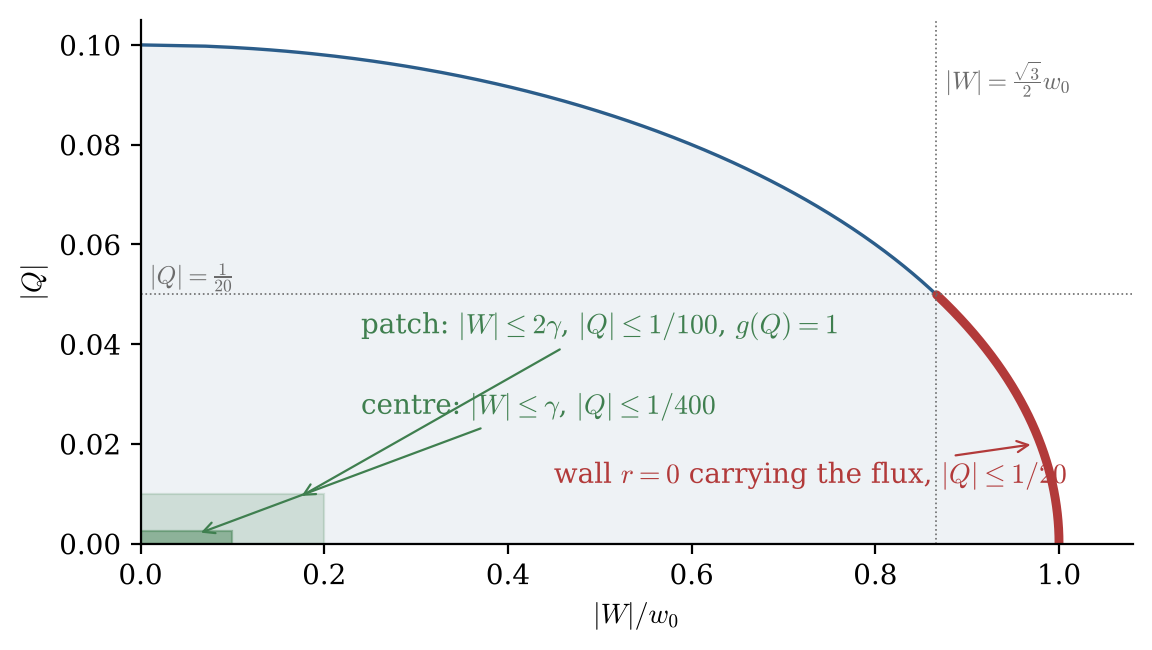
\includegraphics[width=0.92\textwidth]{figures/fig_fibre.png}
\caption{The fixed fibre in the modulus coordinates $(|W|,|Q|)$. The wave flux through the wall
$r=0$ is carried by the heavy arc, where $|Q|\le1/20$ and hence $|W|\ge\sqrt3\,w_0/2$; this
separation from the frequency cap gives the Gaussian decay $e^{-c\,s/h}$. Near the centre, balls
of radius $h$ about points with $|W|\le\gamma$, $|Q|\le1/400$ stay in the patch $|W|\le2\gamma$,
$|Q|\le1/100$, where $g(Q)=1$ and the Gaussian can be inverted at the cost $e^{C\gamma^2s/h}$.}
\label{fig:fibre}
\end{figure}

\subsubsection*{A spatial average for the upper bound}
For a dimensional constant $D\ge1$, fixed below, set
\[
P_*(X)=\bigl(J_{Ds}*|g_T|^2\bigr)(X)^{1/d},\qquad M=2n+4 ,
\]
where convolution is in the real spatial variables and $J_\ell$ is the periodisation of
$c_n\ell^{-n}(1+|X/\ell|^2)^{-M/2}$, of integral one, as in \eqref{eq:regular}. Each derivative of
this kernel costs at most a factor $C\ell^{-1}$ pointwise, $|\nabla^jJ_\ell|\le C\ell^{-j}J_\ell$; hence
$|\nabla^j(J_{Ds}*|g_T|^2)|\le C(Ds)^{-j}J_{Ds}*|g_T|^2$, and taking the $d$th root gives the first
half of
\begin{equation}\label{eq:Pstar}
|\nabla_X^jP_*|\le C(Ds)^{-j}P_*\quad(j=1,2),\qquad\int P_*^{d+1}\,dX\le\|g_T\|_{\pc}^{\pc}.
\end{equation}
The second half is Young's inequality with exponent $q=(d+1)/d$:
$\int P_*^{d+1}=\|J_{Ds}*|g_T|^2\|_q^q\le\||g_T|^2\|_q^q=\|g_T\|_{2q}^{2q}$. The positive kernel gives
$P_*>0$, since $\|g_T\|_2=1$.

We next bound the current $A_{\rm w}$ and its density $\mu$. By Proposition \ref{prop:current},
each real component of $\chi$ is the real or imaginary part of a Fourier multiplier applied to
$g_T$, whose symbol is a bounded smooth factor times
\[
(\kappa/y)^{d/2}e^{-\Psi},\qquad\Psi=\tfrac12\kappa y|W-v|^2,\qquad y=|Y|\asymp s .
\]
Multiply the symbol by a fixed smooth annular cut-off equal to one on the data and supported in
$|v|<w_0/3$. In the variable $\eta=h\xi$ its derivatives through order $M$ are bounded by
$C(hs)^{-d/2}\sigma^m$ for some fixed $m$: on this cut-off $h\kappa$ and $v$ have bounded
derivatives, $h\kappa$ is bounded away from zero, $(\kappa/y)^{d/2}\asymp(hs)^{-d/2}$, and each
derivative of $\Psi=\frac12(h\kappa)(y/h)|W-v|^2$ costs at most $C\sigma$. On the part of the wall
where $g(Q)\ne0$ we have $|W-v|\ge(\sqrt3/2-1/3)w_0$, so the same bound holds with an extra factor
$e^{-c_*\sigma}$, where $c_*>0$ does not depend on $\gamma$.

If $\mathsf B$ bounds the derivatives through order $M$ of a symbol $a(h\xi)$ supported in a fixed
compact set, then applying $(1-\Delta_\eta)^{n+2}$ inside the inverse Fourier transform bounds the
absolute value of its kernel by $C\mathsf Bh^{-n}(1+|X/h|^2)^{-M/2}$. On the torus the kernel of the
multiplier is the periodisation of the Euclidean kernel, so it is majorised by $C\mathsf BJ_h$, also
for a rotated frame. By Cauchy--Schwarz the squared modulus of the output is at most
$C\mathsf B^2J_h*|g_T|^2$. There is one more convolution with $J_h$ in $A_{\rm w}$, and
$J_h*J_h\le CJ_h$: in the Euclidean convolution one of $|Y|$, $|X-Y|$ is at least $|X|/2$, and the
inequality survives periodisation. Moreover $J_h\le(Ds/h)^nJ_{Ds}$, since
$h^{-n}(1+|X/h|^2)^{-M/2}\le(L/h)^nL^{-n}(1+|X/L|^2)^{-M/2}$ for $L=Ds\ge h$. Using
$(hs)^{-d}=s^{-2d}\sigma^d$ and enlarging $m$, we obtain, for the matrix operator norm,
\begin{equation}\label{eq:Aw}
\|A_{\rm w}\|\le Cs^{-2d}\sigma^mP_*^d\quad(r\le0),\qquad
\|A_{\rm w}\|\le Cs^{-2d}\sigma^me^{-c_*\sigma}P_*^d\quad(r=0).
\end{equation}
Only the first bound is needed for $\mu$, whose remaining term is
$h^{50n}\det\Hfib(r)\le Ch^{50n}a^{-2}s^{-2d}$ by Lemma \ref{lem:fibre}. The nearest lattice term of
the kernel gives $\inf_XJ_{Ds}(X)\ge c_Dh^{M-n}$, since the torus has fixed diameter and $h\le s\le3$;
consequently $P_*^d\ge c_Dh^{M-n}\|g_T\|_2^2=c_Dh^{M-n}$, which absorbs $h^{50n}a^{-2}\le h^{50n-2}$.
In particular
\begin{equation}\label{eq:mu}
\mu\le Cs^{-2d}\sigma^mP_*^d\qquad(r\le0).
\end{equation}

\subsubsection*{A comparison function vanishing on the wall}
Put $R=\Hfib(r)$. By Lemma \ref{lem:fibre}, $R\ge cs^{-2}I$ and $\Gfib(r)\Gfib(r)^*\le R$. We claim
\begin{equation}\label{eq:rPstar}
\Hfib(rP_*)\ge(1-C/D)P_*R .
\end{equation}
The product rule \eqref{eq:product} gives $P_*R$, $r\Hfib(P_*)$ and two terms pairing the
gradients of $r$ and $P_*$. For a quaternionic vector $e$, $|e^*\Gfib(r)|\le(e^*Re)^{1/2}$, while
$|e^*\Gfib(P_*)|\le|\nabla P_*||e|\le C(Ds)^{-1}P_*\cdot Cs(e^*Re)^{1/2}$ by \eqref{eq:Pstar} and
$R\ge cs^{-2}I$; this bounds the mixed terms by $CD^{-1}P_*e^*Re$. The term with $\Hfib(P_*)$ is at
most $C(Ds)^{-2}P_*|e|^2\le CD^{-2}P_*e^*Re$ by \eqref{eq:Pstar} and $|r|\le1$.

Since $r<0$, an upper bound for $u/r$ calls for a comparison function below $u$ whose
determinant is at least $\lambda\mu$. Fix $D$ so that the right side of \eqref{eq:rPstar} is at
least $P_*R/2$. For $v_*=C_1\sigma^{m_1}rP_*$ this gives $\Hfib(v_*)\ge\alpha I$ with
$\alpha=cC_1\sigma^{m_1}P_*s^{-2}$. The background $B_{\rm fib}=\lambda\Hfib(|\Phi|^2)$ has rank one
and positive eigenvalue $\beta\asymp\lambda$ by Lemma \ref{lem:fibre}, so by the monotonicity of
$\det$ in Lemma \ref{lem:moore} and \eqref{eq:compress},
\[
\det\bigl(B_{\rm fib}+\Hfib(v_*)\bigr)\ge\det(B_{\rm fib}+\alpha I)=(\beta+\alpha)\alpha^d
\ge c\lambda\bigl(C_1\sigma^{m_1}P_*s^{-2}\bigr)^d\ge\lambda\mu ,
\]
by \eqref{eq:mu}, once $m_1d\ge m$ and $C_1$ is large. The potentials $v_*$ and $u$ have the same
zero boundary values, so the comparison principle in the proof of Theorem \ref{thm:dirichlet}
yields $v_*\le u\le0$. Dividing by $r<0$ and passing to the boundary,
\begin{equation}\label{eq:urho}
0\le u/r\le C_1\sigma^{m_1}P_*\qquad(r\le0).
\end{equation}

By Lemma \ref{lem:comparison}, $\F\le X_0=\int(-u)\mu\,d\zeta$, and $-u=|r|\,(u/r)\le C_1\sigma^{m_1}P_*$.
The volume element in $(P,Z)$ is comparable to $a^2s^{2d}\,dW\,dQ$ on a fixed bounded set, by Lemma
\ref{lem:fibre}, and $P_*$ depends only on $X$. Combining \eqref{eq:Pstar}, \eqref{eq:mu} and
\eqref{eq:urho} therefore gives, after enlarging $m$,
\begin{equation}\label{eq:Fup}
\F(T,\tau)\le Ca^2\sigma^m\|g_T\|_{\pc}^{\pc}.
\end{equation}
For the flux we need the full gradient of $r$. Tangency in Proposition \ref{prop:current} gives
$A_{\rm w}G(|\Phi|^2)=0$, because $G(|\Phi|^2)=2(\partial\Phi)^*\Phi\,\ii$; the remaining part
$w_0^{-2}G(|W|^2)$ has size $O(s^{-1})$ by Lemma \ref{lem:fibre}. Thus
$G(r)^*A_{\rm w}G(r)\le Cs^{-2}\|A_{\rm w}\|$. In the coordinates $(W,Q)$ the function $r$ is fixed
with nonvanishing gradient on the wall, so the coarea formula and Lemma \ref{lem:fibre} give
$\int\delta(r)\,dP\,dZ\le Ca^2s^{2d}$. Inserting the wall bound \eqref{eq:Aw} and \eqref{eq:urho}
into the flux integral of Proposition \ref{prop:balance},
\begin{equation}\label{eq:fluxbound}
\Delta_z\F(T,\tau)\le C(a/s)^2\sigma^me^{-c_*\sigma}\|g_T\|_{\pc}^{\pc}.
\end{equation}

\subsubsection*{Recovering the wave in the interior}
Consider a centre $(X,P,Z)$ with $|W|\le\gamma$ and $|Q|\le1/400$. In the ball of radius $h$
about it in the $3n$ real spatial coordinates, $W=P/Y$ changes by at most $Ch/s\le C/K$ and
$\Phi$ by at most $Ch$, so $Q$ by at most $C/K$. If $K\gamma$ and $K$ are large enough, the ball
lies in $|W|\le2\gamma$, $|Q|\le1/100$, inside the fibre, and the cut-off in $A_{\rm w}$ equals one
throughout it.

The first scalar multiplier $S_0$ of the time component in \eqref{eq:ATT} has symbol
$b_0(\kappa/y)^{d/2}e^{-\Psi}$ with $b_0=(1+\Re(W)\cdot v/2)/\sqrt2$ bounded away from zero, and the
other component is orthogonal, so $|S_0g_T|^2\le A^0_{TT}$. Invert $S_0$ on the frequencies of
$g_T$ by multiplying its reciprocal symbol by a smooth annular cut-off equal to one on the data
and supported in $|v|\le2\gamma$. On its support $|W-v|\le4\gamma$, so $\Psi\le C\gamma^2\sigma$, and
the derivatives of the reciprocal symbol in $\eta=h\xi$ through order $M$ are bounded by
\[
\mathsf B_{\rm inv}=C_\gamma(hs)^{d/2}\sigma^me^{C\gamma^2\sigma};
\]
the derivatives of the cut-off enter only the prefactor $C_\gamma$, and the constant in the
exponential does not depend on $\gamma$. The kernel estimate above yields
$|g_T(X)|^2\le C\mathsf B_{\rm inv}^2(J_h*A^0_{TT})(X)$ for each choice of the imaginary coordinates
in the ball, with $A^0_{TT}$ evaluated at those coordinates. Since $J_h(X-Y)$ and $J_h(X'-Y)$ are
comparable for $|X'-X|\le h$, the density at every point of the ball is at least
\begin{equation}\label{eq:mX}
m_X=c_\gamma(hs)^{-d}\sigma^{-m}e^{-C_2\gamma^2\sigma}|g_T(X)|^2 .
\end{equation}

For the interior lower bound on $-u$ we need a comparison function above $u$. Let $l$ be the
Euclidean distance from the centre. The quadratic $v_b=\eps m_X^{1/d}(l^2-h^2)$ vanishes on the
boundary of the ball and has fibre Hessian $6\eps m_X^{1/d}I$, since there are three real slots
per spatial coordinate. If $m_X>0$, its determinant after adding $B_{\rm fib}$ is
\[
(\beta+6\eps m_X^{1/d})(6\eps m_X^{1/d})^d\le C\bigl((\eps m_X^{1/d})^n+\lambda(\eps m_X^{1/d})^d\bigr)
\le C(\eps^n+\eps^d)\lambda m_X\le\lambda m_X ,
\]
for a fixed small $\eps$, because the density ceiling \eqref{eq:lambda} and \eqref{eq:mX} give
$m_X^{1/d}\le\mu^{1/d}\le\lambda$. Now $u\le0=v_b$ on the boundary of the ball and the
determinant of $B_{\rm fib}+\Hfib(u)$ is $\lambda\mu\ge\lambda m_X$, so the comparison principle on
the ball (Theorem \ref{thm:dirichlet} and its proof) gives $u\le v_b$ there. At the centre the
depth is therefore at least $\eps h^2m_X^{1/d}$, and multiplying by $\mu\ge m_X$ gives
$(-u)\mu\ge\eps h^2m_X^{1+1/d}$, also when $m_X=0$. Here $1+1/d=q$, and $m_X^q$ contains
$|g_T(X)|^{2q}=|g_T(X)|^{\pc}$.

The imaginary volume of the region of centres is comparable to $a^2s^{2d}\gamma^{2d}$. Integrate
the centre inequality over it and over $X$, use the lower bound of Lemma \ref{lem:comparison}, and
note that $h^2s^{2d}(hs)^{-dq}=h^{1-d}s^{d-1}=\sigma^{n-2}$ since $dq=d+1$. Enlarging $m$ and
absorbing $\gamma^{2d}$ into the prefactor,
\begin{equation}\label{eq:Flow}
\F(T,\tau)\ge c_\gamma a^2\sigma^{-m}e^{-C_3\gamma^2\sigma}\|g_T\|_{\pc}^{\pc}.
\end{equation}

Choose $\gamma$ so small that $C_3\gamma^2<c_*/2$, then fix $K$ to meet the ball inclusions and so
that $h<1/(4K)$ lies in the range of \eqref{eq:lambda}. For $f\ne0$ both sides below are positive,
and dividing \eqref{eq:fluxbound} by \eqref{eq:Flow} gives
\[
\frac{\Delta_z\F}{\F}\le C_\gamma s^{-2}\sigma^{2m}e^{-(c_*-C_3\gamma^2)\sigma}.
\]
The exponential absorbs the power of $\sigma$, which proves \eqref{eq:Fsuper}. On the two circles
in the $\tau$-plane the scaled radii $4a/h=4K$ and $2a/h=2K$ are fixed. The upper bound
\eqref{eq:Fup} at $T=0$ on the first circle gives \eqref{eq:Fupper}, and the lower bound
\eqref{eq:Flow} on the second gives \eqref{eq:Flower} for the wave at time $T$.
\end{proof}

\section{Propagation across a thin cylinder}\label{sec:cylinder}

The energy of Proposition \ref{prop:fibre} controls the wave on the circle $|\tau|=2a$ for
$1\le T\le2$, and is controlled by the data on $|\tau|=4a$ at $T=0$. To compare the two sets we
first carry the energy out to $|\tau|=1$, where a fixed neighbourhood connects the two time
intervals, and then carry it back towards the inner wall. Each passage costs one logarithm, as
Figure \ref{fig:cylinder} illustrates. The radial harmonic functions used for comparison are the
probabilities that planar Brownian motion leaves an annulus through one circle or the other
\cite[Theorem 3.18]{MP10}; the maximum principle keeps this comparison in the presence of a
potential.

\begin{figure}[t]
\centering
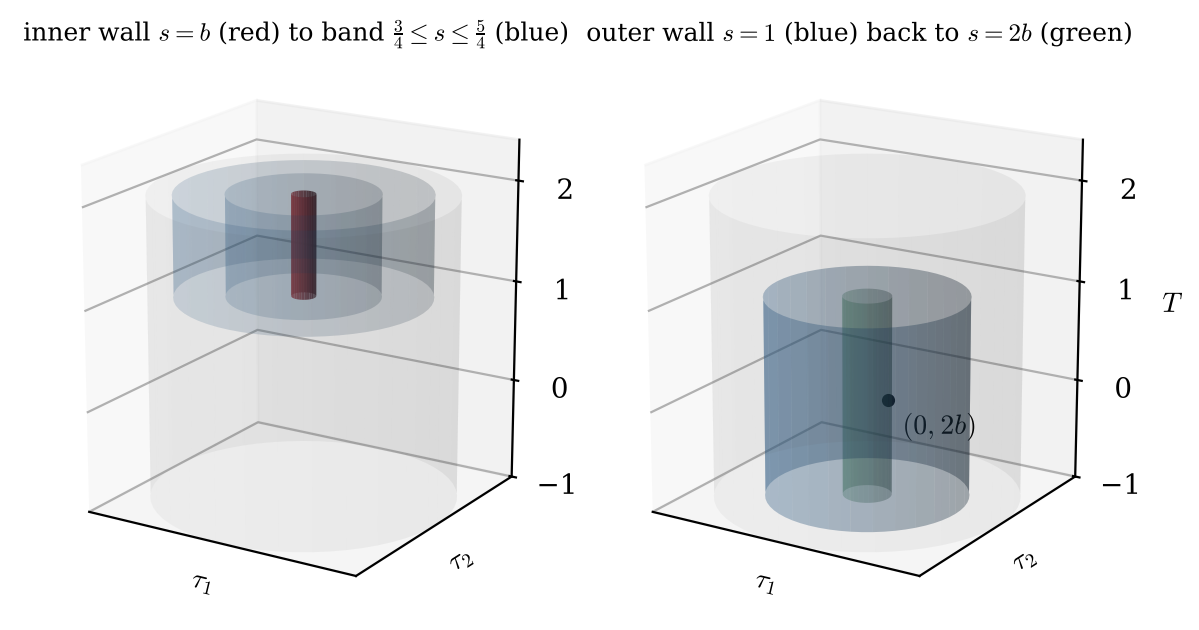
\includegraphics[width=0.95\textwidth]{figures/fig_cylinder.png}
\caption{The two comparisons in the $(T,s)$ half-plane, $s=|\tau|$, drawn schematically. Left: the
mass of the circular mean on the inner wall $s=b$ for $1\le T\le2$ bounds the mass in the band
$3/4\le s\le5/4$ from below, at the cost $1/\log(3/b)$. Right: a mean-value inequality on a fixed
annulus gives a lower bound on the whole outer wall $s=1$, and the comparison solution
$\cos(\pi T/2)u(s)$ carries it back to $s=2b$ at the cost $\log 2/\log(1/b)$. In the wave estimate
$b=2Kh$, the inner wall controls the wave on $1\le T\le2$, and the dot at $(0,2b)$ is controlled by
the initial data.}
\label{fig:cylinder}
\end{figure}

\begin{lemma}[\cite{OAI26}]\label{lem:cylinder}
Let $0<b<1/4$ and $D=\log(3/b)$. Suppose a continuous potential $V:[b,3]\to[0,\infty)$ satisfies
\begin{equation}\label{eq:Vint}
\int_b^3s\log(s/b)\,V(s)\,ds\le M,\qquad\sup_{1/2\le s\le3/2}V(s)\le M .
\end{equation}
Let $E\ge0$ be smooth on $\R_T\times\{\tau\in\R^2:b\le|\tau|\le3\}$ with
$\Delta_{T,\tau}E\le V(|\tau|)E$ in the interior. Its circular mean
\[
H(T,s)=\frac1{2\pi}\int_0^{2\pi}E\bigl(T,s(\cos\theta,\sin\theta)\bigr)\,d\theta
\]
satisfies, for $b\le r\le1$,
\begin{equation}\label{eq:cylinder}
H(0,r)\ge c(M)\,\frac{\log(r/b)}{D^2}\int_1^2H(T,b)\,dT .
\end{equation}
In particular the factor at $r=2b$ is a constant multiple of $D^{-2}$.
\end{lemma}

\begin{proof}
Averaging over rotations preserves the differential inequality, so $H(T,|\tau|)$ is again a
supersolution: $(-\Delta_{T,\tau}+V)H\ge0$. All maximum principles below are the weak maximum
principle for operators $\Delta-c$ with bounded $c\ge0$ \cite[Corollary 3.2]{GT01}.

\emph{Radial comparison functions.} For $S\in\{1,3\}$ and a fixed $\kappa>0$ consider
\[
u''+s^{-1}u'=(V+\kappa^2)u\qquad(b<s<S),
\]
with endpoint values $0,1$ in either order. We claim that $u$ is at least a constant $c(M,\kappa)$
times the function affine in $\log s$ with the same endpoint values. The substitution
$x=\log(s/b)$ gives $u''+s^{-1}u'=s^{-2}u_{xx}$, so the equation becomes $u_{xx}=P(x)u$ on $[0,A]$
with $A=\log(S/b)$ and $P(x)=s^2(V(s)+\kappa^2)\ge0$. Let $\psi$ solve it with $\psi(0)=0$,
$\psi'(0)=1$. Then $\psi''=P\psi\ge0$ while $\psi\ge0$, so $\psi'\ge1$ and $\psi(x)\ge x$. Integrating
twice, $\psi(x)=x+\int_0^x(x-z)P(z)\psi(z)\,dz$, that is,
\[
\frac{\psi(x)}x=1+\int_0^x\frac{z(x-z)}{x}\,P(z)\,\frac{\psi(z)}z\,dz .
\]
Since $z(x-z)/x\le\min(z,A-z)$, Gronwall's inequality gives
$\psi(A)/A\le\exp\bigl(\int_0^A\min(z,A-z)P(z)\,dz\bigr)$. In this integral, $dz=ds/s$ and
$\min(z,A-z)\le\log(s/b)$, so the contribution of $V$ is at most
$\int_b^3s\log(s/b)V(s)\,ds\le M$; with $t=A-z$, $s=Se^{-t}$, the contribution of $\kappa^2$ is at
most $\kappa^2S^2\int_0^\infty te^{-2t}dt$. Hence $\psi(A)\le C(M,\kappa)A$, and the solution
$u=\psi/\psi(A)$ with $u(0)=0$, $u(A)=1$ satisfies $u(x)\ge x/(C(M,\kappa)A)$. The integral bound is
unchanged under $x\mapsto A-x$, which gives the other order of the endpoint values.

\emph{The outward passage.} Put $m(s)=\int_0^3\sin(\pi T/3)H(T,s)\,dT$. The cut-off is positive on
the observed times and its second derivative is a multiple of itself; two integrations by parts
give
\[
\int_0^3\sin(\pi T/3)\,\partial_T^2H(T,s)\,dT=-(\pi/3)^2m(s)+(\pi/3)\bigl(H(0,s)+H(3,s)\bigr).
\]
Since $H\ge0$, multiplying $\partial_T^2H+\partial_s^2H+s^{-1}\partial_sH\le VH$ by $\sin(\pi T/3)$ and
integrating gives $m''+s^{-1}m'\le(V+\pi^2/9)m$. Let $u$ be the radial solution with $S=3$,
$\kappa=\pi/3$, $u(b)=1$ and $u(3)=0$. Then $m-m(b)u$ is a supersolution vanishing at $s=b$ and
nonnegative at $s=3$, so it is nonnegative, and the radial estimate gives
$m(s)\ge c\,m(b)\log(3/s)/D$. In particular
\begin{equation}\label{eq:outward}
\int_0^3\!\!\int_{3/4\le|\tau|\le5/4}H(T,|\tau|)\,d\tau\,dT\ge c\,m(b)/D .
\end{equation}

\emph{A Harnack chain.} On the fixed region $-2<T<4$, $1/2<|\tau|<3/2$ we have $\Delta H\le MH$. The
compact weak Harnack inequality gives $H(T,1)\ge c(M)m(b)/D$ for $|T|\le1$; we give the argument.
Add a real variable $v$. The function $w=H(T,|\tau|)\cos(\sqrt{M+1}\,v)$ satisfies
$\Delta w\le(MH-(M+1)H)\cos(\sqrt{M+1}\,v)\le0$, so it is nonnegative and superharmonic on a fixed slab
$|v|<v_0$. Its mean-value inequality on the four-dimensional ball of radius $2\rho$ about
$(x,0)$, $x=(T,\tau)$, restricted to $|v|<\rho$, where each slice of the ball contains the
three-dimensional ball $B_\rho(x)$ and the cosine is at least $1/2$, gives
\[
H(x)\ge c\rho^{-3}\int_{B_\rho(x)}H
\]
for one small radius $\rho$, throughout a neighbourhood of the compact connected band
$[-1,3]\times\{3/4\le|\tau|\le5/4\}$; here $H(x)=H(T,|\tau|)$. Cover the band by finitely many
balls of radius $\rho/4$. If two of them, $B$ and $B'$, overlap, then $B'\subset B_\rho(x)$ for every
$x\in B$, so $\inf_BH\ge c\rho^{-3}\int_{B'}H$. By \eqref{eq:outward} one ball of the cover carries
at least a fixed fraction of $c\,m(b)/D$, and a finite chain of overlapping balls gives
$H\ge c(M)m(b)/D$ on the whole band.

\emph{The return passage.} Take the radial solution $u$ with $S=1$, $\kappa=\pi/2$, $u(b)=0$ and
$u(1)=1$. On $|T|<1$, $b<|\tau|<1$ the function $w=c(M)m(b)D^{-1}\cos(\pi T/2)u(|\tau|)$ satisfies
$(-\Delta_{T,\tau}+V)w=0$, vanishes on $|T|=1$ and on $|\tau|=b$, and lies below $H$ on $|\tau|=1$ by the
Harnack chain. The maximum principle gives $H\ge w$, and the radial estimate gives
\[
H(0,r)\ge\frac{c(M)m(b)}D\cdot\frac{\log(r/b)}{\log(1/b)}\qquad(b\le r\le1).
\]
Since $\log(1/b)\le D$ and $\sin(\pi T/3)\ge\sqrt3/2$ on $[1,2]$, this proves \eqref{eq:cylinder}.
\end{proof}

\begin{remark}\label{rem:cylinder}
The dependence on $r$ and $b$ in Lemma \ref{lem:cylinder} is sharp for scalar supersolutions,
even when $V=0$. Let $p(s)=\log(3/s)/D$, the radial harmonic function with $p(b)=1$, $p(3)=0$, and
$g(s)=s^2(1+\log(3/s))/(4D)$. A direct computation gives $g''+s^{-1}g'=p$. The radial harmonic
interpolant $L(s)=p(s)g(b)+(1-p(s))g(3)$ satisfies $\Delta_\tau(L-g)=-p\le0$ and $L-g=0$ at $s=b,3$, so
$L\ge g$. Thus $E(T,s)=(1-\cos T)p(s)+L(s)-g(s)$ is bounded and nonnegative, with
$\Delta_{T,\tau}E=(\cos T-1)p\le0$, and its trace at $s=b$ is $1-\cos T$. Since $g$ is increasing,
\[
E(0,r)\le(1-p(r))g(3)=\frac94\,\frac{\log(r/b)}{D^2}.
\]
A fixed positive $r$ would cost one logarithm only; the data control $r=2b$, where a sharper
estimate would need more information about the wave.
\end{remark}

\begin{proposition}[\cite{OAI26}]\label{prop:torus}
On $\T^n=\R^n/(100\Z)^n$ let $f$ have Fourier support in $c_0/h\le|\xi|\le C_0/h$, $0<h\le1$, and in
one cap of the aperture $\gamma$ of Proposition \ref{prop:fibre}. Then
\begin{equation}\label{eq:torus}
\Bigl(\int_1^2\|e^{-iT|D|}f\|_{L^{\pc}(\T^n)}^{\pc}\,dT\Bigr)^{1/\pc}\le C\,[\log(2/h)]^{2/\pc}\,\|f\|_{L^{\pc}(\T^n)} ,
\end{equation}
with $C$ independent of $h$ and of the direction of the cap.
\end{proposition}

\begin{proof}
Both sides are homogeneous, so for $f\ne0$ we may normalise $\|f\|_{L^2(\T^n)}=1$. Fix the
constant $K$ of Proposition \ref{prop:fibre}, put $a=Kh$ and $b=2a$, and first take $h$ so small
that $b<1/4$. Apply Lemma \ref{lem:cylinder} to the energy $E=\F\ge0$ of that proposition, with
$V(s)=Cs^{-2}e^{-cs/h}$; the energy is defined for $a<|\tau|<4$, and \eqref{eq:Fsuper} holds on
$b\le|\tau|\le3$. The first bound in \eqref{eq:Vint} follows from the substitution $s=bt$,
\[
\int_b^3s\log(s/b)V(s)\,ds\le C\int_1^\infty\frac{\log t}{t}\,e^{-2cKt}\,dt ,
\]
and $V\le4C$ on $1/2\le s\le3/2$. The bounds \eqref{eq:Fupper} and \eqref{eq:Flower} are uniform on
their circles, so the circular mean satisfies
\[
H(0,2b)\le Ca^2\|f\|_{\pc}^{\pc},\qquad H(T,b)\ge ca^2\|e^{-iT|D|}f\|_{\pc}^{\pc}.
\]
Take $r=2b$ in \eqref{eq:cylinder}, insert both bounds, cancel $a^2$ and take $\pc$-th roots; since
$D=\log(3/(2Kh))\lesssim\log(2/h)$, this gives \eqref{eq:torus}. For the remaining $h$, bounded
below, the frequencies lie in a fixed finite set, and \eqref{eq:torus} holds because
$\|e^{-iT|D|}f\|_\infty\le\sum|\hat f|\le C\|f\|_1\le C\|f\|_{\pc}$ on such functions.
\end{proof}

\section{Euclidean space, local smoothing and Bochner--Riesz means}\label{sec:euclid}

The aperture in Proposition \ref{prop:torus} is fixed, so a finite partition of the sphere gives
the critical estimate on a whole annulus with the same power of the logarithm. We remove the
spatial period, interpolate, sum the dyadic annuli, and then deduce the Bochner--Riesz
conjecture. Throughout, $I=[1,2]$.

\subsection{Removing the period}\label{ssec:period}
\begin{proof}[Proof of Theorem \ref{thm:annular}]
Write $h=N^{-1}$ and $P_h=\varphi(hD)$, with $\varphi$ supported in a fixed compact annulus
$c_0\le|\eta|\le C_0$. Choose a smooth finite partition $\varphi=\sum_\nu\varphi_\nu$ subordinate to
caps of aperture $\gamma$ about finitely many directions. On the torus $\T^n=\R^n/(100\Z)^n$ the
multiplier $\varphi_\nu(hD)$ has as kernel the periodisation of the Euclidean kernel
$h^{-n}\check\varphi_\nu(\cdot/h)$, and periodisation does not increase the $L^1$ norm, so
$\|\varphi_\nu(hD)f\|_{L^{\pc}(\T^n)}\le C\|f\|_{L^{\pc}(\T^n)}$. Applying Proposition \ref{prop:torus}
to each $\varphi_\nu(hD)f$, in the frame of its cap, and summing over $\nu$ gives
\begin{equation}\label{eq:torusall}
\|U(T)P_hf\|_{L^{\pc}(I\times\T^n)}\lesssim[\log(2/h)]^{2/\pc}\|f\|_{L^{\pc}(\T^n)},\qquad0<h\le1/2 .
\end{equation}
The Euclidean kernel of $U(T)P_h$ is
\[
K_h(T,X)=(2\pi h)^{-n}\int e^{i(X\cdot\eta-T|\eta|)/h}\varphi(\eta)\,d\eta .
\]
For $T\in I$ and $|X|\ge3$ the gradient of the phase before division by $h$, $X-T\eta/|\eta|$, has
length at least $|X|-2\ge|X|/3$. Integrating by parts along this gradient gains a factor $h/|X|$
each time, since the amplitude is supported away from $\eta=0$ and all phase derivatives of order
at least two are bounded there. With $M+n$ integrations,
\begin{equation}\label{eq:Kdecay}
|K_h(T,X)|\le C_Mh^M(1+|X|)^{-M}\qquad(T\in I,\ |X|\ge3).
\end{equation}

Tile $\R^n$ by unit cubes $Q$ and let $10Q$ be the concentric cube of side ten. If $X\in Q$ and
$Y\notin10Q$ then $|X-Y|\ge9/2$, so on $Q$ the contribution of $f1_{(10Q)^c}$ is bounded pointwise by
$C_Mh^M\bigl((1+|\cdot|)^{-M}*|f|\bigr)(X)$. This single function bounds the far contributions on every
cube, and for $M>n$ Young's inequality bounds its $L^{\pc}(I\times\R^n)$ norm by $O(h^M)\|f\|_{\pc}$.

Translate the centre of $Q$ to the origin and periodise $f_Q=f1_{10Q}$ on the torus of side $100$;
its torus norm is $\|f\|_{L^{\pc}(10Q)}$. The periodic wave kernel is the periodisation of $K_h$. On
$Q$ its nonzero translates see only arguments $X-Y+100k$ with $Y\in10Q$ and $k\in\Z^n\setminus\{0\}$;
since $|X_j-Y_j|\le11/2$, each coordinate satisfies $|X_j-Y_j+100k_j|\ge\frac{189}2|k_j|$, so these
arguments have length at least $\frac{189}2|k|$. Summing \eqref{eq:Kdecay} over $k$ bounds the
difference between the periodic and Euclidean outputs on $Q$ by $C_Mh^M\|f_Q\|_1\le C_Mh^M\|f\|_{L^{\pc}(10Q)}$.
Hence \eqref{eq:torusall} gives
\[
\|U(T)P_hf_Q\|_{L^{\pc}(I\times Q)}\lesssim[\log(2/h)]^{2/\pc}\|f\|_{L^{\pc}(10Q)} .
\]
Take $\pc$-th powers and sum over $Q$. The cubes $10Q$ have bounded overlap, so together with the
far contributions this proves Theorem \ref{thm:annular}, since $\log(2/h)\asymp\log(2+N)$ for
$N\ge2$.
\end{proof}

\subsection{Interpolation and summation}\label{ssec:interp}
By Plancherel the norm of $U(T)P_h$ from $L^2(\R^n)$ to $L^2(I\times\R^n)$ is at most
$\|\varphi\|_\infty$, since $|I|=1$. From $L^\infty$ to $L^\infty$ its norm is $O(h^{-d/2})$. To see
this, partition the annulus into $O(h^{-d/2})$ caps of aperture $c\sqrt h$ with bounded overlap. In
coordinates $\eta=(\sqrt h\,z,\rho)$, $z\in\R^d$, about the axis of a cap, its cut-off is supported in
a fixed compact set with $\rho$ bounded below and has uniformly bounded derivatives; such cut-offs
are obtained by dividing rescaled angular bumps by their sum, and the overlapping centres have
bounded offsets in these coordinates. The linear phase $T\rho/h$ corresponds to a translation in
the axis direction, and what remains of the phase is
\[
\frac Th\Bigl(\sqrt{\rho^2+h|z|^2}-\rho\Bigr)=\frac{T|z|^2}{\sqrt{\rho^2+h|z|^2}+\rho},
\]
which has uniformly bounded derivatives on the support. In these coordinates the kernel of a
cap equals $(2\pi)^{-n}h^{-n+d/2}\check b(X'/\sqrt h,X_n/h)$, up to that translation, for a smooth
$b$ with bounded support and derivatives, so its $L^1$ norm is
$(2\pi)^{-n}h^{-n+d/2+d/2+1}\|\check b\|_1=O(1)$. Summing over the caps gives the bound.

Set $\beta(p)=\min\{d(1-2/p),2/p\}$. Riesz--Thorin interpolation \cite[Ch.~1]{Gra14} of Theorem
\ref{thm:annular} with these two bounds gives
\begin{equation}\label{eq:interp}
\|U(T)P_hf\|_{L^p(I\times\R^n)}\lesssim_ph^{-s_+(p)}[\log(2/h)]^{\beta(p)}\|f\|_{L^p(\R^n)},\qquad2\le p\le\infty .
\end{equation}
Indeed, for $2\le p\le\pc$ write $\frac12-\frac1p=\theta(\frac12-\frac1{\pc})=\frac\theta{2n}$; the power of the
logarithm is $2\theta/\pc=n(1-\frac2p)\frac{d}{n}=d(1-\frac2p)$. For $\pc\le p\le\infty$ write $\frac1p=\frac{1-\theta}{\pc}$;
the power of the logarithm is $2(1-\theta)/\pc=2/p$ and that of $h^{-1}$ is
$\frac d2(1-\frac{\pc}p)=\frac d2-\frac np$. The two expressions for $\beta$ agree at $p=\pc$, and the minimum
selects the correct one on each side.

\begin{proof}[Proof of Theorem \ref{thm:ls}]
Let $\varphi$ define a smooth dyadic partition $\chi_0(\xi)+\sum_{j\ge1}\varphi(2^{-j}\xi)=1$, and set
$g=J^{s_+(p)+\eps}f$. With $h=2^{-j}$, \eqref{eq:interp} bounds the $j$th piece by
$C2^{-j\eps}(1+j)^{\beta(p)}\|g\|_p$: a smooth enlargement of $\varphi(2^{-j}\cdot)$ times
$2^{j(s_+(p)+\eps)}J^{-s_+(p)-\eps}$ is a multiplier whose kernel is uniformly integrable. These
bounds are summable in $j$. On the low frequencies the symbol $\chi_0(\xi)e^{-iT|\xi|}J(\xi)^{-s_+(p)-\eps}$
satisfies the Mihlin conditions uniformly in $T\in I$, so it is bounded on $L^p$ for $1<p<\infty$
\cite[Ch.~6]{Gra14}. At $p=2$ Plancherel gives the estimate without loss.
\end{proof}

A finer summation gives the estimate at the exact exponent $s_+(p)$ with logarithmic factors
\cite[Corollary 7.1]{OAI26}; it is not needed here.

\subsection{Bochner--Riesz means}\label{ssec:br}
The Bochner--Riesz mean $B^\alpha_r$ has multiplier $(1-|\xi|^2/r^2)^\alpha_+$; write
$B^\alpha_*f=\sup_{r>0}|B^\alpha_rf|$. A smooth cut-off to a shell of relative width $\delta$ is an
average of waves over times of order $\delta^{-1}$, which is how local smoothing controls these
means. Sogge observed the implication for a single radius \cite[(4.5)--(4.6)]{Sog91}, and Beltran,
Hickman and Sogge give the fixed-radius and maximal reductions \cite[Propositions 39 and 40]{BHS21}.

\begin{theorem}[Bochner--Riesz means \cite{OAI26}]\label{thm:BR}
Let $n\ge2$, $1\le p\le\infty$, and $\delta(p)=\max\{0,n|1/p-1/2|-1/2\}$. If $\alpha>\delta(p)$, then
\begin{equation}\label{eq:BRall}
\sup_{r>0}\|B^\alpha_rf\|_{L^p(\R^n)}\le C_{n,p,\alpha}\|f\|_{L^p(\R^n)} ,
\end{equation}
and $B^\alpha_rf\to f$ in $L^p$ as $r\to\infty$ when $p<\infty$. If $2\le p<\infty$ and
$\alpha>s_+(p)$, then $\|B^\alpha_*f\|_p\le C_{n,p,\alpha}\|f\|_p$.
\end{theorem}

For $1\le p<2n/(n+1)$ we have $\delta(p)=\lambda(p)$ of \eqref{eq:critical}. We first rescale Theorem
\ref{thm:ls} to a unit frequency annulus and a long time interval: for $2\le p<\infty$,
$\sigma>s_+(p)$ and $\hat g$ supported in a fixed annulus $c\le|\xi|\le C$,
\begin{equation}\label{eq:longtime}
\|U(t)g\|_{L^p(\R^n\times\{R\le|t|\le2R\})}\lesssim R^{1/p+\sigma}\|g\|_p,\qquad R\ge1 .
\end{equation}
Indeed $g(R\,\cdot)$ has frequencies of order $R$ and $U(t)[g(R\,\cdot)](x)=(U(Rt)g)(Rx)$. Changing
variables in space and time contributes $R^{(n+1)/p}$, Theorem \ref{thm:ls} with the Sobolev
multiplier on that annulus contributes $O(R^\sigma)$, and the input norm contributes $R^{-n/p}$.
Complex conjugation gives the negative times, since $\overline{U(t)g}=U(-t)\bar g$. For $|t|\le1$ the
unit annular wave multiplier has a uniformly integrable kernel.

\begin{lemma}[Maximal estimate for a thin shell \cite{OAI26}]\label{lem:shell}
For $0<\delta\le1/8$ and $\psi\in C_c^\infty((1/2,2))$ let
$A_{\delta,r}f=\psi\bigl((1-|D|/r)/\delta\bigr)f$. For $2\le p<\infty$ and $\sigma>s_+(p)$,
\[
\Bigl\|\sup_{r>0}|A_{\delta,r}f|\Bigr\|_p\lesssim\delta^{-\sigma}\|f\|_p ,
\]
uniformly for $\psi$ in bounded subsets of $C_c^\infty((1/2,2))$.
\end{lemma}

\begin{proof}
For $1\le r\le2$ the shell lies in $1/2<|\xi|<2$. Choose a smooth annular symbol $\chi$ equal to one
there, let $Q_k=\chi(2^{-k}D)$ and $g=Q_0f$. Writing $\psi$ by Fourier inversion and substituting
$\tau=\delta rt$,
\[
A_{\delta,r}f(x)=\frac{\delta r}{2\pi}\int_\R e^{itr}\,\hat\psi(\delta rt)\,U(t)g(x)\,dt .
\]
Taking the supremum over $r\in[1,2]$ bounds this by $C_M\delta\int(1+\delta|t|)^{-M}|U(t)g(x)|\,dt$. On a
dyadic interval $R\le|t|\le2R$, H\"older's inequality in time and \eqref{eq:longtime} bound the $L^p_x$
norm of this contribution by $C_M\delta(1+\delta R)^{-M}R^{1-1/p}R^{1/p+\sigma}\|g\|_p$. For $M>1+\sigma$ the
sum over dyadic $R\ge1$ is $O(\delta^{-\sigma}\|g\|_p)$, as one sees by splitting at $R=\delta^{-1}$; the
interval $|t|\le1$ contributes $O(\delta\|g\|_p)$.

For $r=2^ks$ with $1\le s\le2$ set $g_k(y)=(Q_kf)(2^{-k}y)$. Then $A_{\delta,r}f(2^{-k}y)=A_{\delta,s}g_k(y)$,
and the factor $2^{-kn/p}$ in the output norm cancels $2^{kn/p}$ in $\|g_k\|_p$. So the $L^p$ norm of the
supremum over this octave is at most $C\delta^{-\sigma}\|Q_kf\|_p$. The supremum over all octaves is at
most their pointwise $\ell^p$ norm, and since $p\ge2$, Littlewood--Paley theory gives
$(\sum_k\|Q_kf\|_p^p)^{1/p}\le\|(\sum_k|Q_kf|^2)^{1/2}\|_p\lesssim\|f\|_p$.
\end{proof}

\begin{proof}[Proof of Theorem \ref{thm:BR}]
Take $2\le p<\infty$ and $s_+(p)<\sigma<\alpha$. Choose $\eta\in C_c^\infty((1/2,2))$ with
$\sum_{j\in\Z}\eta(2^jv)=1$ for $v>0$, and apply this partition to $v=1-\rho$ on $0\le\rho<1$. For
$\delta=2^{-j}\le1/8$ the corresponding term is
\[
\eta\bigl(2^j(1-\rho)\bigr)(1-\rho^2)^\alpha=\delta^\alpha\psi_\delta\bigl((1-\rho)/\delta\bigr),\qquad
\psi_\delta(u)=\eta(u)u^\alpha(2-\delta u)^\alpha ,
\]
because $1-\rho^2=(1-\rho)(1+\rho)$ and $1+\rho=2-\delta u$. These profiles have uniformly bounded
smooth seminorms. The remaining terms, $0\le j\le2$, add up to a smooth radial multiplier of compact
support which vanishes near $\rho=1$ and equals $(1-\rho^2)^\alpha$ near $\rho=0$; the supremum of its
dilations is bounded by a constant times the Hardy--Littlewood maximal function, since its kernel
has a radially decreasing integrable majorant. Lemma \ref{lem:shell} bounds the other terms of
$B^\alpha_*$ by $C\sum_{j\ge3}2^{-j(\alpha-\sigma)}\|f\|_p$. This proves the maximal estimate.

For $2\le p<\infty$, $\delta(p)=s_+(p)$, so the maximal estimate implies \eqref{eq:BRall}. Each $B^\alpha_r$
is self-adjoint and $\delta(p)=\delta(p')$, so duality gives \eqref{eq:BRall} for $1<p<2$. At $p=1$ and
$p=\infty$ the hypothesis is $\alpha>(n-1)/2$; the unit-radius kernel is a constant multiple of
$|x|^{-n/2-\alpha}J_{n/2+\alpha}(|x|)$ \cite[Ch.~IX]{Ste93}, bounded at the origin and
$O(|x|^{-(n+1)/2-\alpha})$ at infinity, hence integrable, and its dilates $r^nK(rx)$ have a common $L^1$
norm. Finally, for Schwartz functions with compactly supported Fourier transform the multipliers
converge to one in all derivatives on the support as $r\to\infty$, so the means converge in the
Schwartz topology; density and \eqref{eq:BRall} give convergence in $L^p$ for $p<\infty$.
\end{proof}

\part*{Part II. Removal of the $\varepsilon$-loss}
\section{Removal of the \texorpdfstring{$\varepsilon$}{epsilon}-loss}\label{sec:vbr}

Theorem \ref{thm:BR} bounds the Bochner--Riesz means of every order $\lambda>\lambda(p)$, with constants
that grow as $\lambda\downarrow\lambda(p)$. To reach the critical index we need a multi-scale form of
these bounds without the loss, the inequalities $\VBR(p,r)$ below. That they follow from the
non-endpoint bounds is Tao's $\varepsilon$-removal \cite{Tao98}; the off-diagonal form, with $r>p$, is
due to Beltran, Roos and Seeger \cite{BRS23}. This section reproduces their argument for the round
sphere $\rho(\xi)=|\xi|$, which is the only case needed here. We follow \cite{BRS23} step by step and
write out the computations it leaves to the reader. The letter $\ell$ indexes the dyadic layers that
\cite{BRS23} index by $n$, since $n$ is the dimension here.

\subsection{Statement}\label{ssec:vbrstatement}
A dyadic lattice $\D$ is a family of half-open cubes as in \cite[\S2]{LN19}: the subfamily $\D_j$ of
cubes of side $2^j$ partitions $\R^n$ for every $j\in\Z$, and the cubes of $\D_{j-1}$ inside a cube of
$\D_j$ are its $2^n$ halves. Then $\D_0=\{a+z+[0,1)^n:z\in\Z^n\}$ for some $a\in\R^n$, and for $j\ge0$
every cube of $\D_j$ is a union of cubes of $\D_0$. For $M\ge1$ let $\Y_M$ be the set of $C^M$
functions $\chi$ on $\R$ with support in a compact subset of $(\frac12,2)$ and
$\sum_{\nu=0}^M\|\chi^{(\nu)}\|_\infty\le1$. Throughout this section we fix an integer $N\ge3n+1$, put
$M_0=N+n+1$, and write $\Y=\Y_{M_0}$.

\begin{definition}\label{def:vbr}
Let $1\le p\le r<\infty$. The statement $\VBR(p,r)$ is: there are $M$ and $C$ such that for every
dyadic lattice $\D$, all $\chi_j\in\Y_M$ ($j\ge1$) and all families $\{f_Q\}_{Q\in\D}$ of functions
$f_Q\in L^p(\R^n)$ with $\supp f_Q\subset Q$,
\begin{equation}\label{eq:vbr}
\Bigl\|\sum_{j\ge1}2^{j\frac{n+1}2}\chi_j\bigl(2^j(1-|D|)\bigr)\sum_{Q\in\D_j}f_Q\Bigr\|_{L^r(\R^n)}
\le C\Bigl(\sum_{Q\in\D}|Q|\,\|f_Q\|_{L^p(\R^n)}^r\Bigr)^{1/r}.
\end{equation}
\end{definition}

This is \cite[Definition 2.2]{BRS25} and \cite[Definition 1.1]{BRS23} for the unit ball. It suffices to
prove \eqref{eq:vbr} for families with finitely many nonzero members: for a general family with finite
right-hand side, the partial sums of the left-hand side over increasing finite subfamilies then form a
Cauchy sequence in $L^r$, since the difference of two partial sums is itself such a sum, and
\eqref{eq:vbr} passes to the limit. Applied to a single cube, \eqref{eq:vbr} gives
$\|\chi(2^j(1-|D|))\|_{L^p\to L^r}\lesssim 2^{j\lambda(r)}$, with $\lambda(r)=n(\frac1r-\frac12)-\frac12$ as in
\eqref{eq:critical}; summing a decomposition of $(1-|\xi|)^{\lambda}_+$ into such bumps then bounds the
Riesz means of every order $\lambda>\lambda(r)$, so $\VBR(p,r)$ is a multi-scale strengthening of these
bounds.

Write $p_{\rm ST}=\frac{2(n+1)}{n+3}$ for the Stein--Tomas exponent. For $p_{\rm ST}<p_\circ<\frac{2n}{n+1}$
and $p_{\rm ST}\le p\le p_\circ$ define $r_*(p)=r_*(p,p_\circ)$ by
\begin{equation}\label{eq:rstar}
\frac1{r_*(p)}=\frac{\frac1{p_\circ}\bigl(\frac1{p_{\rm ST}}-\frac1p\bigr)+\frac12\bigl(\frac1p-\frac1{p_\circ}\bigr)}
{\frac1{p_{\rm ST}}-\frac1{p_\circ}} .
\end{equation}
Thus $1/r_*$ is the affine function of $1/p$ equal to $\frac12$ at $p=p_{\rm ST}$ and to $\frac1{p_\circ}$
at $p=p_\circ$: the pair $(\frac1p,\frac1{r_*(p)})$ runs along the segment from $(\frac1{p_{\rm ST}},\frac12)$
to $(\frac1{p_\circ},\frac1{p_\circ})$. Since both endpoints satisfy $\frac1r\le\frac1p$ and $\frac1r\ge\frac12$,
\begin{equation}\label{eq:rstarrange}
p\le r_*(p)\le 2\qquad(p_{\rm ST}\le p\le p_\circ).
\end{equation}
As $p_\circ\to\frac{2n}{n+1}$ the denominator of \eqref{eq:rstar} tends to
$\frac{n+3}{2(n+1)}-\frac{n+1}{2n}=\frac{n-1}{2n(n+1)}$ and the numerator to
$\frac{n+1}{2n}\bigl(\frac{n+3}{2(n+1)}-\frac1p\bigr)+\frac12\bigl(\frac1p-\frac{n+1}{2n}\bigr)=\frac1{2n}\bigl(1-\frac1p\bigr)$,
so
\begin{equation}\label{eq:rstarlimit}
\lim_{p_\circ\to\frac{2n}{n+1}}\frac1{r_*(p,p_\circ)}=\frac{n+1}{n-1}\Bigl(1-\frac1p\Bigr),\qquad
\lim_{p_\circ\to\frac{2n}{n+1}}r_*(p,p_\circ)=\frac{n-1}{n+1}\,p' .
\end{equation}
This is the line $r=\frac{n-1}{n+1}p'$ of the Knapp examples, which bounds the range of $\VBR(p,r)$
\cite[\S1]{BRS23}.

The multiplier $(1-|\xi|)^\lambda_+$ is not smooth at the origin, which plays no role in the
problem. We therefore work with a localised form. Fix $\tilde w\in C^\infty_c((\frac18,2))$ with $\tilde w=1$ on
$[\frac14,\frac32]$ and set
\begin{equation}\label{eq:Rlambda}
R^\lambda=\tilde w(|D|)\,(1-|D|)^\lambda_+\qquad(\lambda>-1).
\end{equation}

\begin{theorem}[{\cite[Theorem 1.2]{BRS23}}]\label{thm:vbr}
Let $n\ge2$ and $p_{\rm ST}<p_\circ<\frac{2n}{n+1}$, and suppose that $R^\lambda$ is bounded on
$L^{p_\circ}(\R^n)$ for every $\lambda>\lambda(p_\circ)$. Then $\VBR(p,r)$ holds for
$p_{\rm ST}\le p<p_\circ$ and $p\le r<r_*(p,p_\circ)$, with $M=M_0$.
\end{theorem}

In \cite{BRS23} the hypothesis is an $L^{p_\circ}\to L^{r_\circ}$ bound with $r_\circ\ge p_\circ$; we
need only $r_\circ=p_\circ$, since the limit \eqref{eq:rstarlimit} already reaches the Knapp line.

\begin{lemma}\label{lem:riesz}
\begin{enumerate}[label=\textup{(\roman*)}]
\item If $1\le p\le\infty$ and $(1-|D|^2)^\lambda_+$ is bounded on $L^p$, then so is $R^\lambda$. In
particular, $R^\lambda$ is bounded on $L^p$ for $1\le p<\frac{2n}{n+1}$ and $\lambda>\lambda(p)$.
\item For $\lambda>-\frac12$, $R^\lambda$ maps $L^{p_{\rm ST}}(\R^n)$ to $L^2(\R^n)$.
\end{enumerate}
\end{lemma}

\begin{proof}
(i) On the support of $\tilde w(|\xi|)$ we have $(1-|\xi|)^\lambda_+=(1-|\xi|^2)^\lambda_+(1+|\xi|)^{-\lambda}$, so
$R^\lambda=a(D)\,(1-|D|^2)^\lambda_+$ with $a(\xi)=\tilde w(|\xi|)(1+|\xi|)^{-\lambda}$. The function $a$ is smooth,
since $\tilde w(|\xi|)$ vanishes near the origin, and has compact support; so its kernel is a Schwartz
function and $a(D)$ is bounded on every $L^p$. The second statement is Theorem \ref{thm:BR} with $r=1$,
since $\delta(p)=\lambda(p)$ for $p<\frac{2n}{n+1}$.

(ii) By Plancherel's theorem and polar coordinates,
\[
\|R^\lambda f\|_2^2=(2\pi)^{-n}\int_0^1\tilde w(t)^2(1-t)^{2\lambda}t^{n-1}\int_{S^{n-1}}|\hat f(t\omega)|^2\,d\sigma(\omega)\,dt .
\]
For $\frac18\le t\le1$, $\hat f(t\,\cdot)$ is the Fourier transform of $t^{-n}f(\cdot/t)$, whose
$L^{p_{\rm ST}}$ norm is $t^{-n/p_{\rm ST}'}\|f\|_{p_{\rm ST}}\le 8^n\|f\|_{p_{\rm ST}}$. The Stein--Tomas
restriction theorem \cite[Ch.~IX, \S2.1]{Ste93} bounds the inner integral by $C\|f\|_{p_{\rm ST}}^2$, and
$\int_0^1(1-t)^{2\lambda}\,dt<\infty$ for $\lambda>-\frac12$.
\end{proof}

\begin{corollary}\label{cor:vbr}
Let $n\ge2$. For every $p_\circ\in(p_{\rm ST},\frac{2n}{n+1})$, $\VBR(p,r)$ holds for $p_{\rm ST}\le p<p_\circ$
and $p\le r<r_*(p,p_\circ)$. Consequently $\VBR(p,r)$ holds whenever $p_{\rm ST}\le p<\frac{2n}{n+1}$ and
$p\le r<\frac{n-1}{n+1}p'$.
\end{corollary}

\begin{proof}
By Lemma \ref{lem:riesz}(i) the hypothesis of Theorem \ref{thm:vbr} holds for every
$p_\circ<\frac{2n}{n+1}$, which gives the first statement. For the second, given $p<\frac{2n}{n+1}$ and
$r<\frac{n-1}{n+1}p'$, the limit \eqref{eq:rstarlimit} provides $p_\circ\in(p,\frac{2n}{n+1})$ with
$r<r_*(p,p_\circ)$.
\end{proof}

The rest of this section proves Theorem \ref{thm:vbr}; its hypothesis is assumed from now on, and
implicit constants may depend on $n$, $p_\circ$, $N$ and the exponents at hand, but not on the
lattice, the cubes, the functions or the bumps $\chi_j$.

\subsection{Single-scale estimates}\label{ssec:singlescale}
For $j\ge1$ and $\chi\in\Y$ let
\begin{equation}\label{eq:mj}
m_j(\xi)=h_j(|\xi|),\qquad h_j(\varrho)=\chi\bigl(2^j(1-\varrho)\bigr),
\end{equation}
so that $m_j$ is supported in $1-2^{1-j}<|\xi|<1-2^{-j-1}$. The two coarsest scales need no
analysis.

\begin{lemma}\label{lem:twoscales}
Let $j\in\{1,2\}$, $1\le p\le r<\infty$, and $\chi\in\Y_M$ with $M\ge n+1$. Then the kernel $K_j$ of
$m_j(D)$ satisfies $|K_j(x)|\le C(1+|x|)^{-n-1}$, and
\[
\Bigl\|m_j(D)\sum_{Q\in\D_j}f_Q\Bigr\|_r\le C\Bigl(\sum_{Q\in\D_j}\|f_Q\|_p^r\Bigr)^{1/r}
\qquad(\supp f_Q\subset Q).
\]
\end{lemma}

\begin{proof}
Write $g(t)=\chi(2^j(1-t))$. For $j=2$, $g$ vanishes on $[0,\frac12]$, so $m_2$ is smooth and
$|\partial^\alpha m_2|\le C$ for $|\alpha|\le M$. For $j=1$, extend $\chi$ by zero; it is then $C^M$
on $\R$ and vanishes on $[2,\infty)$, so $g^{(i)}(0)=0$ for $i\le M$ and Taylor's formula gives
$|g^{(i)}(t)|\le2^Mt^{M-i}$ for $0\le t\le1$ and $i\le M$. For $\xi\ne0$ and $1\le|\alpha|\le M$ the
chain rule gives
\begin{equation}\label{eq:faa}
\partial^\alpha\bigl[g(|\xi|)\bigr]=\sum_{i=1}^{|\alpha|}g^{(i)}(|\xi|)\,P_{i,\alpha}(\xi),
\end{equation}
where $P_{i,\alpha}$ is a sum of products of $i$ derivatives of $|\xi|$ of total order $|\alpha|$; it is
smooth on $\xi\ne0$, homogeneous of degree $i-|\alpha|$, and independent of $g$. Hence
$|\partial^\alpha m_1(\xi)|\le C|\xi|^{M-|\alpha|}\le C$ on $0<|\xi|<1$. So $m_1$ is $C^{M-1}$ on $\R^n$,
with derivatives of order $M-1$ that are Lipschitz, and its distributional derivatives of order $M$
are bounded. In both cases $|x^\alpha K_j(x)|\le(2\pi)^{-n}\|\partial^\alpha m_j\|_{L^1}\le C$ for
$|\alpha|\le M$, which gives the kernel bound since $M\ge n+1$.

For the second assertion,
\[
|K_j*f_Q(x)|\le C(1+\dist(x,Q))^{-n-1}\|f_Q\|_1\le C'(1+\dist(x,Q))^{-n-1}\|f_Q\|_p ,
\]
because $|Q|\le4^n$. For $x$ in a cube $Q'\in\D_j$ this gives
$\bigl|\sum_QK_j*f_Q(x)\bigr|\le C\sum_Q(1+|c_Q-c_{Q'}|)^{-n-1}\|f_Q\|_p$, with $c_Q$ the centre of $Q$.
The right-hand side is the convolution, on the lattice of centres, of $(\|f_Q\|_p)_Q$ with a summable
sequence, so its $\ell^r$ norm over $Q'$ is at most $C(\sum_Q\|f_Q\|_p^r)^{1/r}$. Integrating over each
$Q'$, of measure at most $4^n$, gives the claim.
\end{proof}

From now on $j\ge3$, so that $m_j$ is supported in $\frac34<|\xi|<1$. By \eqref{eq:faa}, for
$1\le|\alpha|\le M_0$,
\begin{equation}\label{eq:dmj}
\partial^\alpha m_j(\xi)=\sum_{k=1}^{|\alpha|}(-2^j)^k\,\chi^{(k)}\bigl(2^j(1-|\xi|)\bigr)\,P_{k,\alpha}(\xi),
\qquad |\partial^\alpha m_j(\xi)|\le C\,2^{j|\alpha|} ,
\end{equation}
since $|P_{k,\alpha}|\le C$ on $\frac34\le|\xi|\le1$.

\subsubsection*{Subordination}
For $c>0$ and a continuous function $g$ on $\R$ whose support is bounded above, with enough decay at
$-\infty$, let
\[
I^cg(\varrho)=\frac1{\Gamma(c)}\int_\varrho^\infty(s-\varrho)^{c-1}g(s)\,ds .
\]
For compactly supported $g$, Fubini's theorem and the Beta integral give $I^aI^cg=I^{a+c}g$; and
$I^1(-g')=g$ for $g\in C^1_c$, so $I^k((-\tfrac{d}{d\varrho})^kg)=g$ for $g\in C^k_c$.

\begin{lemma}[{\cite[(2.3) and Lemma 2.1]{BRS23}}]\label{lem:subord}
Let $\lambda>-1$, let $k=\lfloor\lambda\rfloor+2$, so that $b=k-\lambda-1\in(0,1]$, and let $h\in C^k_c(\R)$.
Put $H=I^b\bigl((-\tfrac{d}{d\varrho})^kh\bigr)$. Then
\begin{equation}\label{eq:subord}
h(\varrho)=\frac1{\Gamma(\lambda+1)}\int_\varrho^\infty(s-\varrho)^{\lambda}H(s)\,ds\qquad(\varrho\in\R).
\end{equation}
If $h=h_j$ with $j\ge3$ and $\|\chi\|_{C^k}\le1$, then $H(s)=0$ for $s\ge1-2^{-j-1}$,
\begin{equation}\label{eq:Hbound}
|H(s)|\le C\,\frac{2^{j(\lambda+1)}}{\bigl(1+2^j(1-s)\bigr)^{\lambda+2}}\quad(s<1),\qquad
\int_{5/8}^1|H(s)|\,ds\le C\,2^{j\lambda}.
\end{equation}
\end{lemma}

\begin{proof}
The function $(-\frac d{d\varrho})^kh$ has compact support, so
$I^{\lambda+1}H=I^{\lambda+1}I^b(-\tfrac{d}{d\varrho})^kh=I^k(-\tfrac{d}{d\varrho})^kh=h$, which is
\eqref{eq:subord}. Now let $h=h_j$, supported in $[1-2^{1-j},1-2^{-j-1}]$, with
$|h_j^{(k)}|\le2^{jk}$. If $b=1$ then $H=(-1)^{k-1}h_j^{(k-1)}$, which is supported in the same interval
and bounded by $2^{j(k-1)}=2^{j(\lambda+1)}$; this gives \eqref{eq:Hbound}. Let $0<b<1$. Clearly $H(s)=0$ for
$s\ge1-2^{-j-1}$. If $1-2^{2-j}\le s<1$, then
\[
|H(s)|\le\frac{2^{jk}}{\Gamma(b)}\int_s^1(u-s)^{b-1}\,du\le\frac{2^{jk}(1-s)^b}{\Gamma(b+1)}\le C\,2^{j(k-b)}=C\,2^{j(\lambda+1)} .
\]
If $s<1-2^{2-j}$, then $u-s\ge\frac12(1-s)$ on the support of $h_j$, and $h_j$ vanishes near $u=s$, so
$k$ integrations by parts give
\[
|H(s)|=\frac1{\Gamma(b)}\Bigl|\int(b-1)\cdots(b-k)\,(u-s)^{b-1-k}h_j(u)\,du\Bigr|
\le C\,2^{-j}\Bigl(\frac{1-s}2\Bigr)^{-\lambda-2}=C\,\frac{2^{j(\lambda+1)}}{(2^j(1-s))^{\lambda+2}} ,
\]
since $b-1-k=-\lambda-2$. This proves the pointwise bound. Integrating it over $[\frac58,1]$, the part
$1-s\le2^{2-j}$ contributes $C2^{j(\lambda+1)}2^{2-j}$ and the rest
$C2^{-j}\int_{2^{2-j}}^{\infty}t^{-\lambda-2}\,dt\le C2^{j\lambda}$, because $\lambda+1>0$.
\end{proof}

\subsubsection*{Spatial localisation}
Fix a radial $\phi_0\in C^\infty_c(\R^n)$ with $\phi_0(x)=1$ for $|x|\le\frac12$ and $\phi_0(x)=0$ for
$|x|\ge1$, and set
\begin{equation}\label{eq:phijl}
\phi_{j,0}(x)=\phi_0(2^{-j}x),\qquad \phi_{j,\ell}(x)=\phi_0(2^{-j-\ell}x)-\phi_0(2^{-j-\ell+1}x)\quad(\ell\ge1),
\end{equation}
so that $\sum_{\ell\ge0}\phi_{j,\ell}=1$, $\phi_{j,\ell}$ is supported in $|x|<2^{j+\ell}$, and for $\ell\ge1$ it
vanishes on $|x|\le2^{j+\ell-2}$. Let
\begin{equation}\label{eq:mjl}
m_{j,\ell}=(2\pi)^{-n}\,m_j*\widehat{\phi_{j,\ell}} .
\end{equation}
Then $m_{j,\ell}(D)$ has kernel $K_j\phi_{j,\ell}$, where $K_j$ is the kernel of $m_j(D)$; so this kernel
is supported in $|x|<2^{j+\ell}$, $m_j=\sum_\ell m_{j,\ell}$, and $m_{j,\ell}$ is radial. Since
$\phi_{j,\ell}=\phi_{0,1}(2^{1-j-\ell}\,\cdot)$ for $\ell\ge1$,
\begin{equation}\label{eq:phihat}
|\widehat{\phi_{j,\ell}}(\eta)|\le C_K\,2^{(j+\ell)n}(1+2^{j+\ell}|\eta|)^{-K},\qquad
\int|\eta|^N|\widehat{\phi_{j,\ell}}(\eta)|\,d\eta\le C\,2^{-(j+\ell)N},
\end{equation}
for every $K$, and $\int\eta^\beta\widehat{\phi_{j,\ell}}(\eta)\,d\eta=(2\pi)^n(i\partial)^\beta\phi_{j,\ell}(0)=0$
for every multi-index $\beta$ when $\ell\ge1$. Taylor's formula for $m_j(\xi-\eta)$ about $\xi$, to
order $N$, therefore gives for $\ell\ge1$
\begin{equation}\label{eq:taylor}
m_{j,\ell}(\xi)=(2\pi)^{-n}\sum_{|\alpha|=N}\frac N{\alpha!}\int\!\!\int_0^1(1-s)^{N-1}(-\eta)^\alpha\,
\partial^\alpha m_j(\xi-s\eta)\,ds\;\widehat{\phi_{j,\ell}}(\eta)\,d\eta .
\end{equation}

\begin{lemma}[{\cite[(2.13)]{BRS23}}]\label{lem:mjlpoint}
For $j\ge3$, $\ell\ge0$ and every $N_1$,
\[
|m_{j,\ell}(\xi)|\le C_{N_1}\,2^{-\ell N}\bigl(1+2^j\bigl||\xi|-1\bigr|\bigr)^{-N_1}.
\]
\end{lemma}

\begin{proof}
Let $t=||\xi|-1|$. Let $\ell\ge1$. By \eqref{eq:dmj} and \eqref{eq:phihat}, \eqref{eq:taylor} gives
$|m_{j,\ell}(\xi)|\le C2^{jN}2^{-(j+\ell)N}=C2^{-\ell N}$. If $t\ge2^{2-j}$, the integrand of \eqref{eq:taylor}
vanishes unless $||\xi-s\eta|-1|<2^{1-j}$, which forces $|\eta|\ge s|\eta|\ge t-2^{1-j}\ge t/2$; by
\eqref{eq:phihat} with $K=N+n+N_1$,
\[
|m_{j,\ell}(\xi)|\le C2^{jN}\int_{|\eta|\ge t/2}|\eta|^N2^{(j+\ell)n}(1+2^{j+\ell}|\eta|)^{-K}\,d\eta
\le C2^{-\ell N}(1+2^{j+\ell}t)^{-N_1}.
\]
For $\ell=0$, $|m_{j,0}(\xi)|\le C\int_{||\xi-\eta|-1|<2^{1-j}}2^{jn}(1+2^j|\eta|)^{-K}d\eta$, which is bounded,
and is at most $C(1+2^jt)^{-N_1}$ when $t\ge2^{2-j}$ by the same argument.
\end{proof}

\begin{lemma}[{\cite[Lemma 2.2]{BRS23}}]\label{lem:single}
Let $1\le p\le r<\infty$ and $-1<\lambda<n-1$, and suppose that $R^\lambda$ maps $L^p$ to $L^r$. Let
$j\ge3$ and $\ell\ge0$.
\begin{enumerate}[label=\textup{(\roman*)}]
\item If $\chi\in C^{n+1}$ is supported in $(\frac12,2)$ with $\|\chi\|_{C^{n+1}}\le1$, then
$\|m_j(D)\|_{L^p\to L^r}\le C2^{j\lambda}$.
\item If $\chi\in\Y$, then $\|m_{j,\ell}(D)\|_{L^p\to L^r}\le C2^{-\ell N}2^{j\lambda}$.
\item If $\chi\in\Y$ and $p\le q\le r$, then
$\|m_{j,\ell}(D)\|_{L^p\to L^q}\le C2^{-\ell(N-n)}2^{j(\lambda+n(\frac1q-\frac1r))}$ and
$\|m_j(D)\|_{L^p\to L^q}\le C2^{j(\lambda+n(\frac1q-\frac1r))}$.
\end{enumerate}
\end{lemma}

\begin{proof}
(i) Fix a radial $\theta_1\in C^\infty_c$ supported in $\frac58<|\xi|<\frac54$ and equal to one on
$\frac34\le|\xi|\le1$. By \eqref{eq:subord} with $\varrho=|\xi|$, and since $H_j$ vanishes on $[1,\infty)$,
\[
m_j(\xi)=\theta_1(\xi)m_j(\xi)=\frac1{\Gamma(\lambda+1)}\int_0^1s^\lambda H_j(s)\,\theta_1(\xi)\Bigl(1-\frac{|\xi|}s\Bigr)^\lambda_+ds .
\]
The integrand vanishes for $s<\frac58$. For $\frac58\le s<1$, on the support of $\theta_1(\xi)(1-|\xi|/s)_+$
we have $\frac58<|\xi|/s<1$, where $\tilde w(|\xi|/s)=1$; so the multiplier there is $\theta_1(\xi)$ times the
dilate by $s$ of the symbol of $R^\lambda$, whose $L^p\to L^r$ norm is $s^{n(\frac1p-\frac1r)}\|R^\lambda\|_{L^p\to L^r}$.
By Minkowski's inequality and \eqref{eq:Hbound} (note $k\le n+1$),
$\|m_j(D)\|_{L^p\to L^r}\le C\int_{5/8}^1|H_j(s)|\,ds\le C2^{j\lambda}$.

(ii) For $\ell=0$, \eqref{eq:mjl} writes $m_{j,0}$ as an average of the translates $m_j(\cdot-\eta)$
against the weight $(2\pi)^{-n}|\widehat{\phi_{j,0}}|$, of bounded $L^1$ norm; translating a multiplier
conjugates it by a modulation, which does not change its norm. For $\ell\ge1$ use \eqref{eq:taylor}
and \eqref{eq:dmj}. Let $\theta\in C^\infty_c(\{\frac12<|\xi|<\frac32\})$ be equal to one on
$\frac34\le|\xi|\le1$. Then $\partial^\alpha m_j=\sum_k(-2^j)^k\,(\theta P_{k,\alpha})(\xi)\,\chi^{(k)}(2^j(1-|\xi|))$, where
$\theta P_{k,\alpha}$ is a fixed smooth compactly supported multiplier, bounded on $L^r$, and
$\chi^{(k)}\in C^{M_0-k}$ with $M_0-k\ge n+1$. By (i), $\|\partial^\alpha m_j(D-s\eta)\|_{L^p\to L^r}\le C2^{jN}2^{j\lambda}$ for
$|\alpha|=N$, and \eqref{eq:phihat} gives $\|m_{j,\ell}(D)\|_{L^p\to L^r}\le C2^{jN+j\lambda}2^{-(j+\ell)N}$.

(iii) Let $\mathcal G$ be the grid of cubes of side $2^{j+\ell}$. For a cube $Q\in\mathcal G$ the
function $m_{j,\ell}(D)[f1_Q]$ is supported in the concentric cube $3Q$, and these cubes overlap at most
$3^n$ times. By H\"older's inequality on $3Q$ and (ii),
\begin{align*}
\|m_{j,\ell}(D)f\|_q&\le C\Bigl(\sum_{Q\in\mathcal G}\bigl(|3Q|^{\frac1q-\frac1r}\|m_{j,\ell}(D)[f1_Q]\|_r\bigr)^q\Bigr)^{1/q}\\
&\le C2^{(j+\ell)n(\frac1q-\frac1r)}2^{-\ell N}2^{j\lambda}\Bigl(\sum_Q\|f1_Q\|_p^q\Bigr)^{1/q},
\end{align*}
and $(\sum_Q\|f1_Q\|_p^q)^{1/q}\le\|f\|_p$ since $q\ge p$. Summing over $\ell$ gives the bound for $m_j$,
because $N>n$.
\end{proof}

\begin{corollary}[{\cite[Corollary 2.3]{BRS23}}]\label{cor:single}
Let $p_{\rm ST}\le p_1<p_\circ$ and $p_1\le r\le r_*(p_1)$. For every $\varepsilon>0$, $j\ge3$, $\ell\ge0$ and
$\chi\in\Y$,
\[
\|m_{j,\ell}(D)\|_{L^{p_1}\to L^r}\le C_\varepsilon2^{-\ell(N-n)}2^{j(\lambda(r)+\varepsilon)},\qquad
\|m_j(D)\|_{L^{p_1}\to L^r}\le C_\varepsilon2^{j(\lambda(r)+\varepsilon)} ,
\]
and $R^\lambda$ maps $L^{p_1}$ to $L^r$ for every $\lambda>\lambda(r)$.
\end{corollary}

\begin{proof}
By Lemma \ref{lem:single}(ii), the hypothesis of Theorem \ref{thm:vbr} with $\lambda=\lambda(p_\circ)+\varepsilon$
(which is less than $n-1$), and Lemma \ref{lem:riesz}(ii) with $\lambda=-\frac12+\varepsilon$,
\[
\|m_{j,\ell}(D)\|_{L^{p_\circ}\to L^{p_\circ}}\le C_\varepsilon2^{-\ell N}2^{j(\lambda(p_\circ)+\varepsilon)},\qquad
\|m_{j,\ell}(D)\|_{L^{p_{\rm ST}}\to L^2}\le C_\varepsilon2^{-\ell N}2^{j(\lambda(2)+\varepsilon)},
\]
where $\lambda(2)=-\frac12$. Write $\frac1{p_1}=\frac\vartheta{p_\circ}+\frac{1-\vartheta}{p_{\rm ST}}$ with
$\vartheta\in(0,1]$; then $\frac1{r_*(p_1)}=\frac\vartheta{p_\circ}+\frac{1-\vartheta}2$ by \eqref{eq:rstar}, and since
$\lambda(r)$ is an affine function of $\frac1r$, $\vartheta\lambda(p_\circ)+(1-\vartheta)\lambda(2)=\lambda(r_*(p_1))$. The
Riesz--Thorin theorem gives the first bound for $r=r_*(p_1)$, with $2^{-\ell N}$. For
$p_1\le r<r_*(p_1)$ apply the H\"older argument of Lemma \ref{lem:single}(iii) to this bound, noting that
$\lambda(r_*(p_1))+n(\frac1r-\frac1{r_*(p_1)})=\lambda(r)$; summing in $\ell$ bounds $m_j(D)$.

For the last statement choose $\chi_0\in C^\infty_c((\frac12,2))$ with $\sum_{j\in\Z}\chi_0(2^js)=1$ for $s>0$.
For $j\ge3$, $(1-\varrho)^\lambda\chi_0(2^j(1-\varrho))=2^{-j\lambda}\tilde\chi(2^j(1-\varrho))$ with
$\tilde\chi(s)=s^\lambda\chi_0(s)$, a fixed multiple of an element of $\Y$, and these terms live in
$\frac34<\varrho<1$, where $\tilde w=1$. By the first part their multiplier norms are at most
$C2^{-j(\lambda-\lambda(r)-\varepsilon)}$, which is summable for $\varepsilon<\lambda-\lambda(r)$. The remaining part of the
symbol of $R^\lambda$, $\tilde w(|\xi|)(1-|\xi|)^\lambda_+\bigl(1-\sum_{j\ge3}\chi_0(2^j(1-|\xi|))\bigr)$, is smooth
and supported in $\frac18<|\xi|<\frac78$, so its kernel is a Schwartz function and it maps $L^{p_1}$ to
$L^r$ by Young's inequality.
\end{proof}

\begin{lemma}[{\cite[Lemma 2.5]{BRS23}}]\label{lem:kappa}
For $j\ge3$ and $\ell\ge0$ let $\kappa_{j,\ell}=\F^{-1}\bigl[|m_{j,\ell}|^2\bigr]$. Then
\[
\sup_{x\in\R^n}(1+|x|)^{\frac{n-1}2}|\kappa_{j,\ell}(x)|\le C\,2^{-2\ell N}2^{-j}.
\]
\end{lemma}

\begin{proof}
Since $m_{j,\ell}$ is radial, $|m_{j,\ell}(\xi)|^2=G(|\xi|)$, and in polar coordinates
\[
\kappa_{j,\ell}(x)=(2\pi)^{-n}\int_0^\infty G(t)\,t^{n-1}\,\hat\sigma(tx)\,dt,\qquad
\hat\sigma(y)=\int_{S^{n-1}}e^{i\ip y\omega}\,d\sigma(\omega).
\]
The Fourier transform of the surface measure satisfies $|\hat\sigma(y)|\le C(1+|y|)^{-\frac{n-1}2}$
\cite[Ch.~VIII, \S3.1]{Ste93}; it is a constant multiple of $|y|^{-\frac{n-2}2}J_{\frac{n-2}2}(|y|)$. Hence
\[
|\kappa_{j,\ell}(x)|\le C\min\Bigl\{\int_0^\infty|G(t)|t^{n-1}\,dt,\;|x|^{-\frac{n-1}2}\int_0^\infty|G(t)|t^{\frac{n-1}2}\,dt\Bigr\}.
\]
By Lemma \ref{lem:mjlpoint} with $N_1=n$, $|G(t)|\le C2^{-2\ell N}(1+2^j|t-1|)^{-2n}$, and both integrals are
at most $C2^{-2\ell N}2^{-j}$.
\end{proof}

Lemma \ref{lem:kappa} replaces the stationary phase argument of \cite{BRS23}, which is needed there for
general convex domains; for the sphere the radial symmetry reduces it to the decay of $\hat\sigma$.

\subsection{Square functions over separated cubes}\label{ssec:separated}
The gain over the trivial $L^2$ bound comes from cubes that are far apart, as in Tao's work
\cite{Tao98}. Fix $\psi\in C^\infty_c(\R^n)$ with $\psi\ge0$, $\psi\ne0$ and support in
$|\xi|\le\frac1{4\sqrt n}$, let $\check\psi=\F^{-1}\psi$, and put
\[
\eta=\frac{|\check\psi|^2}{c_0},\qquad c_0=\bigl(\cos(\tfrac12)\,\check\psi(0)\bigr)^2 .
\]
Then $\eta\ge0$ is a Schwartz function, $\hat\eta=c_0^{-1}(2\pi)^{-n}\psi*\psi(-\,\cdot)$ is supported in
$|\xi|\le\frac1{2\sqrt n}$, and $\eta(x)\ge1$ for $|x|_\infty\le2$: for such $x$ and $\xi\in\supp\psi$ we have
$|\ip x\xi|\le2\sqrt n\cdot\frac1{4\sqrt n}=\frac12$, so
$\Re\check\psi(x)=(2\pi)^{-n}\int\psi(\xi)\cos\ip x\xi\,d\xi\ge\cos(\frac12)\check\psi(0)>0$. For a cube $B$ of
side $R\ge1$ and centre $x_B$ let
\begin{equation}\label{eq:etaB}
\eta_B(x)=\eta\Bigl(\frac{x-x_B}R\Bigr),\qquad \widehat{\eta_B}(\xi)=R^ne^{-i\ip{x_B}\xi}\hat\eta(R\xi),
\end{equation}
so that $\widehat{\eta_B}$ is supported in $|\xi|\le\frac1{2R}$, $\eta_B\ge1$ on the concentric cube of side
$4R$, and $\|\eta_B\|_1=R^n\|\eta\|_1$.

\begin{definition}\label{def:separated}
Let $R\ge1$ and $S\ge3R$. A family $\cB$ of cubes of side $R$ is \emph{$S$-separated} if
$|x_B-x_{B'}|\ge S$ for all $B\ne B'$ in $\cB$.
\end{definition}

With $\phi_0$ as in \eqref{eq:phijl} let
\begin{equation}\label{eq:etaBl}
\eta_{B,0}(x)=\phi_0\Bigl(\frac{x-x_B}R\Bigr)\eta_B(x),\qquad
\eta_{B,\ell}(x)=\Bigl[\phi_0\Bigl(\frac{x-x_B}{2^\ell R}\Bigr)-\phi_0\Bigl(\frac{x-x_B}{2^{\ell-1}R}\Bigr)\Bigr]\eta_B(x)
\quad(\ell\ge1).
\end{equation}
Then $\eta_B=\sum_{\ell\ge0}\eta_{B,\ell}$, $\eta_{B,\ell}$ is supported in the ball $|x-x_B|\le2^\ell R$, and
since $\eta_{B,\ell}$ vanishes on $|x-x_B|\le2^{\ell-2}R$ for $\ell\ge1$ and $\eta$ is a Schwartz function,
\begin{equation}\label{eq:etaBlsup}
\|\eta_{B,\ell}\|_\infty\le C_K2^{-\ell K}\qquad\text{for every }K .
\end{equation}

We need one elementary bound on the measure of thin shells. Here and below $B(c,\rho)$ is the ball
of centre $c$ and radius $\rho$.

\begin{lemma}\label{lem:shellmeasure}
Let $K\ge n+1$ and $j\ge0$.
\begin{enumerate}[label=\textup{(\roman*)}]
\item For $c\in\R^n$ and $\rho>0$,
$\displaystyle\int_{B(c,\rho)}\bigl(1+2^j\bigl||w|-1\bigr|\bigr)^{-K}dw\le C\,2^{-j}\min\{\rho,1\}^{n-1}$.
\item For $0<\rho\le1$ and $\xi\in\R^n$,
$\displaystyle\int\rho^{-n}\Bigl(1+\frac{|v|}\rho\Bigr)^{-K}\bigl(1+2^j\bigl||\xi-v|-1\bigr|\bigr)^{-K}dv
\le C\min\{1,2^{-j}\rho^{-1}\}$.
\end{enumerate}
\end{lemma}

\begin{proof}
(i) In polar coordinates the integral over all of $\R^n$ is
$|S^{n-1}|\int_0^\infty(1+2^j|s-1|)^{-K}s^{n-1}ds\le C2^{-j}$, which settles $\rho\ge1$. Let $\rho<1$ and
$V(t)=|\{w\in B(c,\rho):||w|-1|\le t\}|$. If $t\ge\frac12$ then $V(t)\le C\rho^n\le2Ct\rho^{n-1}$. If
$t<\frac12$, then $V(t)=\int_{1-t}^{1+t}\sigma_s(B(c,\rho))\,ds$, where $\sigma_s$ is the surface measure of
the sphere of radius $s\in[\frac12,\frac32]$; a ball of radius $\rho$ meets such a sphere in a set of
diameter at most $2\rho$, of measure at most $C\rho^{n-1}$, so $V(t)\le Ct\rho^{n-1}$. Splitting the
integral according to $||w|-1|\le2^{-j}$ and $2^{i-1-j}<||w|-1|\le2^{i-j}$, $i\ge1$, it is at most
$\sum_{i\ge0}2^{-(i-1)K}V(2^{i-j})\le C\rho^{n-1}2^{-j}\sum_i2^{i-(i-1)K}$.

(ii) The integral is at most $\int\rho^{-n}(1+|v|/\rho)^{-K}dv=C$. Apply (i), with centre $\xi$ and $w=\xi-v$,
on $|v|\le\rho$ and on the shells $2^{i-1}\rho<|v|\le2^i\rho$, $i\ge1$: the contribution of the $i$-th
piece is at most $C\rho^{-n}2^{-(i-1)K}2^{-j}(2^i\rho)^{n-1}$, and the sum over $i$ is
$C2^{-j}\rho^{-1}$.
\end{proof}

\begin{lemma}[{\cite[Lemma 3.3]{BRS23}}]\label{lem:TT}
Let $j\ge3$, $\ell_1,\ell_2\ge0$, $R\ge1$, $S\ge3R$, and let $\cB$ be a finite $S$-separated family of cubes
of side $R$. For every $N_2>0$,
\[
\Bigl\|m_{j,\ell_1}(D)\sum_{B\in\cB}\eta_{B,\ell_2}f_B\Bigr\|_2\le C\,2^{-\ell_1N}2^{-\ell_2N_2}(2^{-j}R)^{1/2}
\Bigl(1+S^{-\frac{n-1}2}R^{n-1}\#\cB\Bigr)^{1/2}\Bigl(\sum_{B\in\cB}\|f_B\|_2^2\Bigr)^{1/2}
\]
for all $f_B\in L^2(\R^n)$, where $C$ depends on $N_2$.
\end{lemma}

\begin{proof}
Let $m=m_{j,\ell_1}$ and $\kappa=\kappa_{j,\ell_1}=\F^{-1}[|m|^2]$. First assume the stronger separation
\begin{equation}\label{eq:strongsep}
|x_B-x_{B'}|\ge S+2^{\ell_2+1}R\qquad(B\ne B'\text{ in }\cB).
\end{equation}
Since $\eta_{B,\ell_2}$ is real, the square of the left-hand side is
$\sum_{B,B'}\ip{T_{B,B'}f_B}{f_{B'}}$, where $T_{B,B'}f=\eta_{B',\ell_2}\,|m|^2(D)[\eta_{B,\ell_2}f]$ has kernel
$\eta_{B',\ell_2}(x)\kappa(x-y)\eta_{B,\ell_2}(y)$.

\emph{Diagonal terms.} If $x,y\in\supp\eta_{B,\ell_2}$, then $|x-y|\le2^{\ell_2+1}R$, so
$\phi_0((x-y)/(2^{\ell_2+2}R))=1$ and the kernel of $T_{B,B}$ is
$\eta_{B,\ell_2}(x)\,\F^{-1}[a](x-y)\,\eta_{B,\ell_2}(y)$ with
\[
a(\xi)=(2\pi)^{-n}\int|m(\xi-v)|^2(2^{\ell_2+2}R)^n\hat\phi_0(2^{\ell_2+2}Rv)\,dv .
\]
Thus $\|T_{B,B}\|_{L^2\to L^2}\le\|\eta_{B,\ell_2}\|_\infty^2\|a\|_\infty$. By Lemma \ref{lem:mjlpoint} with
$N_1=n+1$, $|m(\xi-v)|^2\le C2^{-2\ell_1N}(1+2^j||\xi-v|-1|)^{-n-1}$, and $|\hat\phi_0(u)|\le C(1+|u|)^{-n-1}$; so
Lemma \ref{lem:shellmeasure}(ii) with $\rho=(2^{\ell_2+2}R)^{-1}$ gives
$\|a\|_\infty\le C2^{-2\ell_1N}\min\{1,2^{\ell_2+2-j}R\}$. With \eqref{eq:etaBlsup},
\[
\sum_{B}|\ip{T_{B,B}f_B}{f_B}|\le C_K2^{-2\ell_1N}2^{-\ell_2(2K-1)}2^{-j}R\sum_B\|f_B\|_2^2 .
\]

\emph{Off-diagonal terms.} If $B\ne B'$, $x\in\supp\eta_{B',\ell_2}$ and $y\in\supp\eta_{B,\ell_2}$, then
$|x-y|\ge|x_B-x_{B'}|-2^{\ell_2+1}R\ge S$ by \eqref{eq:strongsep}, so Lemma \ref{lem:kappa} and
\eqref{eq:etaBlsup} bound the kernel of $T_{B,B'}$ by
$C_K2^{-2\ell_1N}2^{-j}S^{-\frac{n-1}2}2^{-2\ell_2K}$ times the indicator of a product of two balls of radius
$2^{\ell_2}R$. By Schur's test
$\|T_{B,B'}\|\le C_K2^{-2\ell_1N}2^{-j}S^{-\frac{n-1}2}2^{-\ell_2(2K-n)}R^n$, and by the Cauchy--Schwarz
inequality
\begin{align*}
\sum_{B\ne B'}|\ip{T_{B,B'}f_B}{f_{B'}}|&\le\max_{B\ne B'}\|T_{B,B'}\|\Bigl(\sum_B\|f_B\|_2\Bigr)^2\\
&\le C_K2^{-2\ell_1N}2^{-\ell_2(2K-n)}2^{-j}R\,S^{-\frac{n-1}2}R^{n-1}\#\cB\sum_B\|f_B\|_2^2 .
\end{align*}
Adding the two bounds proves the lemma under \eqref{eq:strongsep}, with $2^{-\ell_2(2K-n)}$ in place of
$2^{-2\ell_2N_2}$.

\emph{Colouring.} In general, let $T'=S+2^{\ell_2+1}R$ and partition $\R^n$ into the half-open cubes of a grid
of side $a=S/\sqrt n$. Two points of one such cube are at distance less than $S$, so each cube contains at
most one centre $x_B$. Colour the cubes of the grid by their integer coordinates modulo
$k_0=\lceil T'/a\rceil+1$. Points of two different cubes of the same colour are at distance more than
$(k_0-1)a\ge T'$, so each colour class of $\cB$ satisfies \eqref{eq:strongsep}; and since $R\le S/3$, the number
of colours is $k_0^n\le(\sqrt n(1+2^{\ell_2})+2)^n\le C2^{\ell_2n}$. Applying the bound already proved to each
class, with $\#\cB$ in place of the size of the class, and using the Cauchy--Schwarz inequality over the
classes, we lose a factor $C2^{\ell_2n/2}$. Choosing $K$ with $2K-n\ge2N_2+n$ proves the lemma.
\end{proof}

\begin{proposition}[{\cite[Proposition 3.2]{BRS23}}]\label{prop:sep}
Let $j\ge3$ and $1\le R\le2^j$. For each $Q\in\D_j$ let $S_Q\ge3R$ and let $\cB_Q$ be a finite $S_Q$-separated
family of cubes of side $R$ meeting $Q$. Put $\Lambda=\sup_Q(1+S_Q^{-\frac{n-1}2}R^{n-1}\#\cB_Q)^{1/2}$. Then
\begin{align}
\Bigl\|m_j(D)\sum_{Q\in\D_j}\sum_{B\in\cB_Q}\eta_Bf_{Q,B}\Bigr\|_2
&\le C(2^{-j}R)^{1/2}\Lambda\Bigl(\sum_Q\sum_B\|f_{Q,B}\|_2^2\Bigr)^{1/2},\label{eq:sepL2}\\
\Bigl\|m_j(D)\sum_{Q\in\D_j}\sum_{B\in\cB_Q}\eta_Bf_{Q,B}\Bigr\|_1
&\le C2^{j\frac{n-1}2}R^{1/2}\Lambda\sum_Q\Bigl(\sum_B\|f_{Q,B}\|_2^2\Bigr)^{1/2}\label{eq:sepL1}
\end{align}
for all families of functions $f_{Q,B}\in L^2(\R^n)$ with finitely many nonzero members.
\end{proposition}

\begin{proof}
Write the operator as $\sum_{\ell_1,\ell_2\ge0}m_{j,\ell_1}(D)\sum_Q\sum_B\eta_{B,\ell_2}f_{Q,B}$ and fix
$\ell_1,\ell_2$. Let $g_Q=m_{j,\ell_1}(D)\sum_{B\in\cB_Q}\eta_{B,\ell_2}f_{Q,B}$. Every $B\in\cB_Q$ meets $Q$ and has
side $R\le2^j$, so its centre lies within $\frac{\sqrt n}2R\le\sqrt n2^{j+\ell_1}$ of $Q$; the kernel of
$m_{j,\ell_1}(D)$ is supported in $|x|<2^{j+\ell_1}$. Hence $g_Q$ is supported in the set of points at
distance at most $U_0=2^{\ell_2}R+(1+\sqrt n)2^{j+\ell_1}$ from $Q$, and $U_0\le3\sqrt nU$ with
$U=\max\{2^{j+\ell_1},2^{\ell_2}R\}$.

The cubes of $\D_j$ are $Q_k=a_j+2^j(k+[0,1)^n)$, $k\in\Z^n$, for some $a_j\in\R^n$. Colour $Q_k$ by $k$
modulo $k_0=\lceil 2U_02^{-j}\rceil+2$. Two different cubes of the same colour are at distance at least
$(k_0-1)2^j>2U_0$, so within a colour class the $g_Q$ have disjoint supports and
$\|\sum_Qg_Q\|_2^2=\sum_Q\|g_Q\|_2^2$. Lemma \ref{lem:TT} bounds each $\|g_Q\|_2$. The number of classes is
$k_0^n\le C(2^{-j}U)^n\le C2^{(\ell_1+\ell_2)n}$, because $R\le2^j$; the Cauchy--Schwarz inequality over the
classes gives
\begin{equation}\label{eq:sepfixed}
\Bigl\|\sum_Qg_Q\Bigr\|_2\le C2^{-\ell_1(N-\frac n2)}2^{-\ell_2(N_2-\frac n2)}(2^{-j}R)^{1/2}\Lambda
\Bigl(\sum_Q\sum_B\|f_{Q,B}\|_2^2\Bigr)^{1/2} .
\end{equation}
With $N_2=2n+1$ the sum over $\ell_1,\ell_2$ converges, since $N\ge3n+1$; this proves \eqref{eq:sepL2}.

For \eqref{eq:sepL1}, partition $\R^n$ into the cubes $\square$ of a grid of side $s_0=\sqrt n2^j+2U_0\le CU$.
The set of points within $U_0$ of a cube $Q\in\D_j$ has diameter at most $s_0$ and therefore meets at
most $2^n$ cubes $\square$. Let $\cQ(\square)$ be the set of $Q$ for which it meets $\square$. By the
Cauchy--Schwarz inequality on $\square$ and \eqref{eq:sepfixed} applied to the subfamily $\cQ(\square)$,
\begin{align*}
\Bigl\|\sum_Qg_Q\Bigr\|_1&\le\sum_\square|\square|^{\frac12}\Bigl\|\sum_{Q\in\cQ(\square)}g_Q\Bigr\|_2\\
&\le C U^{\frac n2}2^{-\ell_1(N-\frac n2)}2^{-\ell_2(N_2-\frac n2)}(2^{-j}R)^{\frac12}\Lambda
\sum_\square\sum_{Q\in\cQ(\square)}\Bigl(\sum_B\|f_{Q,B}\|_2^2\Bigr)^{\frac12} .
\end{align*}
Each $Q$ occurs for at most $2^n$ cubes $\square$, and $U^{n/2}\le2^{jn/2}2^{(\ell_1+\ell_2)n/2}$. Since
$2^{jn/2}(2^{-j}R)^{1/2}=2^{j\frac{n-1}2}R^{1/2}$, summing over $\ell_1,\ell_2$ proves \eqref{eq:sepL1}.
\end{proof}

\subsection{Discretisation}\label{ssec:disc}
For $z\in\Z^n$ let $q_z$ be the cube of $\D_0$ containing $z$, and $2q_z$ the concentric cube of side two.
A cube $Q\in\D_j$ with $j\ge0$ is a union of cubes of $\D_0$, and $q_z\subset Q$ exactly when $z\in Q$. In
this subsection the bumps $\chi_j\in\Y$ ($j\ge3$) are fixed, and $m_j$ is defined by \eqref{eq:mj} with
$\chi=\chi_j$.

\begin{theorem}[{\cite[Theorem 4.1]{BRS23}}]\label{thm:disc}
Let $p_{\rm ST}\le p<p_\circ$ and $p\le r<r_*(p)$. Then
\begin{equation}\label{eq:disc}
\Bigl\|\sum_{j\ge3}2^{j\frac{n+1}2}m_j(D)\sum_{Q\in\D_j}\sum_{z\in Q\cap\Z^n}\gamma(Q,z)F_{Q,z}\Bigr\|_r
\le C\Bigl(\sum_{Q\in\D}|Q|\Bigl(\sum_z|\gamma(Q,z)|^p\Bigr)^{r/p}\Bigr)^{1/r}
\end{equation}
for all finitely supported $\gamma:\D\times\Z^n\to\C$ and all measurable $F_{Q,z}$ with
$\supp F_{Q,z}\subset2q_z$ and $|F_{Q,z}|\le1$.
\end{theorem}

In \cite[(4.1)]{BRS23} the support condition reads $\supp F_{Q,z}\subset2q_z\cap Q$; the functions built in
the proof below are supported in $2q_z$ but not always in $Q$, and the argument uses only
$\supp F_{Q,z}\subset2q_z$.

\begin{proof}[Proof of Theorem \ref{thm:vbr}, assuming Theorem \ref{thm:disc}]
By the remark after Definition \ref{def:vbr} we may assume that only finitely many $f_Q$ are nonzero.
The terms with $j=1,2$ are bounded by Lemma \ref{lem:twoscales}, since $|Q|\ge1$. For $j\ge3$ let $u$ be a
Schwartz function with $\hat u$ compactly supported and $\hat u(\xi)=1$ for $|\xi|\le2$, so that
$m_j=m_j\hat u$. Choose a real even $\varphi\in C^\infty_c(\R^n)$ with $\int\varphi=1$, and $\epsilon>0$ so
small that $|\hat\varphi(\epsilon\xi)-1|\le\frac12$ on $\supp\hat u$ and $\supp\varphi(\cdot/\epsilon)\subset\{|x|<\frac12\}$;
then $\Phi=\epsilon^{-n}\varphi(\cdot/\epsilon)$ is supported in $|x|<\frac12$ and $\hat\Phi\ge\frac12$ on $\supp\hat u$.
The function $v=\F^{-1}[\hat u/\hat\Phi]$ is a Schwartz function and $m_j(D)g=v*m_j(D)[\Phi*g]$, so it
suffices to bound the left-hand side of \eqref{eq:vbr}, restricted to $j\ge3$, with $f_Q$ replaced by
$\Phi*f_Q$.

For $Q\in\D_j$ and $z\in Q\cap\Z^n$ let $\gamma(Q,z)=\|f_Q1_{q_z}\|_p$, and let
$F_{Q,z}=\Phi*[f_Q1_{q_z}]/(\|\Phi\|_{p'}\gamma(Q,z))$ if $\gamma(Q,z)\ne0$ and $F_{Q,z}=0$ otherwise. Then
$\supp F_{Q,z}\subset q_z+B(0,\frac12)\subset2q_z$, $|F_{Q,z}|\le1$ by H\"older's inequality, and
\[
\Phi*f_Q=\sum_{z\in Q\cap\Z^n}\Phi*[f_Q1_{q_z}]=\|\Phi\|_{p'}\sum_{z\in Q\cap\Z^n}\gamma(Q,z)F_{Q,z},\qquad
\sum_z\gamma(Q,z)^p=\|f_Q\|_p^p .
\]
Theorem \ref{thm:disc} now gives \eqref{eq:vbr}.
\end{proof}

Theorem \ref{thm:disc} is reduced to characteristic functions of finite sets.

\begin{proposition}[{\cite[Proposition 4.2]{BRS23}}]\label{prop:disc}
Let $p_{\rm ST}\le p_1<p_\circ$, $1\le r<r_*(p_1)$, $0<\delta\le1$ and $M\ge2$. Then
\begin{equation}\label{eq:propdisc}
\Bigl\|\sum_{j\ge3}\sum_{\substack{Q\in\D_j\\ \#E_Q\le M}}\sum_{z\in E_Q}2^{j\frac{n+1}2}\beta_Q\,m_j(D)F_{Q,z}\Bigr\|_r
\le C_\delta M^\delta\Bigl(\sum_{Q\in\D}|Q|\,|\beta_Q|^r(\#E_Q)^{r/p_1}\Bigr)^{1/r}
\end{equation}
for all finite sets $E_Q\subset Q\cap\Z^n$, empty for all but finitely many $Q$, all $\beta_Q\in\C$ and all
$F_{Q,z}$ as in Theorem \ref{thm:disc}.
\end{proposition}

In \cite{BRS23} the exponent $r$ is tied to an exponent $p<p_1$; only $r<r_*(p_1)$ is used, and the
statement above records this.

\begin{proof}[Proof of Theorem \ref{thm:disc}, assuming Proposition \ref{prop:disc}]
The exponent $r_*(p)$ decreases continuously in $p$, since $\frac1{r_*}$ is an increasing affine function of
$-\frac1p$. Choose $p_1\in(p,p_\circ)$ with $r<r_*(p_1)$ and let $\delta=\frac12(\frac1p-\frac1{p_1})$. Write
$\gamma_Q=\gamma(Q,\cdot)$; we may assume $\gamma_Q\ne0$ for the finitely many $Q$ concerned. For $k\ge0$ let
\[
E^k_Q=\bigl\{z\in Q\cap\Z^n:2^{-(k+1)/p}\|\gamma_Q\|_{\ell^p}<|\gamma(Q,z)|\le2^{-k/p}\|\gamma_Q\|_{\ell^p}\bigr\},
\qquad\beta^k_Q=2^{-k/p}\|\gamma_Q\|_{\ell^p} .
\]
These sets partition the support of $\gamma_Q$, and $\#E^k_Q\le2^{k+1}$ by Chebyshev's inequality. The
functions $F^k_{Q,z}=\gamma(Q,z)F_{Q,z}/\beta^k_Q$, $z\in E^k_Q$, satisfy the hypotheses of Theorem
\ref{thm:disc}. Proposition \ref{prop:disc} with $M=2^{k+1}$ and the triangle inequality bound the
left-hand side of \eqref{eq:disc} by
\[
C_\delta\sum_{k\ge0}2^{(k+1)\delta}\Bigl(\sum_Q|Q|\,2^{-kr/p}\|\gamma_Q\|_{\ell^p}^r2^{(k+1)r/p_1}\Bigr)^{1/r}
\le C\sum_{k\ge0}2^{-k\delta}\Bigl(\sum_Q|Q|\,\|\gamma_Q\|_{\ell^p}^r\Bigr)^{1/r},
\]
because $\delta-\frac1p+\frac1{p_1}=-\delta$.
\end{proof}

\subsection{A stopping time}\label{ssec:stopping}
The following is a discrete form of Tao's stopping time argument \cite[Lemma 4.3]{Tao98}. For $L\ge0$ the
cubes of $\D_L$ are $a_L+2^L(k+[0,1)^n)$, $k\in\Z^n$, for some $a_L\in\R^n$: a dyadic lattice is a nested
family, and two cubes of $\D_L$ lie in the standard subdivision of a common ancestor. For
$\nu\in\{0,1\}^n$ let $\D_{L,\nu}$ consist of the cubes with $k\equiv\nu$ modulo $2$. Two different cubes of
$\D_{L,\nu}$ differ by at least $2$ in some coordinate of $k$, so their distance is at least $2^L$. For
$z\in\Z^n$ let $B(z,L)$ denote the cube of $\D_L$ containing $z$.

\begin{lemma}[{\cite[Lemma 5.1]{BRS23}}]\label{lem:stopping}
Let $E\subset\Z^n$ be finite and nonempty, $V\ge1$ an integer, and $0=L_0<L_1<\dots<L_V$ integers. For
$0\le k\le V-1$ there are index sets $\mathcal A_k$ with $\#\mathcal A_k\le2^n(\#E)^{1/V}$ and families
$\cB_{k,\alpha}$, $\alpha\in\mathcal A_k$, of cubes of $\D_{L_k}$, such that two different cubes of $\cB_{k,\alpha}$ are at
distance at least $2^{L_{k+1}}$, and nonempty sets $E_{k,B}\subset E\cap B$ ($B\in\cB_{k,\alpha}$) with
\[
E=\bigsqcup_{k=0}^{V-1}\ \bigsqcup_{\alpha\in\mathcal A_k}\ \bigsqcup_{B\in\cB_{k,\alpha}}E_{k,B}
\qquad\text{(a disjoint union).}
\]
\end{lemma}

\begin{proof}
For $z\in E$ let $\kappa(z)$ be the least integer $\kappa\in[1,V]$ with
$\#(E\cap B(z,L_\kappa))\le(\#E)^{\kappa/V}$; it exists because $\kappa=V$ qualifies. Let
$E_k=\{z\in E:\kappa(z)=k+1\}$, so that $E=\bigsqcup_{k<V}E_k$. For $z\in E_k$,
\begin{equation}\label{eq:stopping}
\#(E\cap B(z,L_k))\ge(\#E)^{k/V},\qquad\#(E\cap B(z,L_{k+1}))\le(\#E)^{(k+1)/V}:
\end{equation}
the second is the definition of $\kappa$; the first follows from the minimality of $\kappa(z)$ if $k\ge1$, and
from $z\in E\cap B(z,0)$ if $k=0$.

Let $\D_{L_k}(E_k)$ be the set of cubes of $\D_{L_k}$ that contain a point of $E_k$, and for $\nu\in\{0,1\}^n$
let $\D_{L_{k+1},\nu}(E_k)$ be the set of cubes of $\D_{L_{k+1},\nu}$ that contain a point of $E_k$. A cube
$B'\in\D_{L_{k+1},\nu}(E_k)$ is $B(z,L_{k+1})$ for some $z\in E_k$; enumerate the cubes of $\D_{L_k}(E_k)$
inside it as $B_1(B'),\dots,B_{n(B')}(B')$. Each contains at least $(\#E)^{k/V}$ points of $E$ by
\eqref{eq:stopping}, they are disjoint, and $B'$ contains at most $(\#E)^{(k+1)/V}$ points of $E$; so
$n(B')\le(\#E)^{1/V}$. For $1\le i\le(\#E)^{1/V}$ let
$\cB_{k,(\nu,i)}=\{B_i(B'):B'\in\D_{L_{k+1},\nu}(E_k),\ n(B')\ge i\}$, and let $\mathcal A_k$ be the set of pairs
$(\nu,i)$ for which it is nonempty. Different cubes of $\cB_{k,(\nu,i)}$ lie in different cubes of
$\D_{L_{k+1},\nu}$, so they are at distance at least $2^{L_{k+1}}$. Every cube of $\D_{L_k}(E_k)$ is
$B_i(B')$ for exactly one $\nu$, $i$ and $B'$, so $E_{k,B}=E_k\cap B$ gives the decomposition.
\end{proof}

\subsection{A restriction estimate}\label{ssec:restriction}
At very large scales the proof uses a Fourier restriction bound with a small loss, which follows from the
non-endpoint Bochner--Riesz bounds by an argument of Tao \cite[Theorem 1.1]{Tao99}; this is
\cite[Proposition 6.1]{BRS23}. For the sphere the dual function $\rho^*$ of \cite{BRS23} is $|x|$ and
$\nabla\rho^*(x)=x/|x|$. Write $\mu=\lambda+\frac{n+1}2$ and $e_n=(0,\dots,0,1)$.

\begin{lemma}\label{lem:kernelasym}
Let $\lambda>-1$. Fix $\theta\in C^\infty(S^{n-1})$ supported in $|\omega-e_n|<\frac12$ with $\theta=1$ on
$|\omega-e_n|\le\frac14$, and $\tilde w_2\in C^\infty_c((\frac1{16},4))$ with $\tilde w_2=1$ on $[\frac18,2]$. Let $K$ be
the kernel of $w(D)R^\lambda$, where $w(\xi)=\tilde w_2(|\xi|)\theta(\xi/|\xi|)$, and let
$\Gamma=\{x\ne0:|x/|x|-e_n|\le\frac18\}$. For every $J\ge1$ there are smooth functions $c_0,\dots,c_{J-1}$ on
$\Gamma\cap S^{n-1}$, with $c_0$ a nonzero constant, and a constant $C_J$, such that for $x\in\Gamma$ with
$|x|\ge16$
\[
K(x)=e^{i|x|}|x|^{-\mu}\Bigl(\sum_{k<J}c_k\bigl(\tfrac x{|x|}\bigr)|x|^{-k}+E_J(x)\Bigr),\qquad |E_J(x)|\le C_J|x|^{-J}.
\]
\end{lemma}

\begin{proof}
Since $\tilde w_2\tilde w=\tilde w$, polar coordinates give
\[
K(x)=(2\pi)^{-n}\int_0^1\tilde w(t)(1-t)^\lambda t^{n-1}\,\hat\Theta(tx)\,dt,\qquad
\hat\Theta(y)=\int_{S^{n-1}}\theta(\omega)e^{i\ip y\omega}d\sigma(\omega).
\]

\emph{The angular integral.} Parametrise the cap $|\omega-e_n|<\frac12$ by $\omega=\Omega(u)=(u,s(u))$,
$s(u)=(1-|u|^2)^{1/2}$, $|u|<\frac12$; then $d\sigma=s(u)^{-1}du$ and, for $y=|y|\vartheta$,
$\hat\Theta(y)=\int a(u)e^{i|y|f_\vartheta(u)}du$ with $a=(\theta\circ\Omega)/s$ and
$f_\vartheta(u)=\ip{\vartheta'}u+\vartheta_ns(u)$, where $\vartheta=(\vartheta',\vartheta_n)$. Let $|\vartheta-e_n|\le\frac18$. The
map $G(u)=u/s(u)=-\nabla s(u)$ has symmetric derivative $s^{-1}I+s^{-3}uu^{\mathsf T}\ge I$, so
$|G(u)-G(v)|\ge|u-v|$. Since $\nabla f_\vartheta(u)=\vartheta_n(G(\vartheta')-G(u))$, the only critical point of $f_\vartheta$ is
$u_\vartheta=\vartheta'$, where $\Omega(u_\vartheta)=\vartheta$ and $f_\vartheta=1$, and
$|\nabla f_\vartheta(u)|\ge\frac12|u-u_\vartheta|$ on $|u|<\frac12$. At $u_\vartheta$,
$\nabla^2f_\vartheta=-I-\vartheta_n^{-2}\vartheta'\vartheta'^{\mathsf T}$, which is negative definite with
$|\det\nabla^2f_\vartheta|=\vartheta_n^{-2}$. The method of stationary phase \cite[Theorem 7.7.5]{Hor}, whose
constants are uniform for $\vartheta$ in this compact set, gives for $|y|\ge1$
\begin{gather*}
\hat\Theta(y)=e^{i|y|}|y|^{-\frac{n-1}2}\Bigl(\sum_{k<J}d_k(\vartheta)|y|^{-k}+O(|y|^{-J})\Bigr),\\
d_0=(2\pi)^{\frac{n-1}2}e^{-i\pi\frac{n-1}4}\,\vartheta_n\,a(u_\vartheta)=(2\pi)^{\frac{n-1}2}e^{-i\pi\frac{n-1}4},
\end{gather*}
with $d_k$ smooth in $\vartheta$; here $\theta(\vartheta)=1$ because $|\vartheta-e_n|\le\frac18$.

\emph{The radial integral.} Let $x\in\Gamma$ with $|x|\ge16$. For $t\in\supp\tilde w\cap(0,1)$ we have $t\ge\frac18$,
so $|tx|\ge2$ and $tx/|tx|=x/|x|$. Inserting the expansion, and bounding the remainder by
$C|x|^{-\frac{n-1}2-J}\int_0^1(1-t)^\lambda dt$,
\[
K(x)=(2\pi)^{-n}\sum_{k<J}d_k\bigl(\tfrac x{|x|}\bigr)|x|^{-\frac{n-1}2-k}\int_0^1(1-t)^\lambda h_k(t)e^{it|x|}dt
+O\bigl(|x|^{-\frac{n-1}2-J}\bigr),
\]
where $h_k(t)=\tilde w(t)t^{\frac{n-1}2-k}$ is smooth and vanishes for $t\le\frac18$. With $t=1-v$ the integral
is $e^{i|x|}\int_0^\infty v^\lambda\varphi_k(v)e^{-iv|x|}dv$, where $\varphi_k(v)=h_k(1-v)$ for $v\le1$ and
$\varphi_k(v)=0$ for $v\ge1$ is smooth with compact support in $[0,\frac78]$. By Erd\'elyi's lemma
\cite[\S2.8]{Erd56},
\begin{multline*}
\int_0^\infty v^\lambda\varphi_k(v)e^{-ivs}dv\\
=\sum_{m<J}\frac{\varphi_k^{(m)}(0)}{m!}\,\Gamma(\lambda+m+1)\,
e^{-i\frac\pi2(\lambda+m+1)}s^{-\lambda-m-1}+O(s^{-\lambda-1-J})\qquad(s\to\infty).
\end{multline*}
Collecting terms gives the expansion, with
$c_0=(2\pi)^{-n}d_0\,\Gamma(\lambda+1)e^{-i\frac\pi2(\lambda+1)}\varphi_0(0)$ and $\varphi_0(0)=\tilde w(1)=1$.
\end{proof}

\begin{proposition}\label{prop:TA}
Let $1\le p\le r<\infty$ and $\alpha>0$, and suppose that $R^{\lambda(r)+\alpha}$ maps $L^p(\R^n)$ to $L^r(\R^n)$.
Let $\eta\in C^\infty_c(\{\frac14<|x|<4\})$ and $T_Af(x)=\int e^{iA|x-y|}\eta(x-y)f(y)\,dy$. Then
$\|T_A\|_{L^p\to L^r}\le CA^{\alpha-n/p'}$ for $A\ge1$.
\end{proposition}

\begin{proof}
For $A$ in a bounded range the bound follows from Young's inequality, so let $A$ be large. Cover
$\supp\eta$ by finitely many balls $B(x_\nu,\frac1{64})$ with $\frac14\le|x_\nu|\le4$ and write
$\eta=\sum_\nu\eta_\nu$ with $\eta_\nu\in C^\infty_c(B(x_\nu,\frac1{64}))$. For $x$ in that ball,
$|x/|x|-x_\nu/|x_\nu||\le2|x-x_\nu|/|x_\nu|\le\frac18$. Since the operator norms are invariant under
rotations, we may assume $x_\nu/|x_\nu|=e_n$, so that $\supp\eta_\nu\subset\Gamma\cap\{\frac14<|x|<4\}$. Let $K$ be as
in Lemma \ref{lem:kernelasym} with $\lambda=\lambda(r)+\alpha$; then $\mu=\frac nr+\alpha$. Take $J=n$ and write
$B_J(z)=\sum_{k<J}c_k(z/|z|)|z|^{-k}$. On $\supp\eta_\nu$ the functions $x\mapsto B_J(Ax)$, $A\ge64$, have
derivatives of order at most $n+1$ bounded uniformly in $A$, and $|B_J(Ax)-c_0|\le C/A$; choose $A_0\ge64$
with $|B_J(Ax)|\ge|c_0|/2$ there for $A\ge A_0$. For such $A$, by Lemma \ref{lem:kernelasym},
\[
e^{iA|x|}\eta_\nu(x)=A^\mu u_A(x)K(Ax)-e^{iA|x|}\eta_\nu(x)\frac{E_J(Ax)}{B_J(Ax)},\qquad
u_A(x)=\frac{\eta_\nu(x)|x|^\mu}{B_J(Ax)} .
\]
The functions $u_A$ are bounded in $C^{n+1}$ with supports in a fixed compact set, so
$\|\hat u_A\|_1\le C$. The convolution operator with kernel $u_A(z/A)K(z)
=(2\pi)^{-n}\int\hat u_A(\zeta)e^{i\ip z{\zeta/A}}K(z)\,d\zeta$ is an average of the operators with kernels
$e^{i\ip z{\zeta'}}K(z)$, which are conjugates of $w(D)R^\lambda$ by modulations; so its $L^p\to L^r$ norm is
at most $C\|w(D)R^\lambda\|_{L^p\to L^r}$, which is finite by hypothesis. Rescaling, the kernel
$A^\mu u_A(x)K(Ax)=A^{\mu-n}\,A^n[u_A(\cdot/A)K](Ax)$ gives an operator of norm at most
$CA^{\mu-n+\frac np-\frac nr}=CA^{\alpha-\frac n{p'}}$. The second kernel is bounded by $CA^{-n}$ and supported in
$|x|\le4$, so by Young's inequality its operator has norm at most $CA^{-n}\le CA^{\alpha-n/p'}$.
\end{proof}

\begin{proposition}[{\cite[Proposition 6.1]{BRS23}}]\label{prop:restr}
Let $1\le p\le r<\infty$ and $\alpha>0$, and suppose that $R^{\lambda(r)+\alpha}$ maps $L^p(\R^n)$ to $L^r(\R^n)$.
Then for $R\ge2$ and every $f\in L^p(\R^n)$ supported in a cube of side $R$,
\[
\Bigl(\int_{S^{n-1}}|\hat f(\omega)|^rd\sigma(\omega)\Bigr)^{1/r}\le C\,R^{2\alpha}\|f\|_p .
\]
\end{proposition}

\begin{proof}
A translation of $f$ does not change $|\hat f|$, so let $\supp f\subset[-\frac R2,\frac R2]^n$. Let
$R_0=4\pi\sqrt n$; a cube of side $R<R_0$ lies in one of side $R_0$, so it suffices to take $R\ge R_0$. By
homogeneity $\int_{1\le|x|\le2}|\hat f(x/|x|)|^rdx=\frac{2^n-1}n\int_{S^{n-1}}|\hat f|^rd\sigma$. Let
$g(y)=R^{2n}f(R^2y)$, which is supported in $|y|_\infty\le\frac1{2R}$, so that
$\hat f(x/|x|)=\int e^{-iR^2\ip y{x/|x|}}g(y)\,dy$ and $\|g\|_p=R^{2n/p'}\|f\|_p$.

For $|x|\ge\frac12$ and $|y|\le\frac14$, Taylor's formula for $s\mapsto|x-sy|$ gives
\[
\ip y{\tfrac x{|x|}}=|x|-|x-y|+\ip y{H(x,y)y},\qquad H(x,y)=\int_0^1(1-s)\nabla^2|\cdot|(x-sy)\,ds .
\]
Fix $\zeta_1\in C^\infty_c(\{\frac12<|x|<3\})$ with $\zeta_1=1$ on $1\le|x|\le2$, and
$\zeta_2\in C^\infty_c((-\pi,\pi)^n)$ with $\zeta_2=1$ on $[-1,1]^n$, and let
$\Psi_R(x,w)=\zeta_1(x)\zeta_2(w)e^{-i\ip w{H(x,w/R)w}}$. For $R\ge R_0$ and $(x,w)$ in the support,
$|w/R|\le\frac14$ and $|x-sw/R|\ge\frac14$, so $\Psi_R$ is smooth, supported in $(-\pi,\pi)^{2n}$, with
derivatives bounded uniformly in $R$. Its Fourier series
$\Psi_R(x,w)=\sum_{k_1,k_2\in\Z^n}c_{k_1,k_2}(R)e^{i\ip{k_1}x+i\ip{k_2}w}$ on $[-\pi,\pi]^{2n}$ therefore satisfies
$|c_{k_1,k_2}(R)|\le C(1+|k_1|+|k_2|)^{-2n-1}$. For $1\le|x|\le2$ and $y\in\supp g$, with $w=Ry$ we have
$|w|_\infty\le\frac12$, $\Psi_R(x,w)=e^{-iR^2\ip y{H(x,y)y}}$, and
\[
\hat f\bigl(\tfrac x{|x|}\bigr)=e^{-iR^2|x|}\sum_{k_1,k_2}c_{k_1,k_2}(R)e^{i\ip{k_1}x}\int e^{iR^2|x-y|}e^{iR\ip{k_2}y}g(y)\,dy .
\]
Let $\eta\in C^\infty_c(\{\frac14<|x|<4\})$ be equal to one on $\frac12\le|x|\le3$; then $\eta(x-y)=1$ in the last
integral, which is therefore $T_{R^2}[e^{iR\ip{k_2}\cdot}g](x)$. By Minkowski's inequality and Proposition
\ref{prop:TA} with $A=R^2$,
\[
\Bigl(\int_{1\le|x|\le2}|\hat f(x/|x|)|^rdx\Bigr)^{1/r}\le C\sum_{k_1,k_2}|c_{k_1,k_2}(R)|\,R^{2\alpha-\frac{2n}{p'}}\|g\|_p
\le CR^{2\alpha}\|f\|_p . \qedhere
\]
\end{proof}

\subsection{Large scales}\label{ssec:largescales}
The next lemma is the multi-scale estimate that the separation of cubes produces.

\begin{lemma}[{\cite[Lemma 7.1]{BRS23}}]\label{lem:largej}
Let $L\ge0$ be an integer. For finitely many $j\ge\max\{2L,3\}$ let $\cQ_j$ be a finite set of cubes of $\D_j$,
and for $Q\in\cQ_j$ let $\cB_Q$ be a family of cubes of $\D_L$ contained in $Q$ which is $S_Q$-separated for
some $S_Q\ge\max\{3\cdot2^L,2^{2L}(\#\cB_Q)^{\frac2{n-1}}\}$. Then for $1\le q_2\le q_1\le2$,
\begin{equation}\label{eq:largej}
\Bigl\|\sum_j\sum_{Q\in\cQ_j}\sum_{B\in\cB_Q}2^{j\frac{n+1}2}\F^{-1}\bigl[m_j(\widehat{\eta_B}*G_{Q,B})\bigr]\Bigr\|_{q_2}
\le C\,2^{L/q_1}\Bigl(\sum_j\sum_{Q\in\cQ_j}|Q|\Bigl(\sum_{B\in\D_L}\|G_{Q,B}\|_{q_1}^{q_1}\Bigr)^{q_2/q_1}\Bigr)^{1/q_2}
\end{equation}
for all $G_{Q,B}\in L^1\cap L^2(\R^n)$, where $G_{Q,B}=0$ for $B\notin\cB_Q$.
\end{lemma}

\begin{proof}
Since $\F[\eta_Bf]=(2\pi)^{-n}\widehat{\eta_B}*\hat f$, we have
$\F^{-1}[m_j(\widehat{\eta_B}*G)]=(2\pi)^nm_j(D)[\eta_B\F^{-1}G]$. In Proposition \ref{prop:sep}, with $R=2^L\le2^j$,
the hypothesis on $S_Q$ gives $S_Q^{-\frac{n-1}2}R^{n-1}\#\cB_Q\le1$, so $\Lambda\le\sqrt2$.

(i) $q_1=q_2=2$. By \eqref{eq:sepL2} and Plancherel's theorem, the $j$-th term of the left-hand side has $L^2$
norm at most $C2^{j\frac{n+1}2}(2^{L-j})^{1/2}(\sum_Q\sum_B\|G_{Q,B}\|_2^2)^{1/2}
=C2^{L/2}(\sum_{Q\in\cQ_j}|Q|\sum_B\|G_{Q,B}\|_2^2)^{1/2}$. The Fourier transform of the $j$-th term is
supported in $\supp m_j$, and a point lies in at most two of these sets, so the squares of the norms add up
to within a factor $2$.

(ii) $q_1=2$, $q_2=1$. By \eqref{eq:sepL1}, the $j$-th term has $L^1$ norm at most
\[
C2^{j\frac{n+1}2}2^{j\frac{n-1}2}2^{L/2}\sum_Q\Bigl(\sum_B\|G_{Q,B}\|_2^2\Bigr)^{1/2}
=C2^{L/2}\sum_Q|Q|\Bigl(\sum_B\|G_{Q,B}\|_2^2\Bigr)^{1/2};
\]
sum over $j$.

(iii) $q_1=q_2=1$. We show that for $B\in\D_L$ and $j\ge\max\{2L,3\}$
\begin{equation}\label{eq:L1piece}
\bigl\|\F^{-1}[m_j(\widehat{\eta_B}*G)]\bigr\|_1\le C\,2^L2^{j\frac{n-1}2}\|G\|_1 ,
\end{equation}
which gives \eqref{eq:largej} after multiplying by $2^{j\frac{n+1}2}$, since $|Q|=2^{jn}$. We use the
decomposition of C\'ordoba \cite{Cor79}. Let $\Omega_j$ be a maximal $2^{-j/2}$-separated subset of $S^{n-1}$, so
$\#\Omega_j\le C2^{j\frac{n-1}2}$. With $\phi_0$ as in \eqref{eq:phijl}, the functions
$\tilde\psi_\tau(\omega)=\phi_0(2^{j/2-1}(\omega-\tau))$, $\tau\in\Omega_j$, have bounded overlap and their sum is at least
one on $S^{n-1}$; so $\psi_\tau=\tilde\psi_\tau/\sum_{\tau'}\tilde\psi_{\tau'}$ is a partition of unity on $S^{n-1}$ with
$\supp\psi_\tau\subset\{|\omega-\tau|\le2^{1-j/2}\}$ and $|\nabla_\omega^k\psi_\tau|\le C_k2^{jk/2}$. Let
$m_j^\tau(\xi)=m_j(\xi)\psi_\tau(\xi/|\xi|)$.

We claim $\|\F^{-1}m_j^\tau\|_1\le C$. Rotate so that $\tau=e_n$. On $\supp m_j^\tau$ we have $\frac34<|\xi|<1$,
$|\xi'|\le2^{1-j/2}$ and $0\le1-\xi_n\le(1-|\xi|)+|\xi'|^2/(|\xi|+\xi_n)\le2^{3-j}$. Let
$\tilde m(t,s)=m_j^\tau(2^{-j/2}t,1-2^{-j}s)$ for $(t,s)\in\R^{n-1}\times\R$; it is supported in $|t|\le2$,
$0\le s\le8$. We check that $|\partial_\xi^\gamma m_j^\tau|\le C2^{j(\gamma_n+|\gamma'|/2)}$ for $|\gamma|\le n+1$, which gives
$|\partial^\gamma\tilde m|\le C$. For the factor $\psi_\tau(\xi/|\xi|)$ this holds because $\xi\mapsto\xi/|\xi|$ has bounded
derivatives. For $\chi(g(\xi))$ with $g(\xi)=2^j(1-|\xi|)$, the chain rule writes $\partial^\gamma[\chi(g)]$ as a sum of
terms $\chi^{(k)}(g)\prod_{i\le k}\partial^{\gamma_i}g$ with $\sum\gamma_i=\gamma$. On the support,
$\partial_{\xi_l}g=-2^j\xi_l/|\xi|$ is $O(2^{j/2})$ for $l<n$ and $O(2^j)$ for $l=n$, and $\partial^{\gamma_i}g=O(2^j)$
when $|\gamma_i|\ge2$; in each case $|\partial^{\gamma_i}g|\le C2^{j((\gamma_i)_n+|\gamma_i'|/2)}$. The product rule and
$\chi\in C^{M_0}$ with $M_0\ge n+1$ give the claim, hence $|\F^{-1}\tilde m(y)|\le C(1+|y|)^{-n-1}$. The kernel
$\F^{-1}m_j^\tau$ arises from $\F^{-1}\tilde m$ by an affine change of variables and a modulation, which preserve
the $L^1$ norm.

Now $\widehat{\eta_B}$ is supported in $|\xi|\le\frac1{2R}$, $R=2^L\le2^{j/2}$. For $\omega\in\R^n$ let
$\mathcal A_j(\omega)$ be the set of $\tau$ with $\supp m_j^\tau\cap B(\omega,\frac1{2R})\ne\emptyset$. If $R<8$ then
$\#\mathcal A_j(\omega)\le C2^{j\frac{n-1}2}\le C'(2^{j/2}/R)^{n-1}$. If $R\ge8$, two points $\xi_1,\xi_2$ of
$B(\omega,\frac1{2R})$ with $|\xi_i|\ge\frac34$ satisfy $|\xi_1/|\xi_1|-\xi_2/|\xi_2||\le2|\xi_1-\xi_2|/|\xi_1|\le3/R$, so
every $\tau\in\mathcal A_j(\omega)$ lies within $3/R+2^{1-j/2}\le5/R$ of a fixed point of $S^{n-1}$; as the points of
$\Omega_j$ are $2^{-j/2}$-separated, again $\#\mathcal A_j(\omega)\le C(2^{j/2}/R)^{n-1}$. Since
$\F^{-1}[\widehat{\eta_B}(\cdot-\omega)]=e^{i\ip\omega\cdot}\eta_B$ has $L^1$ norm $R^n\|\eta\|_1$,
\[
\bigl\|\F^{-1}[m_j\,\widehat{\eta_B}(\cdot-\omega)]\bigr\|_1\le\sum_{\tau\in\mathcal A_j(\omega)}\|\F^{-1}m_j^\tau\|_1\,R^n\|\eta\|_1
\le CR\,2^{j\frac{n-1}2} .
\]
Writing $\F^{-1}[m_j(\widehat{\eta_B}*G)]=\int G(\omega)\F^{-1}[m_j\widehat{\eta_B}(\cdot-\omega)]\,d\omega$ proves
\eqref{eq:L1piece}.

\emph{Interpolation.} The left-hand side of \eqref{eq:largej} is a linear function of
$G=(G_{Q,B})$, and the right-hand side is $2^{L/q_1}$ times the norm of $G$ in the mixed-norm space
$L^{q_2}(X;L^{q_1}(Y))$, where $X$ is the set of pairs $(j,Q)$ with the measure giving mass $|Q|$ to $(j,Q)$,
and $Y=\D_L\times\R^n$ with counting measure times Lebesgue measure. These spaces form a complex
interpolation scale \cite{BP61}. Cases (i)--(iii) are the vertices $(\frac12,\frac12)$, $(\frac12,1)$, $(1,1)$ of the
triangle $\{(\frac1{q_1},\frac1{q_2}):\frac12\le\frac1{q_1}\le\frac1{q_2}\le1\}$, and $2^{L/q_1}$ is the exponential of an
affine function of $\frac1{q_1}$; so \eqref{eq:largej} holds on the whole triangle.
\end{proof}

\subsection{Proof of Proposition \ref{prop:disc}}\label{ssec:proofdisc}
Fix $p_1$, $r$, $\delta$ and $M$ as in Proposition \ref{prop:disc}, let $r_1=\max\{r,p_1\}$, so that
$p_1\le r_1\le r_*(p_1)\le2$ by \eqref{eq:rstarrange}, and let
\[
V=\lceil2/\delta\rceil,\qquad H=V^{2V+1}.
\]
Then $V\ge2$. By Corollary \ref{cor:single} with $(p_1,r_1)$: for every $\varepsilon>0$,
\begin{equation}\label{eq:singlep1}
\|m_{j,\ell}(D)\|_{L^{p_1}\to L^{r_1}}\le C_\varepsilon2^{-\ell(N-n)}2^{j(\lambda(r_1)+\varepsilon)}\qquad(j\ge3,\ \ell\ge0),
\end{equation}
and $R^\lambda$ maps $L^{p_1}$ to $L^{r_1}$ for every $\lambda>\lambda(r_1)$. Write $g_Q=\beta_Q\sum_{z\in E_Q}F_{Q,z}$ and
$\mathbf N=(\sum_Q|Q|\,|\beta_Q|^r(\#E_Q)^{r/p_1})^{1/r}$; only cubes with $1\le\#E_Q\le M$ occur. The support of
$g_Q$ lies in $Q^+=Q+[-\frac12,\frac12]^n$, and $|g_Q|\le|\beta_Q|\sum_{z\in E_Q}1_{2q_z}$, where at most $3^n$ of the cubes
$2q_z$ contain a given point; hence $\|g_Q\|_{p_1}\le C|\beta_Q|(\#E_Q)^{1/p_1}$.

\subsubsection*{Small scales, $2^j\le(2M)^H$}
Fix such a $j\ge3$ and let $\ell\ge0$. For $Q'\in\D_{j+\ell}$ let $h_{Q'}=\sum_{Q\in\D_j,\,Q\subset Q'}g_Q$. The kernel of
$m_{j,\ell}(D)$ is supported in $|x|<2^{j+\ell}$, so $m_{j,\ell}(D)h_{Q'}$ is supported in the concentric cube $5Q'$,
and these cubes overlap at most $5^n$ times. The sets $Q^+$, $Q\in\D_j$, overlap at most $2^n$ times. By
H\"older's inequality on $5Q'$ and \eqref{eq:singlep1},
\[
\|m_{j,\ell}(D)h_{Q'}\|_r\le C_\varepsilon2^{(j+\ell)n(\frac1r-\frac1{r_1})}2^{-\ell(N-n)}2^{j(\lambda(r_1)+\varepsilon)}
\Bigl(\sum_{Q\subset Q'}|\beta_Q|^{p_1}\#E_Q\Bigr)^{1/p_1} .
\]
A cube $Q'$ contains $2^{\ell n}$ cubes of $\D_j$, so by H\"older's inequality if $r\ge p_1$, and by
$\ell^r\subset\ell^{p_1}$ if $r<p_1$,
$(\sum_{Q\subset Q'}|\beta_Q|^{p_1}\#E_Q)^{1/p_1}\le2^{\ell n\max\{0,\frac1{p_1}-\frac1r\}}(\sum_{Q\subset Q'}|\beta_Q|^r(\#E_Q)^{r/p_1})^{1/r}$.
Since $\frac{n+1}2+\frac nr-\frac n{r_1}+\lambda(r_1)=\frac nr$ and $|Q|=2^{jn}$, summing the $r$-th powers over $Q'$ and
then over $\ell$ gives
\[
\Bigl\|2^{j\frac{n+1}2}m_j(D)\sum_{Q\in\D_j}g_Q\Bigr\|_r\le C_\varepsilon2^{j\varepsilon}\sum_{\ell\ge0}2^{-\ell(N-3n)}\,\mathbf N
\le C_\varepsilon2^{j\varepsilon}\mathbf N,
\]
because $N\ge3n+1$. Take $\varepsilon=\delta/(2H)$, so that $2^{j\varepsilon}\le(2M)^{\delta/2}$. There are at most
$H\log_2(2M)$ such $j$, and $H\log_2(2M)(2M)^{\delta/2}\le C_\delta M^\delta$.

\subsubsection*{Large scales, $2^j>(2M)^H$}
Let $a=\frac2{n-1}\log_2M$, $L_0=0$ and $L_{k+1}=\lfloor2L_k+a\rfloor+1$. Then $L_{k+1}>2L_k+a\ge L_k$, and by induction
$L_k\le(2^k-1)(1+a)$, so, as $n\ge2$,
\begin{equation}\label{eq:Lkbound}
2^{L_k}\le(2M^{\frac2{n-1}})^{2^k-1}\le(2M)^{2^{k+1}}\le(2M)^{2^V}\qquad(k\le V-1).
\end{equation}
Moreover $2^V\le\frac12V^{2V}$ for $V\ge2$ and $\frac1V\le\frac\delta2$, so $2^V/H\le\frac1{2V}\le\frac\delta4$, and for these $j$,
$2^{L_k}\le(2M)^{2^V}<2^{j2^V/H}\le2^{j\delta/4}$; in particular $L_k\le j/4$.

For each $Q$ with $E_Q\ne\emptyset$ apply Lemma \ref{lem:stopping} to $E_Q$ with this $V$ and these $L_k$, obtaining
$\mathcal A^k_Q$, $\cB^{k,\alpha}_Q$ and $E^k_{Q,B}$, with $\#\mathcal A^k_Q\le2^nM^{1/V}\le2^nM^{\delta/2}$. A cube
$B\in\cB^{k,\alpha}_Q$ belongs to $\D_{L_k}$ and contains a point of $Q$, and $L_k\le j$, so $B\subset Q$. Two different
cubes of $\cB^{k,\alpha}_Q$ lie in different cubes of some $\D_{L_{k+1},\nu}$, so they are at distance at least
$2^{L_{k+1}}$ and their centres differ by at least $2^{L_{k+1}}+2^{L_k}\ge3\cdot2^{L_k}$ in one coordinate. Since the
sets $E^k_{Q,B}$ are nonempty and disjoint, $\#\cB^{k,\alpha}_Q\le M$, so
$2^{L_{k+1}}>2^{2L_k}M^{\frac2{n-1}}\ge2^{2L_k}(\#\cB^{k,\alpha}_Q)^{\frac2{n-1}}$. Hence $\cB^{k,\alpha}_Q$ is $S_Q$-separated with
$S_Q=\max\{3\cdot2^{L_k},2^{2L_k}(\#\cB^{k,\alpha}_Q)^{\frac2{n-1}}\}$.

Enumerate $\mathcal A^k_Q=\{\alpha_1,\dots,\alpha_{n(k,Q)}\}$. The decomposition of Lemma \ref{lem:stopping} and the
triangle inequality bound the left-hand side of \eqref{eq:propdisc}, restricted to these $j$, by
\[
\sum_{k<V}\ \sum_{i\le2^nM^{\delta/2}}\Bigl\|\sum_{j}\sum_{Q:\,n(k,Q)\ge i}\ \sum_{B\in\cB^{k,\alpha_i}_Q}\ \sum_{z\in E^k_{Q,B}}
2^{j\frac{n+1}2}\beta_Qm_j(D)F_{Q,z}\Bigr\|_r .
\]
Since $V2^nM^{\delta/2}\le C_\delta M^{\delta/2}$, it suffices to show that for each $k<V$, each subcollection of cubes
$Q$ and each choice $Q\mapsto\cB_Q=\cB^{k,\alpha(Q)}_Q$ with $\alpha(Q)\in\mathcal A^k_Q$,
\begin{equation}\label{eq:largeclaim}
\Bigl\|\sum_j\sum_Q\sum_{B\in\cB_Q}\sum_{z\in E^k_{Q,B}}2^{j\frac{n+1}2}\beta_Qm_j(D)F_{Q,z}\Bigr\|_r\le C_\delta M^{\delta/2}\,\mathbf N .
\end{equation}

Let $L=L_k$. For $B\in\cB_Q$ let $f_{Q,B}=\beta_Q\eta_B^{-1}\sum_{z\in E^k_{Q,B}}F_{Q,z}$ on the union of the cubes
$2q_z$, $z\in E^k_{Q,B}$, and $f_{Q,B}=0$ elsewhere. These cubes lie in $B^+=B+[-\frac12,\frac12]^n$, a cube of side
$2^L+1$ on which $\eta_B\ge1$, since $|x-x_B|_\infty\le2^{L-1}+\frac12\le2^{L+1}$ there. Hence
$\eta_Bf_{Q,B}=\beta_Q\sum_zF_{Q,z}$ and, as above, $\|f_{Q,B}\|_{p_1}\le C|\beta_Q|(\#E^k_{Q,B})^{1/p_1}$. Let
$A_L=\{\xi:||\xi|-1|\le2^{2-L}\}$ and $G_{Q,B}=1_{A_L}\widehat{f_{Q,B}}$. If $\zeta\in\supp m_j$ and $|\zeta-\xi|\le2^{-L}$, then
$||\xi|-1|\le||\zeta|-1|+|\zeta-\xi|<2^{1-j}+2^{-L}\le2^{2-L}$ because $j\ge L$; so
$m_j(\widehat{\eta_B}*\widehat{f_{Q,B}})=m_j(\widehat{\eta_B}*G_{Q,B})$ and
\[
\sum_{z\in E^k_{Q,B}}\beta_Qm_j(D)F_{Q,z}=m_j(D)[\eta_Bf_{Q,B}]=(2\pi)^{-n}\F^{-1}\bigl[m_j(\widehat{\eta_B}*G_{Q,B})\bigr].
\]
Since $j\ge4L$ and $j\ge3$, Lemma \ref{lem:largej} with $(q_1,q_2)=(r_1,r)$ bounds the left-hand side of
\eqref{eq:largeclaim} by
\begin{equation}\label{eq:afterlargej}
C2^{L/r_1}\Bigl(\sum_j\sum_Q|Q|\Bigl(\sum_{B\in\cB_Q}\int_{A_L}|\widehat{f_{Q,B}}|^{r_1}\Bigr)^{r/r_1}\Bigr)^{1/r}.
\end{equation}

Let $\alpha=\delta2^{-V-2}$. We claim that $\int_{A_L}|\hat f|^{r_1}\le C_\delta2^{-L}2^{2\alpha r_1L}\|f\|_{p_1}^{r_1}$ for $f$ supported
in a cube of side $2^L+1$. If $L\le2$, then $|A_L|\le C$ and $|\hat f|\le\|f\|_1\le C\|f\|_{p_1}$. If $L\ge3$, then
$A_L\subset\{\frac12\le|\xi|\le\frac32\}$, and for $\frac12\le t\le\frac32$ the function $\hat f(t\,\cdot)$ is the Fourier transform of
$f_t=t^{-n}f(\cdot/t)$, which is supported in a cube of side between $2$ and $2^{L+1}$ and has
$\|f_t\|_{p_1}\le2^n\|f\|_{p_1}$. Proposition \ref{prop:restr} with $(p,r)=(p_1,r_1)$, whose hypothesis holds by
Corollary \ref{cor:single}, and integration in polar coordinates over $|t-1|\le2^{2-L}$ prove the claim.

By the claim, \eqref{eq:afterlargej} is at most
$C_\delta2^{2\alpha L}(\sum_j\sum_Q|Q|\,|\beta_Q|^r(\sum_B(\#E^k_{Q,B})^{r_1/p_1})^{r/r_1})^{1/r}$. By \eqref{eq:Lkbound},
$2^{2\alpha L}\le(2M)^{2^{V+1}\alpha}=(2M)^{\delta/2}$. Since $r_1\ge p_1$,
$(\sum_B(\#E^k_{Q,B})^{r_1/p_1})^{p_1/r_1}\le\sum_B\#E^k_{Q,B}\le\#E_Q$. This proves \eqref{eq:largeclaim}, and with the small
scales, Proposition \ref{prop:disc}. This completes the proof of Theorem \ref{thm:vbr}. \qed

\part*{Part III. Endpoint bounds}
\section{Endpoint bounds}\label{sec:endpoint}

This section proves Theorems A, B and C. The two results we cite, the sparse domination theorem
of Beltran, Roos and Seeger and the weighted theorem of Frey and Nieraeth, are stated first in the
form in which they are used. Throughout, $R^\lambda_a=R^\lambda_{a,1}$.

\subsection{Sparse forms}\label{ssec:sparse}
A \emph{dyadic lattice} in the sense of \cite[\S2]{LN19} is a family $\D$ of cubes in $\R^n$ such
that the $2^n$ halves of every cube of $\D$ belong to $\D$, every two cubes of $\D$ are contained in a
common cube of $\D$, and every compact set is contained in a cube of $\D$. For a cube $Q$, a locally
integrable $f$ and $1\le p<\infty$ put $\langle f\rangle_{Q,p}=\bigl(|Q|^{-1}\int_Q|f|^p\bigr)^{1/p}$.

\begin{definition}\label{def:sparse}
Let $0<\gamma<1$. A family $\mathcal S$ of cubes, each belonging to some dyadic lattice, is
\emph{$\gamma$-sparse} if there are pairwise disjoint measurable sets $E_Q\subset Q$, $Q\in\mathcal S$,
with $|E_Q|\ge\gamma|Q|$. For $1\le p,q<\infty$ put
\[
\Lambda^{\mathcal S}_{p,q}(f_1,f_2)=\sum_{Q\in\mathcal S}|Q|\,\langle f_1\rangle_{Q,p}\langle f_2\rangle_{Q,q},
\qquad
\Lambda^*_{p,q}(f_1,f_2)=\sup_{\mathcal S}\Lambda^{\mathcal S}_{p,q}(f_1,f_2),
\]
the supremum over all $\gamma$-sparse families. A linear operator $T$ from $C^\infty_c(\R^n)$ to
distributions belongs to $\Sp(p,q)$ if there is $C$ with
\begin{equation}\label{eq:sparse}
|\ip{Tf_1}{f_2}|\le C\,\Lambda^*_{p,q}(f_1,f_2)\qquad(f_1,f_2\in C^\infty_c(\R^n)),
\end{equation}
and $\|T\|_{\Sp(p,q)}$ is the least such $C$.
\end{definition}

Here $\ip{f}{g}=\int fg$. This is \cite[(1.2)--(1.4)]{BRS25}. The class $\Sp(p,q)$ does not depend on
$\gamma$ \cite{LN19}, and we fix $\gamma=\frac12$. Since $\langle f\rangle_{Q,p}$ increases with $p$,
$\Sp(p,q)\subset\Sp(\tilde p,\tilde q)$ when $p\le\tilde p$ and $q\le\tilde q$.

\begin{lemma}\label{lem:dilation}
Let $T$ be a Fourier multiplier operator $m(D)$ with $m\in L^\infty$, and $T_t=m(D/t)$ for $t>0$.
Then $\|T_t\|_{\Sp(p,q)}=\|T\|_{\Sp(p,q)}$.
\end{lemma}

\begin{proof}
For $f\in C^\infty_c$ put $f^{(t)}(y)=f(y/t)$. Its Fourier transform is $t^n\hat f(t\xi)$, so
\[
T(f^{(t)})(y)=\frac1{(2\pi)^n}\int m(\xi)\,t^n\hat f(t\xi)e^{i\ip y\xi}\,d\xi
=\frac1{(2\pi)^n}\int m(\eta/t)\hat f(\eta)e^{i\ip{y/t}{\eta}}\,d\eta=T_tf(y/t).
\]
Hence $\ip{T_tf_1}{f_2}=\int T(f_1^{(t)})(tx)f_2(x)\,dx=t^{-n}\ip{Tf_1^{(t)}}{f_2^{(t)}}$. For a cube $Q$,
$\langle f^{(t)}\rangle_{Q,p}=\langle f\rangle_{t^{-1}Q,p}$ and $|Q|=t^n|t^{-1}Q|$. The image of a dyadic
lattice under $x\mapsto t^{-1}x$ is a dyadic lattice, and the image of a $\gamma$-sparse family is
$\gamma$-sparse, with the sets $t^{-1}E_Q$. Therefore
$t^{-n}\Lambda^{\mathcal S}_{p,q}(f_1^{(t)},f_2^{(t)})=\Lambda^{t^{-1}\mathcal S}_{p,q}(f_1,f_2)\le\Lambda^*_{p,q}(f_1,f_2)$,
and $\|T_t\|_{\Sp(p,q)}\le\|T\|_{\Sp(p,q)}$. Exchanging the roles of $T$ and $T_t$ gives equality.
\end{proof}

\subsection{The sparse domination theorem}\label{ssec:brs}
For $1\le p<p_\circ<\frac{2n}{n+1}$ with $p_{\rm ST}\le p_\circ$ define $q_*(p,p_\circ)$ by
\begin{equation}\label{eq:qstar}
1-\frac1{q_*(p,p_\circ)}=
\begin{cases}
\dfrac1{r_*(p,p_\circ)}&\text{if }p_{\rm ST}\le p<p_\circ,\\[2mm]
\dfrac{n+1}{n-1}\Bigl(1-\dfrac1p\Bigr)&\text{if }1\le p\le p_{\rm ST},
\end{cases}
\end{equation}
with $r_*$ from \eqref{eq:rstar}. Both lines give $\frac12$ at $p=p_{\rm ST}$, since
$\frac{n+1}{n-1}(1-\frac{n+3}{2(n+1)})=\frac12$. This is \cite[(2.1)]{BRS25} with $r_\circ=p_\circ$: the
first line of \cite[(2.1)]{BRS25} has weights $\frac1{r_\circ}$ and $\frac12$ on the same two
differences as \eqref{eq:rstar}. For $p\le p_{\rm ST}$ the second line gives
\begin{equation}\label{eq:qopt}
q_*(p,p_\circ)=q_{\rm opt}(p)=\frac{(n-1)p}{n+1-2p},
\end{equation}
because $1-\frac{n+1-2p}{(n-1)p}=\frac{(n+1)(p-1)}{(n-1)p}$. The same computation and
\eqref{eq:rstarlimit} show that for $p_{\rm ST}\le p<\frac{2n}{n+1}$,
\begin{equation}\label{eq:qstarlimit}
\lim_{p_\circ\to\frac{2n}{n+1}}\Bigl(1-\frac1{q_*(p,p_\circ)}\Bigr)=\frac{n+1}{n-1}\Bigl(1-\frac1p\Bigr)
=1-\frac1{q_{\rm opt}(p)} .
\end{equation}

\begin{theorem}[{\cite[Theorem 2.3]{BRS25}}]\label{thm:brs}
Let $n\ge2$, $a>0$, $p_{\rm ST}\le p_\circ<\frac{2n}{n+1}$, and $p_\circ\le r_\circ\le\frac{n-1}{n+1}p_\circ'$.
Suppose that $\VBR(p,r)$ holds for all $p\in[p_{\rm ST},p_\circ)$ and $r\in[p,r_*(p,p_\circ,r_\circ))$. Then
$R^{\lambda(p)}_a\in\Sp(p,q)$ for $1\le p<p_\circ$ and $q>q_*(p,p_\circ,r_\circ)$.
\end{theorem}

In \cite{BRS25} the exponents $r_*(p,p_\circ,r_\circ)$, $q_*(p,p_\circ,r_\circ)$ are defined for every admissible
$r_\circ$, and $\VBR(p,r)$ is \cite[Definition 2.2]{BRS25}, which is Definition \ref{def:vbr} for the
Euclidean norm. We use only $r_\circ=p_\circ$, for which these exponents are $r_*(p,p_\circ)$ and
$q_*(p,p_\circ)$ above. The constraint $r_\circ\le\frac{n-1}{n+1}p_\circ'$ then reads
$p_\circ-1\le\frac{n-1}{n+1}$, that is $p_\circ\le\frac{2n}{n+1}$, which holds.

\subsection{Proof of Theorem B}\label{ssec:proofB}
Figure \ref{fig:sparse} shows the exponents reached for $n=3$.
Let $1\le p<\frac{2n}{n+1}$ and $q>q_{\rm opt}(p)$. By \eqref{eq:qopt} and \eqref{eq:qstarlimit} there
is $p_\circ$ with
\[
\max\{p,p_{\rm ST}\}<p_\circ<\tfrac{2n}{n+1},\qquad q>q_*(p,p_\circ):
\]
when $p\le p_{\rm ST}$ every $p_\circ\in(p_{\rm ST},\frac{2n}{n+1})$ will do, since then
$q_*(p,p_\circ)=q_{\rm opt}(p)$; when $p>p_{\rm ST}$, $1-\frac1{q_*}$ tends to $1-\frac1{q_{\rm opt}}<1-\frac1q$
as $p_\circ\to\frac{2n}{n+1}$. By Corollary \ref{cor:vbr}, $\VBR(\tilde p,r)$ holds for
$\tilde p\in[p_{\rm ST},p_\circ)$ and $r\in[\tilde p,r_*(\tilde p,p_\circ))$, which is the hypothesis of
Theorem \ref{thm:brs} with $r_\circ=p_\circ$. Hence $R^{\lambda(p)}_a\in\Sp(p,q)$. Since
$R^{\lambda(p)}_{a,t}=m(D/t)$ with $m(\xi)=(1-|\xi|^a)^{\lambda(p)}_+$, Lemma \ref{lem:dilation} gives
$\|R^{\lambda(p)}_{a,t}\|_{\Sp(p,q)}=\|R^{\lambda(p)}_a\|_{\Sp(p,q)}$ for every $t>0$. \qed

\begin{figure}[t]
\centering
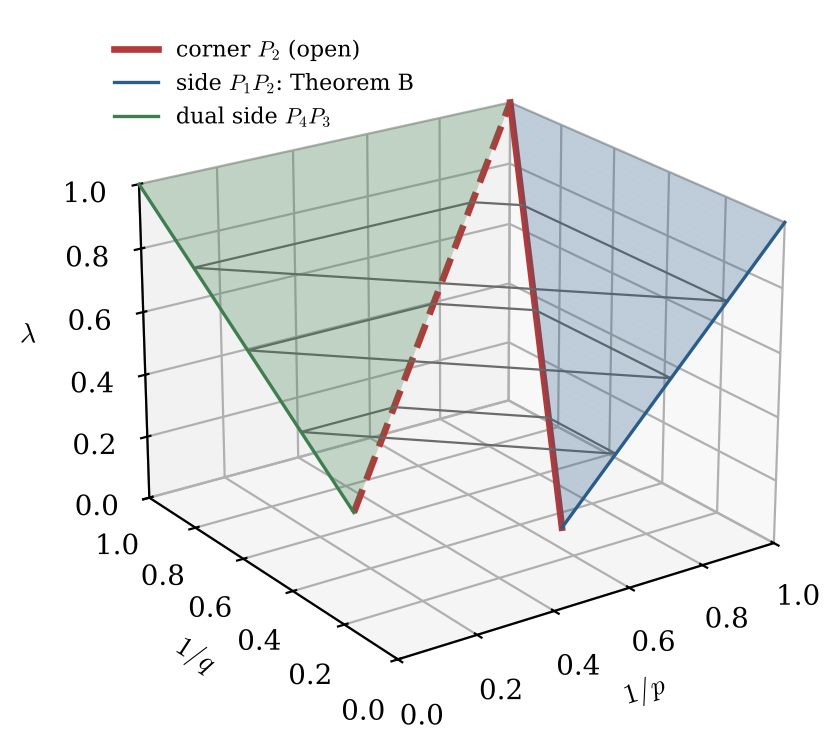
\includegraphics[width=0.78\textwidth]{figures/fig_sparse.png}
\caption{Sparse exponents $(1/p,1/q)$ for $n=3$ at height $\lambda=\lambda(p)$. The grey quadrilaterals
are the trapezoids $P_1P_2P_3P_4$ of \cite[(1.5)]{BRS25} at $\lambda=\frac14,\frac12,\frac34$. As
$\lambda$ runs over $(0,\frac{n-1}2)$ the critical side $P_1P_2$ sweeps the blue surface, which
Theorem B covers except for the red edge traced by the corner $P_2$, where $q=q_{\rm opt}(p)$; the
green surface and the dashed edge are their duals $P_4P_3$ and $P_3$.}
\label{fig:sparse}
\end{figure}

\subsection{Weights}\label{sec:weights}
A \emph{weight} is a locally integrable function $w>0$ almost everywhere. For a ball $B$ write
$\fint_Bw=|B|^{-1}\int_Bw$ and $w(E)=\int_Ew$. The weight belongs to $A_1$ if
\[
[w]_{A_1}=\sup_B\Bigl(\fint_Bw\Bigr)\Bigl(\operatorname*{ess\,inf}_Bw\Bigr)^{-1}<\infty,
\]
and, for $1<\sigma<\infty$, to $RH_\sigma$ if
\[
[w]_{RH_\sigma}=\sup_B\Bigl(\fint_Bw^\sigma\Bigr)^{1/\sigma}\Bigl(\fint_Bw\Bigr)^{-1}<\infty ,
\]
the suprema over all balls. By H\"older's inequality $RH_\sigma\subset RH_{\tilde\sigma}$ when
$\tilde\sigma<\sigma$. Every $A_1$ weight belongs to $RH_\sigma$ for some $\sigma>1$, by the reverse H\"older
inequality of Coifman and Fefferman \cite{CF74}, and $A_1\subset A_p$ for $p>1$, so the
Hardy--Littlewood maximal operator $M$ is bounded on $L^p(w)$ for $w\in A_1$ and $1<p<\infty$
\cite[Ch.~7]{Gra14}. The weak space $L^{p,\infty}(w)$ has the quasinorm
$\|f\|_{L^{p,\infty}(w)}=\sup_{s>0}s\,w(\{|f|>s\})^{1/p}$, which satisfies
$\|f+g\|_{L^{p,\infty}(w)}\le2(\|f\|_{L^{p,\infty}(w)}+\|g\|_{L^{p,\infty}(w)})$ and
$\|f\|_{L^{p,\infty}(w)}\le\|f\|_{L^p(w)}$, and $L^{p,\infty}(w)$ is complete.

\begin{theorem}[{\cite[Theorem 1.4]{FN19}}]\label{thm:fn}
Let $1\le p<q'$, so that $\frac1p+\frac1q>1$, and put $\sigma=(q'/p)'=\frac q{q+p-pq}$. There is a
function $\Phi$, increasing in each variable, such that every $T\in\Sp(p,q)$ satisfies
\[
\|Tf\|_{L^{p,\infty}(w)}\le\Phi\bigl([w]_{A_1},[w]_{RH_\sigma}\bigr)\,\|T\|_{\Sp(p,q)}\|f\|_{L^p(w)}
\qquad(f\in C^\infty_c(\R^n))
\]
for every $w\in A_1\cap RH_\sigma$.
\end{theorem}

This is \cite[Theorem 1.4]{FN19} in the notation of \cite[(9.2)]{BRS25}, where the constant is,
up to a factor depending on $n,p,q$,
\[
\|T\|_{\Sp(p,q)}[w^\sigma]_{A_\infty}^{1/p}[w]_{A_1}^{1+1/p}[w]_{RH_\sigma}^{1/p},
\]
and $[v]_{A_\infty}=\sup_Bv(B)^{-1}\int_BM(v\mathbf 1_B)$ is Wilson's constant. It is bounded by
a function of $[w]_{A_1}$ and $[w]_{RH_\sigma}$: for every ball,
\[
\fint_Bw^\sigma\le[w]_{RH_\sigma}^\sigma\Bigl(\fint_Bw\Bigr)^\sigma\le([w]_{RH_\sigma}[w]_{A_1})^\sigma
\operatorname*{ess\,inf}_Bw^\sigma ,
\]
so $v=w^\sigma\in A_1$ with $[v]_{A_1}\le([w]_{RH_\sigma}[w]_{A_1})^\sigma$; then $Mv\le[v]_{A_1}v$ almost
everywhere, for $M$ the maximal operator over balls containing the point, and
$[v]_{A_\infty}\le[v]_{A_1}$.

\subsection{Proof of Theorem C}\label{ssec:proofC}
Let $w\in A_1\cap RH_\sigma$ with $\sigma>1$, and $1<p<p_1(w)=1+\frac{n-1}{n+1}(1-\frac1\sigma)$. Then
$p<\frac{2n}{n+1}$. For $q\in(q_{\rm opt}(p),p')$ put $\sigma(q)=\frac q{q+p-pq}$, the exponent of Theorem
\ref{thm:fn}. The interval is not empty: $q_{\rm opt}(p)<p'$ is equivalent to
$(n-1)(p-1)<n+1-2p$, that is to $p<\frac{2n}{n+1}$. On it the denominator
$q+p-pq=q\bigl(1-p(1-\frac1q)\bigr)$ is positive, since $1-\frac1q<\frac1p$, and
$\sigma(q)=\bigl(1+\frac pq-p\bigr)^{-1}$ is continuous and increasing in $q$. At $q=q_{\rm opt}(p)$,
\[
q+p-pq=\frac{(n-1)p(1-p)+p(n+1-2p)}{n+1-2p}=\frac{p\,(2n-(n+1)p)}{n+1-2p},
\]
so that
\[
\sigma(q_{\rm opt}(p))=\frac{n-1}{2n-(n+1)p} .
\]
The hypothesis $p<p_1(w)$ is equivalent to $(n+1)p<2n-\frac{n-1}\sigma$, that is to
$\sigma(q_{\rm opt}(p))<\sigma$. By continuity there is $q\in(q_{\rm opt}(p),p')$ with $\sigma(q)<\sigma$,
and then $w\in RH_{\sigma(q)}$.

For this $q$, Theorem B gives $\|R^{\lambda(p)}_{a,t}\|_{\Sp(p,q)}\le C$ with $C$ independent of $t$, and
Theorem \ref{thm:fn} gives
\begin{equation}\label{eq:weightedweak}
\|R^{\lambda(p)}_{a,t}f\|_{L^{p,\infty}(w)}\le C\,\Phi\bigl([w]_{A_1},[w]_{RH_{\sigma(q)}}\bigr)\|f\|_{L^p(w)}
\qquad(f\in C^\infty_c(\R^n),\ t>0).
\end{equation}
The functions $C^\infty_c$ are dense in $L^p(w)$: continuous functions with compact support are
dense since $w\,dx$ is a Radon measure \cite[Theorem 3.14]{Rud87}, and a mollification of such a
function converges uniformly with supports in a fixed compact set, hence in $L^p(w)$ because
$w\in L^1_{\rm loc}$. As $L^{p,\infty}(w)$ is complete, $R^{\lambda(p)}_{a,t}$ extends uniquely to a
bounded operator $L^p(w)\to L^{p,\infty}(w)$ satisfying \eqref{eq:weightedweak}, uniformly in $t$.

\emph{Convergence.} Let $\mathcal G$ be the set of $g\in\mathcal S(\R^n)$ with $\hat g\in C^\infty_c(\R^n\setminus\{0\})$.
We first show that $\mathcal G$ is dense in $L^p(w)$. Fix $\varphi_0\in C^\infty_c(\R^n)$ with
$\varphi_0=1$ on $\{|\xi|\le1\}$, let $\phi=\mathcal F^{-1}\varphi_0\in\mathcal S$, so that $\int\phi=1$, and
for $g\in C^\infty_c$ and $k\ge1$ let $\hat g_k(\xi)=(\varphi_0(\xi/k)-\varphi_0(k\xi))\hat g(\xi)$. Then
$\hat g_k$ is smooth with compact support and vanishes on $\{|\xi|<1/k\}$, so $g_k\in\mathcal G$, and
$g-g_k=g-\phi_{1/k}*g+\phi_k*g$ with $\phi_\eps(x)=\eps^{-n}\phi(x/\eps)$. Both $|\phi_{1/k}*g|$ and
$|\phi_k*g|$ are at most $C_\phi Mg$, with $C_\phi=\int\sup_{|y|\ge|x|}|\phi(y)|\,dx$ \cite[Theorem 2.1.10]{Gra14}, and $Mg\in L^p(w)$. Moreover $\phi_{1/k}*g\to g$ and
$|\phi_k*g|\le k^{-n}\|\phi\|_\infty\|g\|_1\to0$ pointwise. Dominated convergence gives
$g_k\to g$ in $L^p(w)$, and density of $C^\infty_c$ gives density of $\mathcal G$.

For $g\in\mathcal G$ choose $0<\rho_1<\rho_2$ with $\supp\hat g\subset\{\rho_1\le|\xi|\le\rho_2\}$. For
$t\ge2\rho_2$ the function $h_t=R^{\lambda(p)}_{a,t}g-g$ has
$\hat h_t(\xi)=\bigl((1-|\xi/t|^a)^{\lambda(p)}-1\bigr)\hat g(\xi)$, and on
$\{\rho_1\le|\xi|\le\rho_2\}$ we have $|\xi/t|^a\le2^{-a}$. There the map
$s\mapsto(1-s)^{\lambda(p)}-1$ is smooth on $[0,2^{-a}]$ and vanishes at $s=0$, and every derivative of
$\xi\mapsto|\xi/t|^a=t^{-a}|\xi|^a$ is $O(t^{-a})$ uniformly on the annulus. Hence
$\|\partial^\beta\hat h_t\|_\infty\le C_\beta t^{-a}$ for every multi-index $\beta$, with $\hat h_t$
supported in a fixed compact set, and integration by parts gives
$|h_t(x)|\le C_Nt^{-a}(1+|x|)^{-N}$ for every $N$. Now let $c_1=\operatorname{ess\,inf}_{B(0,1)}w$. For
$\varrho\ge1$ the $A_1$ condition on $B(0,\varrho)\supset B(0,1)$ gives
$w(B(0,\varrho))\le[w]_{A_1}c_1|B(0,\varrho)|$, so with $Np>n$,
\[
\int(1+|x|)^{-Np}w(x)\,dx\le w(B(0,1))+\sum_{k\ge0}2^{-kNp}w(B(0,2^{k+1}))\le C\sum_{k\ge0}2^{-kNp+kn}<\infty .
\]
Therefore $\|h_t\|_{L^p(w)}\le Ct^{-a}\to0$ as $t\to\infty$.

Finally let $f\in L^p(w)$ and $\eps>0$. Choose $g\in\mathcal G$ with $\|f-g\|_{L^p(w)}\le\eps$. With $C_w$
the constant of \eqref{eq:weightedweak},
\begin{align*}
\|R^{\lambda(p)}_{a,t}f-f\|_{L^{p,\infty}(w)}
&\le4\|R^{\lambda(p)}_{a,t}(f-g)\|_{L^{p,\infty}(w)}+4\|h_t\|_{L^{p,\infty}(w)}+2\|g-f\|_{L^{p,\infty}(w)}\\
&\le(4C_w+2)\eps+4\|h_t\|_{L^p(w)},
\end{align*}
and the last term tends to zero. Hence $R^{\lambda(p)}_{a,t}f\to f$ in $L^{p,\infty}(w)$. \qed

\subsection{Proof of Theorem A}\label{ssec:proofA}
The weight $w\equiv1$ has $[w]_{A_1}=1$ and $[w]_{RH_\sigma}=1$ for every $\sigma>1$. Given
$1<p<\frac{2n}{n+1}$, choose $\sigma>1$ so large that
$p<1+\frac{n-1}{n+1}(1-\frac1\sigma)$; this is possible because the right side tends to
$\frac{2n}{n+1}$ as $\sigma\to\infty$. Theorem C with this weight is Theorem A. \qed

\begin{remark}\label{rem:wherenew}
For $n=2$ the inputs of Theorems A--C were known before \cite{OAI26}: the Bochner--Riesz conjecture in
the plane \cite{CS72} gives the hypothesis of Theorem \ref{thm:vbr} for every $p_\circ<\frac43$. For
$n\ge3$, \cite{BRS25} proves these conclusions in partial ranges, unconditionally where the
Stein--Tomas theorem suffices; for the weights this is $\sigma\le\frac{n+3}2$, which gives $p<p_{\rm ST}$.
The full ranges rest on Theorem \ref{thm:BR} for every $p_\circ<\frac{2n}{n+1}$.
\end{remark}

\section{The weighted range at its right end}\label{sec:boundary}

Theorem C is stated for $p<p_1(w)$, an open condition in $p$ for a fixed exponent $\sigma$. This
section shows that the end point $p=p_1(w)$ is included as well, because the reverse H\"older
exponent of an $A_1$ weight can always be raised. The argument is the classical self-improvement
of reverse H\"older inequalities \cite{CF74}, written out with explicit constants; it uses
nothing about Bochner--Riesz means beyond Theorem C, and adds nothing at the corner $P_2$ of
Theorem B.

In this section cubes have sides parallel to the axes. Let $\omega_n=|B(0,1)|$ and
\[
\kappa_n=\frac{\omega_n n^{n/2}}{2^n},\qquad \mu_n=\frac{2^n}{\omega_n},
\]
the ratio of the volume of a ball to that of the cube inscribed in it, and of a cube to that of
the ball inscribed in it.

\begin{lemma}\label{lem:gehring}
Let $v$ be a weight and $K\ge1$ with $\fint_Qv\le K\operatorname*{ess\,inf}_Qv$ for every cube $Q$. Then
for $0<\eta\le(2^{n+1}K)^{-1}$ and every cube $Q$,
\[
\fint_Qv^{1+\eta}\le2\Bigl(\fint_Qv\Bigr)^{1+\eta}.
\]
\end{lemma}

\begin{proof}
Fix $Q$ and put $b=\fint_Qv>0$. For $x\in Q$ let $M_Qv(x)$ be the supremum of $\fint_Pv$ over the
dyadic subcubes $P$ of $Q$ containing $x$. Then $M_Qv\ge b$ on $Q$, and $v\le M_Qv$ almost
everywhere on $Q$ by the Lebesgue differentiation theorem along dyadic cubes. For each dyadic
subcube $P$ the hypothesis gives $\fint_Pv\le Kv(x)$ for almost every $x\in P$; as there are
countably many such $P$, $M_Qv\le Kv$ almost everywhere on $Q$.

For $\lambda\ge b$ let $\Omega_\lambda=\{x\in Q:M_Qv(x)>\lambda\}$. It is the disjoint union of the
maximal dyadic subcubes $Q_j$ of $Q$ with $\fint_{Q_j}v>\lambda$. None of them is $Q$, since
$\fint_Qv=b\le\lambda$, and by maximality the parent $\widehat Q_j$ of $Q_j$ has
$\fint_{\widehat Q_j}v\le\lambda$. Hence
\begin{equation}\label{eq:gehringlevel}
v(\Omega_\lambda)=\sum_j\int_{Q_j}v\le\sum_j\int_{\widehat Q_j}v\le2^n\lambda\sum_j|Q_j|
=2^n\lambda|\Omega_\lambda|.
\end{equation}

Let $L\ge b$, $F=\min\{M_Qv,L\}$ and $I=\int_QF^\eta v\le L^\eta v(Q)<\infty$. On $Q$ we have
$F\ge b$, and for $b\le\lambda<L$ the set $\{F>\lambda\}$ is $\Omega_\lambda$. The layer-cake
formula and \eqref{eq:gehringlevel} give
\begin{align*}
I&=\int_0^b\eta\lambda^{\eta-1}v(Q)\,d\lambda+\int_b^L\eta\lambda^{\eta-1}v(\Omega_\lambda)\,d\lambda
\le b^\eta v(Q)+2^n\eta\int_0^\infty\lambda^\eta\bigl|\{x\in Q:F(x)>\lambda\}\bigr|\,d\lambda\\
&=b^\eta v(Q)+\frac{2^n\eta}{1+\eta}\int_QF^{1+\eta}
\le b^\eta v(Q)+2^nK\eta\, I,
\end{align*}
since $F^{1+\eta}=F^\eta F\le KF^\eta v$. As $2^nK\eta\le\frac12$ and $I$ is finite,
$I\le2b^\eta v(Q)$. Letting $L\to\infty$, monotone convergence and $v\le M_Qv$ give
$\int_Qv^{1+\eta}\le\int_Q(M_Qv)^\eta v\le2b^\eta v(Q)=2b^{1+\eta}|Q|$.
\end{proof}

\begin{proposition}\label{prop:selfimprove}
Let $\sigma>1$, $w\in A_1\cap RH_\sigma$, $A=[w]_{A_1}$, $B=[w]_{RH_\sigma}$, and
\[
K=\kappa_n(AB)^\sigma,\qquad\eta=\frac1{2^{n+1}K},\qquad\Sigma=\sigma(1+\eta).
\]
Then $w\in RH_\Sigma$ and $[w]_{RH_\Sigma}\le(2\mu_nK^{1+\eta})^{1/\Sigma}B$.
\end{proposition}

\begin{proof}
Put $v=w^\sigma$. For every ball $B'$, as shown after Theorem \ref{thm:fn},
$\fint_{B'}v\le(AB)^\sigma\operatorname*{ess\,inf}_{B'}v$. If $Q$ is a cube and $B'$ the ball circumscribed
about it, then $|B'|=\kappa_n|Q|$ and
\[
\fint_Qv\le\kappa_n\fint_{B'}v\le\kappa_n(AB)^\sigma\operatorname*{ess\,inf}_{B'}v
\le K\operatorname*{ess\,inf}_Qv .
\]
Here $K\ge1$, since $A\ge1$, $B\ge1$ and $\kappa_n\ge1$, so Lemma \ref{lem:gehring} applies to $v$.
Now let $B'$ be a ball and $Q$ the cube circumscribed about it, so $|Q|=\mu_n|B'|$. By the lemma
and the bound just proved,
\[
\fint_{B'}v^{1+\eta}\le\mu_n\fint_Qv^{1+\eta}\le2\mu_n\Bigl(\fint_Qv\Bigr)^{1+\eta}
\le2\mu_n\bigl(K\operatorname*{ess\,inf}_Qv\bigr)^{1+\eta}\le2\mu_nK^{1+\eta}\Bigl(\fint_{B'}v\Bigr)^{1+\eta},
\]
since $\operatorname*{ess\,inf}_Qv\le\operatorname*{ess\,inf}_{B'}v\le\fint_{B'}v$. With $v=w^\sigma$ and
$\fint_{B'}w^\sigma\le B^\sigma(\fint_{B'}w)^\sigma$ this reads
$\fint_{B'}w^\Sigma\le2\mu_nK^{1+\eta}B^\Sigma(\fint_{B'}w)^\Sigma$.
\end{proof}

\begin{theorem}\label{thm:boundary}
Let $n\ge2$, $a>0$, $\sigma>1$ and $w\in A_1\cap RH_\sigma$, and let $\Sigma>\sigma$ be the exponent of
Proposition \ref{prop:selfimprove}. Then the conclusions of Theorem C hold for
\[
1<p<1+\frac{n-1}{n+1}\Bigl(1-\frac1\Sigma\Bigr),
\]
and in particular at $p=p_1(w)=1+\frac{n-1}{n+1}(1-\frac1\sigma)$. Equivalently, with
$\sigma_w=\sup\{s>1:w\in RH_s\}\in(1,\infty]$, they hold for
$1<p<1+\frac{n-1}{n+1}(1-\frac1{\sigma_w})$, and $w\notin RH_{\sigma_w}$ when $\sigma_w<\infty$.
\end{theorem}

\begin{proof}
By Proposition \ref{prop:selfimprove}, $w\in A_1\cap RH_\Sigma$, and Theorem C with $\Sigma$ in place
of $\sigma$ gives the first assertion; since $s\mapsto1-\frac1s$ is increasing and $\Sigma>\sigma$,
the range contains $p_1(w)$. The set of $s>1$ with $w\in RH_s$ is an interval by H\"older's
inequality, nonempty by \cite{CF74}, and open by Proposition \ref{prop:selfimprove}; so its
supremum $\sigma_w$ is not attained, and every $p<1+\frac{n-1}{n+1}(1-\frac1{\sigma_w})$ is below
$p_1$ for some admissible exponent.
\end{proof}

\begin{corollary}\label{cor:A1only}
Let $n\ge2$, $a>0$ and $w\in A_1$. The conclusions of Theorem C hold for
\[
1<p<1+\frac{n-1}{(n+1)\bigl(2^{n+1}\kappa_n[w]_{A_1}+1\bigr)} .
\]
\end{corollary}

\begin{proof}
The second half of the proof of Proposition \ref{prop:selfimprove}, applied to $v=w$ with
$K=\kappa_n[w]_{A_1}$ in place of $\kappa_n(AB)^\sigma$, shows that $w\in RH_{1+\eta_0}$ with
$\eta_0=(2^{n+1}\kappa_n[w]_{A_1})^{-1}$. Theorem C with
$\sigma=1+\eta_0$ gives the range, since $1-\frac1{1+\eta_0}=\frac{\eta_0}{1+\eta_0}
=\frac1{2^{n+1}\kappa_n[w]_{A_1}+1}$.
\end{proof}

\begin{example}\label{ex:powerweight}
For $0\le\beta<n$ the weight $|x|^{-\beta}$ lies in $A_1$ \cite[\S7.1]{Gra14}. Let $0\le\gamma<n$ and
$w(x)=|x|^{-\gamma}$. If $\gamma s<n$, then $w^s\in A_1$, so
$\fint_Bw^s\le C\operatorname*{ess\,inf}_Bw^s\le C(\fint_Bw)^s$ for every ball and $w\in RH_s$; if
$\gamma s\ge n$, then $w^s$ is not integrable near $0$ and $w\notin RH_s$. Thus $\sigma_w=n/\gamma$, and
Theorem \ref{thm:boundary} gives the weak-type bound on $L^p(|x|^{-\gamma})$ for
\[
1<p<1+\frac{n-1}{n+1}\Bigl(1-\frac\gamma n\Bigr).
\]
For $\gamma=0$ this is Theorem A.
\end{example}

\section{What remains open}\label{sec:open}

\subsection{The corner of the trapezoid}
Theorem B covers the critical side $P_1P_2$ of the trapezoid of \cite[(1.5)]{BRS25} except the corner
$P_2$, where $q=q_{\rm opt}(p)$. At $P_2$ the scale-by-scale estimates behind Theorem \ref{thm:brs} sum
only with a loss: the exponent $r_*(p,p_\circ)$ reaches the Knapp line $r=\frac{n-1}{n+1}p'$ only in the
limit \eqref{eq:rstarlimit}, and the hypothesis of Theorem \ref{thm:brs} asks for $r<r_*$. The method would
need $\VBR(p,\frac{n-1}{n+1}p')$, the endpoint of the conjectured range of these inequalities, which is
established in \cite{BRS25} only at $p=p_{\rm ST}$. For $p=p_{\rm ST}$ the corner is reached in
\cite[Theorem 1.5]{BRS25}, through the $L^2$ restriction theorem; for $n=2$ the corner is also open
except at $\lambda=\frac16$ \cite[\S1.2]{BRS25}.

\subsection{The other sides}
For $0<\lambda<\frac{n-1}2$, sparse bounds on the top side $P_2P_3$ of the trapezoid, away from the
critical line, are open for $n\ge3$, and in the plane except at $\lambda=\frac16$. They are a
strengthening of off-diagonal $L^p\to L^r$ bounds for Bochner--Riesz means below the critical index,
and Theorem \ref{thm:BR} does not reach them. By duality the side $P_3P_4$ is equivalent to the side
$P_1P_2$, so Theorem B also gives it, except for the corner $P_3$.

\subsection{The range of the weights}
The exponent $p_1(w)=1+\frac{n-1}{n+1}(1-\frac1\sigma)$ of Theorem C is the one produced by Theorem
\ref{thm:fn} from the sparse bounds of Theorem B. Whether it is the sharp range in terms of the reverse
H\"older exponent is not known, as already noted in \cite[\S1.1]{BRS25}; weighted weak-type bounds
fail for $p>1$ for the power weights $|x|^\eps$, $\eps>0$ \cite[\S1.1]{BRS25}, so some restriction of
this kind is necessary.

\subsection{Other domains}
Parts I and II are written for the round sphere. Beltran, Roos and Seeger work with the Minkowski
functional $\rho$ of a convex domain with smooth boundary of positive curvature, and their
Theorem \ref{thm:brs} holds in that generality. The weak-type endpoint for such $\rho$ in dimensions
$n\ge3$ would follow in the same way from the Bochner--Riesz conjecture for $(1-\rho(\xi))^\lambda_+$,
which the local smoothing argument of Part I does not address.

\subsection{Maximal functions}
The maximal operator $\sup_{t>0}|R^{\lambda(p)}_{a,t}f|$ is not treated here. Already for
$\lambda>\lambda(p)$ and $p<2$ its $L^p$ boundedness requires conditions beyond those of the
Bochner--Riesz conjecture \cite{Tao02}, and nothing in this paper bears on it.

\appendix
\section{The Dirichlet problem on a periodic fibre}\label{app:dirichlet}

The energy argument of Section \ref{sec:energy} uses a potential that solves a quaternionic
Monge--Amp\`ere equation on each spatial fibre, is smooth up to a boundary that moves with the
parameters, and is compared with explicit functions on the fibre and on small balls inside it. This
appendix proves the existence, comparison and smooth dependence that are needed; the quantitative
bounds in the wavelength come from the comparison functions of Section \ref{sec:fiber}. The argument
is that of \cite[Appendix A]{OAI26}, written out in full. Alesker solved the Dirichlet problem on
quaternionic balls \cite[Theorem 1.4]{Ale03b} and Zhu on bounded domains of $\HH^m$ carrying a smooth
subsolution \cite[Theorem 1.1]{Zhu16}. Our fibres have periodic real directions and only three real
coordinates per variable; a fourth, periodic coordinate is adjoined to provide the quaternionic
rotations used for the mixed derivatives at the boundary.

\subsection{Setting and statement}
Let $m\ge1$, let $\Lambda\subset\R^m$ be a lattice of rank $m$, let $V\subset\Ck^m\cong\R^{2m}$ be a bounded
domain with smooth boundary, and put $\Omega=(\R^m/\Lambda)\times V$. In the notation of Section
\ref{ssec:hessian} with three slots, $z_a=x_a+P_a\ii$, the periodic variables $x_a$ occupy the real
slot and $P_a=p_a+\kk q_a\in\Ck$ the slots $\ii,\jj$; $H$ is the three-slot Hessian \eqref{eq:GH}. A
function on $V$ is regarded as a function on $\Omega$ independent of $x$.

\begin{theorem}[{\cite[Theorem A.1]{OAI26}}]\label{thm:dirichlet}
Let $r$ be smooth on a neighbourhood of $\overline V$, with $r<0$ in $V$, $r=0$ and $dr\ne0$ on
$\partial V$, and $H(r)>0$ on $\overline\Omega$. Let $B_0,g\in C^\infty(\overline\Omega)$ be real with
\[
H(B_0)\ge0,\qquad g>\det H(B_0)\qquad\text{on }\overline\Omega .
\]
Then there is a unique $u\in C^\infty(\overline\Omega)$ with
\begin{equation}\label{eq:dirichletA}
\det H(B_0+u)=g,\qquad H(B_0+u)>0\quad\text{on }\overline\Omega,\qquad u|_{\partial\Omega}=0,
\end{equation}
and there are constants $b\ge b'>0$ with
\begin{equation}\label{eq:barrier}
b\,r\le u\le b'\,r .
\end{equation}
If $r,B_0,g$ and the domain depend smoothly on finitely many parameters, the constants $b,b'$ can be
chosen locally uniformly in the parameters, and the solution depends smoothly on the parameters up to
the boundary after any smooth local identification of the domains with a fixed domain.
\end{theorem}

Here $C^\infty(\overline\Omega)$ denotes functions all of whose derivatives extend continuously to
$\overline\Omega$, and similarly for the H\"older spaces $C^{k,\alpha}(\overline\Omega)$; $C^{k,\alpha}_0$ is
the subspace of functions vanishing on $\partial\Omega$. The \emph{smooth dependence} means: if
$\Theta_\tau:\overline V_{\tau_0}\to\overline V_\tau$ are diffeomorphisms depending smoothly on $(\tau,y)$, then
$(\tau,x,y)\mapsto u_\tau(x,\Theta_\tau(y))$ is smooth up to the boundary.

\subsection{Matrix facts}
We use the following consequences of Lemma \ref{lem:moore}. Let $Q,Q_1,Q_2$ be positive definite
Hermitian quaternionic $m\times m$ matrices and $B$ Hermitian.
\begin{enumerate}[label=(M\arabic*)]
\item If $A\ge0$ and $B\ge0$ then $A:B\ge0$. Indeed $A=UDU^*$ with $U$ unitary and $D\ge0$ diagonal, and
$A:B=\Re\tr(D^{1/2}U^*BUD^{1/2})$ by cyclicity of $\Re\tr$, a sum of the nonnegative numbers
$e_i^*D^{1/2}U^*BUD^{1/2}e_i$.
\item $\frac{d}{ds}\log\det(Q+sB)|_{s=0}=Q^{-1}:B$, by \eqref{eq:cofactor} and \eqref{eq:cofinv}. Since
$Q_\theta=(1-\theta)Q_2+\theta Q_1>0$ for $0\le\theta\le1$,
\begin{equation}\label{eq:logdiff}
\log\det Q_1-\log\det Q_2=\Bigl(\int_0^1Q_\theta^{-1}\,d\theta\Bigr):(Q_1-Q_2).
\end{equation}
\item Put $S=\Re\tr Q^{-1}$, the sum of the reciprocals of the eigenvalues of $Q$. By the
arithmetic--geometric mean inequality $S\ge m(\det Q)^{-1/m}$. If $-\beta I\le B\le\beta I$ then
$|Q^{-1}:B|\le\beta S$, by (M1) applied to $\beta I\pm B$.
\item If $A\ge0$ and $P\ge cI$ with $c>0$, then $\det(A+P)>\det A$. Indeed the real representation
\eqref{eq:realrep} turns $A$ and $A+P$ into symmetric real matrices with $(A+P)_{\R}\ge A_{\R}+cI$, so by the
minimax characterisation each eigenvalue of $(A+P)_{\R}$ exceeds the corresponding eigenvalue of $A_{\R}$
by at least $c$, and \eqref{eq:realrep} gives $\det(A+P)^4>\det(A)^4\ge0$.
\end{enumerate}

\subsection{The linearised operator and comparison}
Work with $k\in\{3,4\}$ slots and $m$ coordinate indices; the real dimension is $N=km$, and $H$ is the
$k$-slot Hessian. For a real covector $\xi\in\R^N$ write $\hat\xi=(\sum_\alpha e_\alpha\xi_{a\alpha})_a\in\HH^m$;
then $|\hat\xi|=|\xi|$. For a real symmetric $N\times N$ matrix $M$ let $H(M)$ be the Hermitian matrix with
$H(D^2v)=H(v)$; it is linear in $M$, and $H(\xi\xi^{\rm t})=\hat\xi\hat\xi^*$ by Lemma \ref{lem:hessian}. If
$Q>0$ is a Hermitian matrix field, the operator
\[
L_Qw=Q^{-1}:H(w)
\]
is a real linear operator $\sum_{i,j}a^{ij}\partial_i\partial_jw$ with no lower-order terms, whose coefficient
matrix is defined by $a:M=Q^{-1}:H(M)$. For $M=\xi\xi^{\rm t}$ this gives
$a(\xi,\xi)=\hat\xi^*Q^{-1}\hat\xi$, so
\begin{equation}\label{eq:ellipticity}
\lambda_{\max}(Q)^{-1}|\xi|^2\le a(\xi,\xi)\le\lambda_{\min}(Q)^{-1}|\xi|^2 .
\end{equation}
If $\psi$ is a $C^2$ function with $Q=H(\psi)>0$ we write $L_\psi=L_{H(\psi)}$, the derivative of
$\psi\mapsto\log\det H(\psi)$ by (M2).

In what follows a \emph{periodic domain} is an open set $U\subset(\R^{m}/\Lambda)\times W$, where $W$ is
bounded in the remaining real coordinates and $\Lambda$ is a lattice (possibly of lower rank, possibly
acting on more coordinates), so that $\overline U$ is compact and at least one real coordinate $y$ is
a bounded function on $U$. The domain $\Omega$, its four-slot extension below, and balls in a
fibre are periodic domains.

\begin{lemma}[Maximum principle]\label{lem:maxprinciple}
Let $U$ be a periodic domain and $L=\sum a^{ij}\partial_i\partial_j$ with $a$ continuous and positive
definite in $U$. If $f\in C^2(U)\cap C(\overline U)$ satisfies $Lf\ge0$ in $U$, then
$\max_{\overline U}f=\max_{\partial U}f$.
\end{lemma}

\begin{proof}
At an interior maximum $D^2f\le0$, so $Lf=a:D^2f\le0$; hence a function with $Lf>0$ has no interior
maximum. Let $y$ be a bounded real coordinate and $h=e^{y}$. Then $Lh=a^{yy}e^y>0$, so
for $\eps>0$ the function $f+\eps h$ satisfies $L(f+\eps h)>0$ and attains its maximum over the
compact set $\overline U$ on $\partial U$. Letting $\eps\to0$ gives the claim.
\end{proof}

\begin{lemma}[Comparison]\label{lem:comparison2}
Let $U$ be a periodic domain in $k$ slots, and $\psi_1,\psi_2\in C^2(U)\cap C(\overline U)$ with
$H(\psi_i)>0$ in $U$. If $\det H(\psi_1)\ge\det H(\psi_2)$ in $U$ and $\psi_1\le\psi_2$ on $\partial U$,
then $\psi_1\le\psi_2$ in $U$. In particular \eqref{eq:dirichletA} has at most one solution in
$C^2(\Omega)\cap C(\overline\Omega)$.
\end{lemma}

\begin{proof}
By \eqref{eq:logdiff}, $0\le\log\det H(\psi_1)-\log\det H(\psi_2)=L_{\bar Q}(\psi_1-\psi_2)$ with
$\bar Q^{-1}=\int_0^1Q_\theta^{-1}d\theta$, $Q_\theta=(1-\theta)H(\psi_2)+\theta H(\psi_1)$. The coefficients
are continuous and positive definite in $U$ by \eqref{eq:ellipticity}, and Lemma \ref{lem:maxprinciple}
gives $\psi_1-\psi_2\le\max_{\partial U}(\psi_1-\psi_2)\le0$. For uniqueness apply this twice with
$\psi_i=B_0+u_i$.
\end{proof}

\subsection{The four-slot extension}
Let $\tilde\Omega=\Omega\times(\R/\Z)^m$, with the new coordinates $z_{a3}$ in the $\kk$ slots, and extend
$r,B_0,g$ to $\tilde\Omega$ as functions independent of them. For a function independent of the $\kk$
slots the four-slot $G$ and $H$ of \eqref{eq:GH} agree with the three-slot ones, since every term
containing $\partial_{a3}$ vanishes. Hence the hypotheses of Theorem \ref{thm:dirichlet} hold on
$\tilde\Omega$, and a solution on $\Omega$ extends to a solution on $\tilde\Omega$. Conversely, suppose
$\tilde u$ solves the four-slot problem on $\tilde\Omega$. For $c\in(\R/\Z)^m$ the translate
$\tilde u(\cdot+c)$ in the $\kk$ slots solves the same problem, since the data are invariant and
$H$ commutes with translations. By Lemma \ref{lem:comparison2} (with $k=4$), $\tilde u(\cdot+c)=\tilde u$,
so $\tilde u$ is independent of the $\kk$ slots and restricts to a solution on $\Omega$. Therefore it
suffices to prove Theorem \ref{thm:dirichlet} on $\tilde\Omega$, and the rest of the proof works there,
with four slots and $N=4m$.

The manifold $\overline{\tilde\Omega}$ is compact with smooth boundary
$\partial\tilde\Omega=(\R^m/\Lambda)\times\partial V\times(\R/\Z)^m$ and a flat metric, and each point has a
neighbourhood isometric to an open subset of $\R^{4m}$ in which the boundary is a smooth hypersurface.
We call such a neighbourhood a \emph{flat chart}. By compactness $\overline{\tilde\Omega}$ is covered by
finitely many flat charts of a fixed size. The local Schauder estimates \cite[Corollary 6.3 and Lemma
6.5]{GT01}, their higher-order forms, and the local $L^2$ regularity \cite[Theorems 8.8 and 8.12]{GT01}
are local statements and apply in such charts; summing over a finite cover gives the global estimates
of \cite[Theorem 6.6]{GT01} and their higher-order analogues on $\overline{\tilde\Omega}$, exactly as in
the proofs in \cite[Ch.~6]{GT01}.

\subsection{The linear Dirichlet problem}
\begin{lemma}\label{lem:lineardirichlet}
Let $Q>0$ be a smooth Hermitian field on $\overline{\tilde\Omega}$, $k\ge0$ and $0<\alpha<1$. Then
$L_Q:C^{k+2,\alpha}_0(\overline{\tilde\Omega})\to C^{k,\alpha}(\overline{\tilde\Omega})$ is an isomorphism.
\end{lemma}

\begin{proof}
For the Laplacian: by Poincar\'e's inequality along a bounded coordinate of $V$, the form
$\int\nabla v\cdot\nabla w$ is coercive on $H^1_0(\tilde\Omega)$, so for $f\in C^\infty(\overline{\tilde\Omega})$ the
Lax--Milgram theorem gives a weak solution $v\in H^1_0$ of $\Delta v=f$. The local regularity theorems,
interior and at the flat boundary pieces, give $v\in H^j$ for every $j$, hence
$v\in C^\infty(\overline{\tilde\Omega})$ by Sobolev embedding. For $f\in C^{k,\alpha}$ mollify in charts to get
smooth $f_\ell$ bounded in $C^{k,\alpha}$ and converging in $C^{k,\beta}$, $\beta<\alpha$. The estimate
below bounds the solutions $v_\ell$ in $C^{k+2,\alpha}$; they converge in $C^{k+2,\beta}$, and the limit
lies in $C^{k+2,\alpha}_0$ and solves $\Delta v=f$. Uniqueness follows from Lemma \ref{lem:maxprinciple}.

For $L_s=(1-s)\Delta+sL_Q$, $0\le s\le1$, the coefficients are smooth and uniformly elliptic,
uniformly in $s$, since $\Delta=L_I$ by Lemma \ref{lem:hessian}. Since $H(r)\ge c_rI$ on
$\overline{\tilde\Omega}$ for some $c_r>0$, (M1) gives $L_sr\ge c'>0$ uniformly in $s$. If
$v\in C^2_0$ and $|L_sv|\le K$, then $L_s(\pm v+\frac K{c'}r)\ge0$ and Lemma \ref{lem:maxprinciple} gives
$|v|\le\frac K{c'}|r|$. With the global Schauder estimate
$\|v\|_{C^{k+2,\alpha}}\le C(\|v\|_{C^0}+\|L_sv\|_{C^{k,\alpha}})$ this gives
$\|v\|_{C^{k+2,\alpha}}\le C\|L_sv\|_{C^{k,\alpha}}$ on $C^{k+2,\alpha}_0$, uniformly in $s$, and the method of
continuity \cite[Theorem 5.2]{GT01} transfers invertibility from $L_0=\Delta$ to $L_1=L_Q$.
\end{proof}

\subsection{The continuity path}
Write $\psi=B_0+u$, so that \eqref{eq:dirichletA} reads $\det H(\psi)=g$, $H(\psi)>0$,
$\psi=B_0$ on $\partial\tilde\Omega$. For $0\le t\le1$ put
\[
g_t=(1-t)\det H(B_0+r)+tg .
\]
At $t=0$ the function $u=r$ is a solution: $H(B_0+r)\ge H(r)>0$ and $r=0$ on the boundary. By (M4),
$\det H(B_0+r)>\det H(B_0)$, and $g>\det H(B_0)$ by hypothesis; by compactness there are
$\delta,c_0,C_0>0$ with
\begin{equation}\label{eq:gap}
g_t\ge\det H(B_0)+\delta,\qquad c_0\le g_t\le C_0\qquad\text{on }\overline{\tilde\Omega},\ 0\le t\le1 .
\end{equation}
Let $T$ be the set of $t\in[0,1]$ for which \eqref{eq:dirichletA} with $g_t$ in place of $g$ has a
solution $u_t\in C^\infty(\overline{\tilde\Omega})$. Then $0\in T$, and we show that $T$ is open and closed.

\emph{Openness.} Let $t_0\in T$, fix $\alpha\in(0,1)$ and $k\ge0$, and consider
\[
\mathcal F(t,u)=\log\det H(B_0+u)-\log g_t
\]
on the open set of $u\in C^{k+2,\alpha}_0$ with $H(B_0+u)>0$ on $\overline{\tilde\Omega}$, with values in
$C^{k,\alpha}$. It is a smooth map: $\log\det H(M)$ is a smooth function of the real Hessian $M$ on the
open set $H(M)>0$, and composition with a smooth function is a smooth map of H\"older spaces. Its
derivative in $u$ at $u_{t_0}$ is $L_{\psi_{t_0}}$, an isomorphism by Lemma
\ref{lem:lineardirichlet}. The implicit function theorem gives, for $t$ near $t_0$, a solution
$u_t\in C^{k+2,\alpha}_0$ depending smoothly on $t$. By Lemma \ref{lem:comparison2} the solutions obtained
for different $k$ coincide, so $u_t\in C^\infty(\overline{\tilde\Omega})$ and $T$ is open.

\emph{Closedness.} By the a priori estimates below, every $u_t$, $t\in T$, satisfies
$\|u_t\|_{C^j(\overline{\tilde\Omega})}\le C_j$ for every $j$, and $H(B_0+u_t)\ge c\,I$, with $C_j,c$
independent of $t$. If $t_\ell\in T$ and $t_\ell\to t$, the Arzel\`a--Ascoli theorem gives a subsequence of
$u_{t_\ell}$ converging in every $C^j$ to some $u\in C^\infty(\overline{\tilde\Omega})$, which vanishes on the
boundary, satisfies $H(B_0+u)\ge cI$ and $\det H(B_0+u)=g_t$. So $t\in T$.

Hence $T=[0,1]$ and $u=u_1$ solves \eqref{eq:dirichletA}. It remains to prove the a priori estimates.
For the rest of this appendix $u=u_t$ is a smooth solution for some $t\in T$, $\psi=B_0+u$,
$Q=H(\psi)$, $L=L_\psi$, $S=\Re\tr Q^{-1}$, and $C$ denotes constants independent of $t$ and $u$.
By (M3) and \eqref{eq:gap},
\begin{equation}\label{eq:Slow}
S\ge m\,g_t^{-1/m}\ge mC_0^{-1/m}=:s_0>0,\qquad Lr=Q^{-1}:H(r)\ge c_rS .
\end{equation}

\subsection{Barriers and the gradient}
\emph{The barriers \eqref{eq:barrier}.} As $b'\downarrow0$, $\det H(B_0+b'r)\to\det H(B_0)$ uniformly, so
by \eqref{eq:gap} we may fix $b'\in(0,1)$ with $\det H(B_0+b'r)<g_t$ for all $t$. Since
$\det H(B_0+br)\ge\det(bH(r))\ge(bc_r)^m$ by (M4) and monotonicity, we may fix $b>1$ with
$\det H(B_0+br)>C_0\ge g_t$. All three potentials $B_0+b'r$, $\psi$, $B_0+br$ equal $B_0$ on the boundary
and have positive definite Hessians, so Lemma \ref{lem:comparison2} gives $B_0+br\le\psi\le B_0+b'r$,
which is \eqref{eq:barrier}. Since $r$ is a defining function, near $\partial\tilde\Omega$ we can write
$u=\rho\,r$ with $\rho$ smooth up to the boundary (Section \ref{ssec:divergence}). On the collar
$r<0$, so \eqref{eq:barrier} gives $b'\le\rho\le b$, and by continuity also on the boundary. There
$\nabla u=\rho\nabla r$, so
\begin{equation}\label{eq:boundarygrad}
|\nabla u|\le b\,|\nabla r|\qquad\text{on }\partial\tilde\Omega .
\end{equation}

\emph{First and second derivatives along constant directions.} For real symmetric $M$ with $H(M)>0$
put $F(M)=\log\det H(M)$. It is concave, being the composition of the linear map $M\mapsto H(M)$ with
the concave function $\log\det$ (Lemma \ref{lem:moore}), and $DF(M)[\dot M]=H(M)^{-1}:H(\dot M)$ by
(M2). For a constant real unit vector $e$ write $\psi_e,\psi_{ee}$ for the directional derivatives.
Differentiating $F(D^2\psi)=\log g_t$ once and twice along $e$ gives
\begin{equation}\label{eq:diffeq}
L\psi_e=(\log g_t)_e,\qquad L\psi_{ee}=(\log g_t)_{ee}-D^2F(D^2\psi)[D^2\psi_e,D^2\psi_e]\ge(\log g_t)_{ee}.
\end{equation}
By \eqref{eq:Slow}, $L(\pm\psi_e+Kr)\ge-C+Kc_rs_0>0$ for a large constant $K$, and Lemma
\ref{lem:maxprinciple} gives $\pm\psi_e\le\max_{\partial\tilde\Omega}|\nabla\psi|+K|r|$. With
\eqref{eq:boundarygrad} this bounds $|\nabla\psi|$, hence $|\nabla u|$, by a constant $C$. In the same
way $L(\psi_{ee}+Kr)>0$ for large $K$, so
\begin{equation}\label{eq:hessreduce}
\psi_{ee}\le\max_{\partial\tilde\Omega}|D^2\psi|+C\qquad\text{in }\tilde\Omega,\ |e|=1 .
\end{equation}
It remains to bound $D^2\psi$ on the boundary; $B_0$ is smooth, so it suffices to bound $D^2u$ there.

\subsection{Second derivatives at the boundary}
Fix a boundary point and a flat chart centred at it, with coordinates $x\in\R^{4m}$, identified with
$\HH^m$ through the slots, so that the real inner product is $\Re(v^*w)$. Let $\nu$ be the outward unit
normal at $0$; then $\nabla r(0)=|\nabla r(0)|\nu$, since $r<0$ inside. All constants below are uniform
over boundary points, by compactness.

\emph{Tangential directions.} From $u=\rho r$,
$D^2u=\rho D^2r+\nabla\rho\otimes\nabla r+\nabla r\otimes\nabla\rho+rD^2\rho$, and at $0$ the last three terms
vanish on pairs of tangent vectors. Hence $|D^2u(0)(v,w)|=\rho|D^2r(0)(v,w)|\le C$ for unit tangent
$v,w$.

\emph{Mixed directions.} Fix a unit tangent vector $e$ at $0$. Let $P_{\rm tan}$ be the real orthogonal
projection onto the tangent space and put
\[
v=\frac{P_{\rm tan}D^2r(0)e}{|\nabla r(0)|},\qquad A=v\nu^*-\nu v^*-\nu(\nu^*v)\nu^* ,
\]
with vectors read as quaternionic columns. Since $v$ is tangent, $\Re(\nu^*v)=0$, so the quaternion
$\nu^*v$ satisfies $\overline{\nu^*v}=-\nu^*v$. Hence
$A^*=\nu v^*-v\nu^*+\nu(\nu^*v)\nu^*=-A$, and, using $\nu^*\nu=1$ and $v^*\nu+\nu^*v=2\Re(\nu^*v)=0$,
\[
A\nu=v-\nu(v^*\nu)-\nu(\nu^*v)=v .
\]
Consider the affine vector field $X(x)=e+Ax$. Its flow is $\phi_s(x)=e^{sA}x+c_s$ with
$c_s=\int_0^se^{\sigma A}e\,d\sigma$, and $U_s=e^{sA}$ is quaternionic unitary since $A^*=-A$.

First, $Xr$ vanishes to second order along the boundary at $0$. Indeed $Xr(0)=\nabla r(0)\cdot e=0$, and
for a tangent vector $w$,
\begin{align*}
\partial_w(Xr)(0)&=D^2r(0)(w,e)+\nabla r(0)\cdot(Aw)
=|\nabla r(0)|\bigl(v\cdot w+\Re(\nu^*Aw)\bigr)\\
&=|\nabla r(0)|\bigl(v\cdot w-\Re((A\nu)^*w)\bigr)=0,
\end{align*}
because $D^2r(0)(w,e)=w\cdot P_{\rm tan}D^2r(0)e$ and $\Re(\nu^*Aw)=\Re((A^*\nu)^*w)=-\Re((A\nu)^*w)$.
So the restriction of $Xr$ to the boundary hypersurface vanishes at $0$ with its differential, and
$|Xr(x)|\le C|x|^2$ for boundary points $x$ in the chart. On the boundary $Xu=\rho\,Xr+r\,X\rho=\rho\,Xr$,
so
\begin{equation}\label{eq:Xuboundary}
|Xu(x)|\le C|x|^2\qquad(x\in\partial\tilde\Omega,\ |x|\le\varrho_0),
\end{equation}
for a fixed chart radius $\varrho_0$.

Secondly, $L(X\psi)=X\log g_t$. By the covariance in Lemma \ref{lem:hessian} and its invariance under
translations, $H(\psi\circ\phi_s)(x)=U_s^*H(\psi)(\phi_s(x))U_s$, and the Moore determinant is invariant
under unitary conjugation, since the eigenvalues are. Hence
$\log\det H(\psi\circ\phi_s)(x)=\log g_t(\phi_s(x))$ for $x$ in the chart and small $s$, and
differentiation at $s=0$, using (M2) and $\frac d{ds}\psi\circ\phi_s|_{s=0}=X\psi$, gives
$L(X\psi)=X\log g_t$. Since $X B_0$ is smooth with $|H(XB_0)|\le C$, (M3) and \eqref{eq:Slow} give
\begin{equation}\label{eq:LXu}
|L(Xu)|\le|X\log g_t|+|L(XB_0)|\le C+CS\le CS .
\end{equation}

Let $U=\{|x|<\varrho_0\}\cap\tilde\Omega$ and $w=K_1|x|^2-K_2r$. On the part of $\partial U$ in the
boundary of $\tilde\Omega$, $w=K_1|x|^2\ge|Xu|$ by \eqref{eq:Xuboundary} once $K_1\ge C$. On the part
where $|x|=\varrho_0$, $w\ge K_1\varrho_0^2\ge|X||\nabla u|\ge|Xu|$ once $K_1$ is large, by the gradient
bound. In four slots $H(|x|^2)=8I$, since $|x|^2=\sum_{a,\alpha}z_{a\alpha}^2$ has real Hessian $2I$ and
each diagonal entry collects $\sum_\alpha e_\alpha\overline{e_\alpha}\cdot2=8$. So by \eqref{eq:Slow} and
\eqref{eq:LXu},
\[
L(w\pm Xu)\le8K_1S-K_2c_rS+CS\le0
\]
once $K_2$ is large. Lemma \ref{lem:maxprinciple} applied to $-(w\pm Xu)$ gives $|Xu|\le w$ in $U$.
At $0$ both $w$ and $Xu=\rho Xr$ vanish. Along the inward normal, $x=-s\nu$ with small $s>0$, we get
$|Xu(-s\nu)|\le K_1s^2-K_2r(-s\nu)\le Cs$, so $|\partial_\nu(Xu)(0)|\le C$. Now
\[
\partial_\nu(Xu)(0)=D^2u(0)(\nu,e)+\nabla u(0)\cdot(A\nu)=D^2u(0)(\nu,e),
\]
because $\nabla u(0)=\rho\nabla r(0)$ is normal and $A\nu=v$ is tangent. Hence $|D^2u(0)(\nu,e)|\le C$.

\emph{The normal direction.} By \eqref{eq:levi} with $u=\rho r$, at $0$ the compression of $H(u)$ to the
quaternionic orthogonal complement $\nu^\perp$ is $\rho H(r)|_{\nu^\perp}\ge b'c_rI$. Since $H(B_0)\ge0$,
\begin{equation}\label{eq:Dlow}
Q|_{\nu^\perp}\ge b'c_rI .
\end{equation}
Choose a real orthonormal basis $\eps_1=\nu,\eps_2,\dots,\eps_{4m}$ of $\R^{4m}$ and write
$M=D^2\psi(0)=\sum_{i,j}M_{ij}\eps_i\eps_j^{\rm t}$. By linearity and polarisation of
$H(\xi\xi^{\rm t})=\hat\xi\hat\xi^*$,
\[
Q=H(M)=M_{11}\nu\nu^*+R,\qquad R=\sum_{(i,j)\ne(1,1)}M_{ij}\,\tfrac12\bigl(\hat\eps_i\hat\eps_j^*+\hat\eps_j\hat\eps_i^*\bigr),
\]
and the entries $M_{ij}$ with $(i,j)\ne(1,1)$ are bounded by the two previous steps, so $|R|\le C$.
Let $f_2,\dots,f_m$ be a quaternionic orthonormal basis of $\nu^\perp$. In the basis $\nu,f_2,\dots,f_m$,
\[
Q=\begin{pmatrix}q_{11}&z^*\\z&D\end{pmatrix},\qquad q_{11}=M_{11}+\nu^*R\nu,\quad
z_i=f_i^*R\nu,\quad D=Q|_{\nu^\perp}=R|_{\nu^\perp},
\]
so $z$ and $D$ are bounded and $D\ge b'c_rI$ by \eqref{eq:Dlow}. If $m>1$, \eqref{eq:schur} gives
$g_t=\det Q=(\det D)(q_{11}-z^*D^{-1}z)$, so
\[
0<q_{11}=\frac{g_t}{\det D}+z^*D^{-1}z\le\frac{C_0}{(b'c_r)^{m-1}}+\frac{|z|^2}{b'c_r}\le C;
\]
if $m=1$, $q_{11}=Q=g_t\le C_0$. In both cases $|M_{11}|\le|q_{11}|+|R|\le C$, so $|D^2\psi(0)|\le C$.

\subsection{H\"older estimates and higher derivatives}
By \eqref{eq:hessreduce} and the boundary bound, $\psi_{ee}\le C$ for every unit $e$. Since
$\Delta\psi=\Re\tr Q>0$ by Lemma \ref{lem:hessian}, every eigenvalue of $D^2\psi$ is at least
$-(4m-1)C$. So $|D^2\psi|\le C$ on $\overline{\tilde\Omega}$, hence $|Q|\le C$; with $\det Q=g_t\ge c_0$ every
eigenvalue of $Q$ lies in an interval $[c,C]\subset(0,\infty)$. Thus $D^2\psi$ takes values in the compact
convex set
\[
\mathcal K=\{M:|M|\le C,\ cI\le H(M)\le CI\},
\]
on which $F$ is smooth and concave, and by \eqref{eq:ellipticity}
$DF(M)[\xi\xi^{\rm t}]=\hat\xi^*H(M)^{-1}\hat\xi\in[C^{-1}|\xi|^2,c^{-1}|\xi|^2]$ for $M\in\mathcal K$. Multiply $F$ by a
smooth cut-off supported in $\{H(M)>0\}$ and equal to one near $\mathcal K$, and extend by zero; the
equation $F(D^2\psi)=\log g_t$ is then a fully nonlinear, uniformly elliptic, concave equation on the
range of $D^2\psi$, with smooth dependence on $x$ through $g_t$ and boundary values $B_0$. These are
the hypotheses (i)$'$, (ii)$'$ of the interior and boundary estimates \cite[Theorems 17.14 and
17.26$'$]{GT01}, which are due to Evans \cite{Evans82} and Krylov \cite{Kry83,Kry84} and are local; in
the flat charts of a finite cover they give $\|\psi\|_{C^{2,\alpha}(\overline{\tilde\Omega})}\le C$ for some
$\alpha\in(0,1)$.

For higher derivatives we argue by induction: suppose $\|u\|_{C^{j+2,\alpha}}\le C_j$. In the interior,
for each constant direction $e$, $\psi_e$ solves the linear equation \eqref{eq:diffeq} whose
coefficients $Q^{-1}$ are bounded in $C^{j,\alpha}$ and uniformly elliptic; the interior Schauder
estimates bound $\psi_e$ in $C^{j+2,\alpha}$ on compact subsets of the chart. Near the boundary, flatten
it by a smooth change of coordinates $y=\Phi(x)$ with the boundary at $y_{4m}=0$. The equation becomes
$\mathcal G(y,D_yv,D_y^2v)=0$ for $v=u\circ\Phi^{-1}$, with $\mathcal G$ smooth and
$\partial\mathcal G/\partial v_{ij}$ uniformly elliptic on the range of the solution. For a tangential
coordinate direction $y_\iota$, $\iota<4m$, the derivative $v_\iota$ vanishes on $y_{4m}=0$, because
$v$ does, and solves the linear equation obtained by differentiating, with coefficients
$\partial\mathcal G/\partial v_{ij},\partial\mathcal G/\partial v_i$ bounded in $C^{j,\alpha}$ and right-hand side
$-\partial_{y_\iota}\mathcal G$ bounded in $C^{j,\alpha}$. The local boundary Schauder estimates bound
$v_\iota$ in $C^{j+2,\alpha}$ near the boundary. This controls in $C^{j+1,\alpha}$ every second derivative
$v_{il}$ except $v_{4m\,4m}$. Uniform ellipticity gives $\partial\mathcal G/\partial v_{4m\,4m}\ge c>0$, so
by the implicit function theorem $v_{4m\,4m}=\Psi(y,D_yv,(v_{il})_{(i,l)\ne(4m,4m)})$ with $\Psi$
smooth, and the right side is bounded in $C^{j+1,\alpha}$. Hence $\|u\|_{C^{j+3,\alpha}}\le C_{j+1}$. All
constants are independent of $t$, which completes the a priori estimates and the existence proof.

\subsection{Parameters}
Let the data depend smoothly on a parameter $\tau$ in an open set of $\R^K$, and let
$\Theta_\tau$ identify $\overline V_{\tau_0}$ with $\overline V_\tau$ as above. The gap \eqref{eq:gap} at
$t=1$ and the bounds $c_r$, $C_0$ are locally uniform in $\tau$ by continuity, so $b,b'$ can be fixed
locally uniformly. Pulling the equation back by $\mathrm{id}\times\Theta_\tau$ gives on the fixed domain
$\tilde\Omega_{\tau_0}$ an equation $\mathcal F_\tau(v)=0$, $v\in C^{k+2,\alpha}_0$, depending smoothly on
$(\tau,v)$. At $\tau_0$ its linearisation is $L_{\psi_{\tau_0}}$ conjugated by the pull-back, an
isomorphism by Lemma \ref{lem:lineardirichlet}. The implicit function theorem gives solutions
$v_\tau$ depending smoothly on $\tau$ with values in $C^{k+2,\alpha}_0$, for every $k$; by uniqueness they
are the pull-backs of the solutions $u_\tau$. A map from parameters to $C^{k+2,\alpha}$ that is smooth for
every $k$ is jointly smooth in $(\tau,x)$, which is the asserted dependence. The descent from
$\tilde\Omega$ to $\Omega$ is compatible with all of this.

Lemma \ref{lem:comparison2} also holds in three slots on subdomains of $\Omega$, in particular on the
balls of the fibres used in Section \ref{sec:fiber}. \qed

\section*{Declarations}

\subsection*{Data and code availability}
The sources of this paper, with exact-arithmetic checks of its algebraic identities and exponent
computations in Python and a Lean~4 file that verifies the quaternion identities of Part I and the
exponent arithmetic of Sections \ref{sec:vbr} and \ref{sec:endpoint}, are available at \url{https://github.com/creelie/scaling-pancake}\releaseline.
No statement of the paper depends on them.

\subsection*{Funding}
No funding was received for conducting this study.

\subsection*{Declaration of competing interest}
The author has no competing interests to declare that are relevant to the content of this article.

\subsection*{Declaration of generative AI and AI-assisted technologies in the manuscript preparation process}
During the preparation of this work the author used Claude (Anthropic) to write and run the
verification programs and to draft text, and a review of the manuscript prepared with ChatGPT
(OpenAI) was taken into account in revising it. After using these tools, the author reviewed and edited the
content as needed and takes full responsibility for the content of the publication.

\begin{thebibliography}{ACKPZ09}\small

\bibitem[ÅCKPZ09]{ACKPZ09} P. {\AA}hag, U. Cegrell, S. Ko{\l}odziej, H. H. Ph\d{a}m and A. Zeriahi, \emph{Partial pluricomplex energy and integrability exponents of plurisubharmonic functions}, Adv. Math. \textbf{222} (2009), no.~6, 2036--2058. \href{https://doi.org/10.1016/j.aim.2009.07.002}{doi:10.1016/j.aim.2009.07.002}

\bibitem[Ale03a]{Ale03a} S. Alesker, \emph{Non-commutative linear algebra and plurisubharmonic functions of quaternionic variables}, Bull. Sci. Math. \textbf{127} (2003), no.~1, 1--35. \href{https://doi.org/10.1016/S0007-4497(02)00004-0}{doi:10.1016/S0007-4497(02)00004-0}

\bibitem[Ale03b]{Ale03b} S. Alesker, \emph{Quaternionic Monge--Amp\`ere equations}, J. Geom. Anal. \textbf{13} (2003), no.~2, 205--238. \href{https://doi.org/10.1007/BF02930695}{doi:10.1007/BF02930695}

\bibitem[Ale13]{Ale13} S. Alesker, \emph{Solvability of the quaternionic Monge--Amp\`ere equation on compact manifolds with a flat hyperK\"ahler metric}, Adv. Math. \textbf{241} (2013), 192--219. \href{https://doi.org/10.1016/j.aim.2013.03.021}{doi:10.1016/j.aim.2013.03.021}

\bibitem[Aub84]{Aub84} T. Aubin, \emph{R\'eduction du cas positif de l'\'equation de Monge--Amp\`ere sur les vari\'et\'es k\"ahl\'eriennes compactes \`a la d\'emonstration d'une in\'egalit\'e}, J. Funct. Anal. \textbf{57} (1984), no.~2, 143--153. \href{https://doi.org/10.1016/0022-1236(84)90093-4}{doi:10.1016/0022-1236(84)90093-4}

\bibitem[BBGZ13]{BBGZ13} R. J. Berman, S. Boucksom, V. Guedj and A. Zeriahi, \emph{A variational approach to complex Monge--Amp\`ere equations}, Publ. Math. Inst. Hautes \'Etudes Sci. \textbf{117} (2013), 179--245. \href{https://doi.org/10.1007/s10240-012-0046-6}{doi:10.1007/s10240-012-0046-6}

\bibitem[BBL17]{BBL17} C. Benea, F. Bernicot and T. Luque, \emph{Sparse bilinear forms for Bochner Riesz multipliers and applications}, Trans. London Math. Soc. \textbf{4} (2017), no.~1, 110--128. \href{https://doi.org/10.1112/tlm3.12005}{doi:10.1112/tlm3.12005}

\bibitem[Bha26a]{Bha26a} S. Singha Roy, D. Bhattacharjee, S. Samal, S. Nandi, N. Thakur, S. Sadhu, U. Bhattacharya, S. Dey, L. Frederick, S. Ghora and K. Patra, \emph{Quantum algorithms on symplectic state manifolds}, SSRN preprint (2026). \href{https://doi.org/10.2139/ssrn.6114107}{doi:10.2139/ssrn.6114107}

\bibitem[Bha26b]{Bha26b} D. Bhattacharjee, \emph{Source and verification code for the paper Subexponential Weighted Counting and Exact Optimisation}, Zenodo, release v1.2.0 (2026). \href{https://doi.org/10.5281/zenodo.23698450}{doi:10.5281/zenodo.23698450}

\bibitem[Bha26c]{Bha26arch} D. Bhattacharjee, \emph{Source and verification code for the paper Weak-Type Endpoint Bounds for Bochner--Riesz Means in Every Dimension}, GitHub repository \url{https://github.com/creelie/scaling-pancake}\archiveline

\bibitem[BHS21]{BHS21} D. Beltran, J. Hickman and C. D. Sogge, \emph{Sharp local smoothing estimates for Fourier integral operators}, in: Geometric Aspects of Harmonic Analysis, Springer INdAM Ser. \textbf{45}, Springer, Cham, 2021, 29--105. \href{https://doi.org/10.1007/978-3-030-72058-2_2}{doi:10.1007/978-3-030-72058-2\_2}

\bibitem[BP61]{BP61} A. Benedek and R. Panzone, \emph{The space $L^P$, with mixed norm}, Duke Math. J. \textbf{28} (1961), 301--324. \href{https://doi.org/10.1215/S0012-7094-61-02828-9}{doi:10.1215/S0012-7094-61-02828-9}

\bibitem[BRS23]{BRS23} D. Beltran, J. Roos and A. Seeger, \emph{A note on endpoint Bochner--Riesz estimates}, Oberwolfach Preprints OWP-2023-17 (2023). \href{https://doi.org/10.14760/OWP-2023-17}{doi:10.14760/OWP-2023-17}

\bibitem[BRS25]{BRS25} D. Beltran, J. Roos and A. Seeger, \emph{Bochner--Riesz means at the critical index: weighted and sparse bounds}, Math. Ann. \textbf{391} (2025), 2337--2383. \href{https://doi.org/10.1007/s00208-024-02962-1}{doi:10.1007/s00208-024-02962-1}

\bibitem[CF74]{CF74} R. R. Coifman and C. Fefferman, \emph{Weighted norm inequalities for maximal functions and singular integrals}, Studia Math. \textbf{51} (1974), 241--250. \href{https://doi.org/10.4064/sm-51-3-241-250}{doi:10.4064/sm-51-3-241-250}

\bibitem[Chr87]{Chr87} M. Christ, \emph{Weak type endpoint bounds for Bochner--Riesz multipliers}, Rev. Mat. Iberoam. \textbf{3} (1987), no.~1, 25--31. \href{https://doi.org/10.4171/RMI/44}{doi:10.4171/RMI/44}

\bibitem[Chr88]{Chr88} M. Christ, \emph{Weak type $(1,1)$ bounds for rough operators}, Ann. of Math. (2) \textbf{128} (1988), no.~1, 19--42. \href{https://doi.org/10.2307/1971461}{doi:10.2307/1971461}

\bibitem[C\'or79]{Cor79} A. C\'ordoba, \emph{A note on Bochner--Riesz operators}, Duke Math. J. \textbf{46} (1979), no.~3, 505--511. \href{https://doi.org/10.1215/S0012-7094-79-04625-8}{doi:10.1215/S0012-7094-79-04625-8}

\bibitem[CS72]{CS72} L. Carleson and P. Sj\"olin, \emph{Oscillatory integrals and a multiplier problem for the disc}, Studia Math. \textbf{44} (1972), 287--299. \href{https://doi.org/10.4064/sm-44-3-287-299}{doi:10.4064/sm-44-3-287-299}

\bibitem[Erd56]{Erd56} A. Erd\'elyi, \emph{Asymptotic Expansions}, Dover, New York, 1956.

\bibitem[Eva82]{Evans82} L. C. Evans, \emph{Classical solutions of fully nonlinear, convex, second-order elliptic equations}, Comm. Pure Appl. Math. \textbf{35} (1982), no.~3, 333--363. \href{https://doi.org/10.1002/cpa.3160350303}{doi:10.1002/cpa.3160350303}

\bibitem[FN19]{FN19} D. Frey and Z. Nieraeth, \emph{Weak and strong type $A_1$--$A_\infty$ estimates for sparsely dominated operators}, J. Geom. Anal. \textbf{29} (2019), no.~1, 247--282. \href{https://doi.org/10.1007/s12220-018-9989-2}{doi:10.1007/s12220-018-9989-2}

\bibitem[Fri54]{Fri54} K. O. Friedrichs, \emph{Symmetric hyperbolic linear differential equations}, Comm. Pure Appl. Math. \textbf{7} (1954), no.~2, 345--392. \href{https://doi.org/10.1002/cpa.3160070206}{doi:10.1002/cpa.3160070206}

\bibitem[GT01]{GT01} D. Gilbarg and N. S. Trudinger, \emph{Elliptic Partial Differential Equations of Second Order}, Classics in Mathematics, Springer, Berlin, 2001. \href{https://doi.org/10.1007/978-3-642-61798-0}{doi:10.1007/978-3-642-61798-0}

\bibitem[Gra14]{Gra14} L. Grafakos, \emph{Classical Fourier Analysis}, 3rd ed., Grad. Texts in Math. \textbf{249}, Springer, New York, 2014. \href{https://doi.org/10.1007/978-1-4939-1194-3}{doi:10.1007/978-1-4939-1194-3}

\bibitem[H\"or03]{Hor} L. H\"ormander, \emph{The Analysis of Linear Partial Differential Operators I}, Classics in Mathematics, Springer, Berlin, 2003. \href{https://doi.org/10.1007/978-3-642-61497-2}{doi:10.1007/978-3-642-61497-2}

\bibitem[Hus40]{Hus40} K. Husimi, \emph{Some formal properties of the density matrix}, Proc. Phys.-Math. Soc. Japan (3) \textbf{22} (1940), no.~4, 264--314. \href{https://doi.org/10.11429/ppmsj1919.22.4_264}{doi:10.11429/ppmsj1919.22.4\_264}

\bibitem[KLO16]{KLO16} J. Keller, C. Lasser and T. Ohsawa, \emph{A new phase space density for quantum expectations}, SIAM J. Math. Anal. \textbf{48} (2016), no.~1, 513--537. \href{https://doi.org/10.1137/15M1028388}{doi:10.1137/15M1028388}

\bibitem[Kry83]{Kry83} N. V. Krylov, \emph{Boundedly nonhomogeneous elliptic and parabolic equations}, Math. USSR-Izv. \textbf{20} (1983), no.~3, 459--492. \href{https://doi.org/10.1070/IM1983v020n03ABEH001360}{doi:10.1070/IM1983v020n03ABEH001360}

\bibitem[Kry84]{Kry84} N. V. Krylov, \emph{Boundedly nonhomogeneous elliptic and parabolic equations in a domain}, Math. USSR-Izv. \textbf{22} (1984), no.~1, 67--97. \href{https://doi.org/10.1070/IM1984v022n01ABEH001434}{doi:10.1070/IM1984v022n01ABEH001434}

\bibitem[LN19]{LN19} A. K. Lerner and F. Nazarov, \emph{Intuitive dyadic calculus: the basics}, Expo. Math. \textbf{37} (2019), no.~3, 225--265. \href{https://doi.org/10.1016/j.exmath.2018.01.001}{doi:10.1016/j.exmath.2018.01.001}

\bibitem[Mab86]{Mab86} T. Mabuchi, \emph{$K$-energy maps integrating Futaki invariants}, Tohoku Math. J. (2) \textbf{38} (1986), no.~4, 575--593. \href{https://doi.org/10.2748/tmj/1178228410}{doi:10.2748/tmj/1178228410}

\bibitem[MP10]{MP10} P. M\"orters and Y. Peres, \emph{Brownian Motion}, Camb. Ser. Stat. Probab. Math. \textbf{30}, Cambridge University Press, Cambridge, 2010. \href{https://doi.org/10.1017/CBO9780511750489}{doi:10.1017/CBO9780511750489}

\bibitem[OAI26]{OAI26} OpenAI, \emph{Local smoothing for the Euclidean wave equation}, preprint, 25 October 2026, \url{https://github.com/openai/math/blob/main/preprints/Local-smoothing-for-the-Euclidean-wave-equation-October-25-2026/paper.pdf}.

\bibitem[Rud87]{Rud87} W. Rudin, \emph{Real and Complex Analysis}, 3rd ed., McGraw-Hill, New York, 1987.

\bibitem[See96]{See96} A. Seeger, \emph{Endpoint inequalities for Bochner--Riesz multipliers in the plane}, Pacific J. Math. \textbf{174} (1996), no.~2, 543--553. \href{https://doi.org/10.2140/pjm.1996.174.543}{doi:10.2140/pjm.1996.174.543}

\bibitem[Ser23]{Ser23} D. Serre, \emph{Mixed determinants, compensated integrability, and new a priori estimates in gas dynamics}, Quart. Appl. Math. \textbf{81} (2023), no.~2, 281--295. \href{https://doi.org/10.1090/qam/1640}{doi:10.1090/qam/1640}

\bibitem[Sog91]{Sog91} C. D. Sogge, \emph{Propagation of singularities and maximal functions in the plane}, Invent. Math. \textbf{104} (1991), no.~2, 349--376. \href{https://doi.org/10.1007/BF01245080}{doi:10.1007/BF01245080}

\bibitem[Ste93]{Ste93} E. M. Stein, \emph{Harmonic Analysis: Real-Variable Methods, Orthogonality, and Oscillatory Integrals}, Princeton Math. Ser. \textbf{43}, Princeton University Press, Princeton, NJ, 1993. \href{https://doi.org/10.1515/9781400883929}{doi:10.1515/9781400883929}

\bibitem[Tao98]{Tao98} T. Tao, \emph{The weak-type endpoint Bochner--Riesz conjecture and related topics}, Indiana Univ. Math. J. \textbf{47} (1998), no.~3, 1097--1124. \href{https://doi.org/10.1512/iumj.1998.47.1544}{doi:10.1512/iumj.1998.47.1544}

\bibitem[Tao99]{Tao99} T. Tao, \emph{The Bochner--Riesz conjecture implies the restriction conjecture}, Duke Math. J. \textbf{96} (1999), no.~2, 363--375. \href{https://doi.org/10.1215/S0012-7094-99-09610-2}{doi:10.1215/S0012-7094-99-09610-2}

\bibitem[Tao02]{Tao02} T. Tao, \emph{On the maximal Bochner--Riesz conjecture in the plane for $p<2$}, Trans. Amer. Math. Soc. \textbf{354} (2002), no.~5, 1947--1959. \href{https://doi.org/10.1090/S0002-9947-02-02942-2}{doi:10.1090/S0002-9947-02-02942-2}

\bibitem[Var96]{Var96} A. M. Vargas, \emph{Weighted weak type $(1,1)$ bounds for rough operators}, J. London Math. Soc. (2) \textbf{54} (1996), no.~2, 297--310. \href{https://doi.org/10.1112/jlms/54.2.297}{doi:10.1112/jlms/54.2.297}

\bibitem[Wan20]{Wan20} D. Wan, \emph{A variational approach to the quaternionic Monge--Amp\`ere equation}, Ann. Mat. Pura Appl. (4) \textbf{199} (2020), no.~6, 2125--2150. \href{https://doi.org/10.1007/s10231-020-00960-z}{doi:10.1007/s10231-020-00960-z}

\bibitem[Zhu16]{Zhu16} J. Zhu, \emph{Dirichlet problem of quaternionic Monge--Amp\`ere equations}, Israel J. Math. \textbf{214} (2016), no.~2, 597--619. \href{https://doi.org/10.1007/s11856-016-1329-2}{doi:10.1007/s11856-016-1329-2}

\end{thebibliography}

\end{document}
